%!TEX root =  main.tex


\subsection{Experiment Setups}
\label{app:exp-setup}
Unless otherwise specified, we use PyTorch~2.7.0~\citep{pytorch27}, HuggingFace Transformers~4.53.3~\citep{transformers4533}, and vLLM~0.9.2~\citep{vllm092}, with temperature set to $1.0$, one sequence per request $(n=1)$, and $256$ output tokens per sequence (ignoring the end-of-sequence token). Target models are served with tensor parallelism size (TP) set to $4$, and draft models with TP set to $1$.


\subsection{Example Lifespan Illustration}
\label{app:example-illust}
\para{Timeline illustration.} 
\cref{fig:bp_timeline} illustrates a Batch Parallelism lifespan with $m=4$ and 12 total requests. In the first SD step, Batch~$0$ serves as the target batch and Batch~$1$ as the draft batch. The target batch is drafted and then verified in SD step~$1$. While the target batch is being verified in SD step $1$, the draft batch is drafted in parallel. In subsequent SD steps, the two batches alternate states as target and draft batches, enabling concurrent drafting and verification. This alternating pattern continues until the target batch of an SD step lacks draft tokens (e.g., SD step~$10$ in \cref{fig:bp_timeline}), triggering the fallback to standard SD.


\para{KV block allocation illustration.}
\cref{fig:bp_scheduler} depicts the same lifespan from the Scheduler's perspective, illustrating the patched KV block allocation logic. In the first SD step, KV blocks are allocated for all requests in both the target and draft batches. From SD step~$2$ through SD step~$8$, the Scheduler allocates KV blocks only for the draft batch, skipping allocation for the target batch. At SD step~$9$, one batch becomes empty; since this is the first occurrence of an empty batch, the patched logic continues to skip allocation. From SD step~$10$ onward, the Scheduler resumes allocating KV blocks for all running requests at each step until all requests are completed.


\begin{figure}[!ht]
  \centering
  \begin{minipage}[t]{0.48\linewidth}
    \centering
    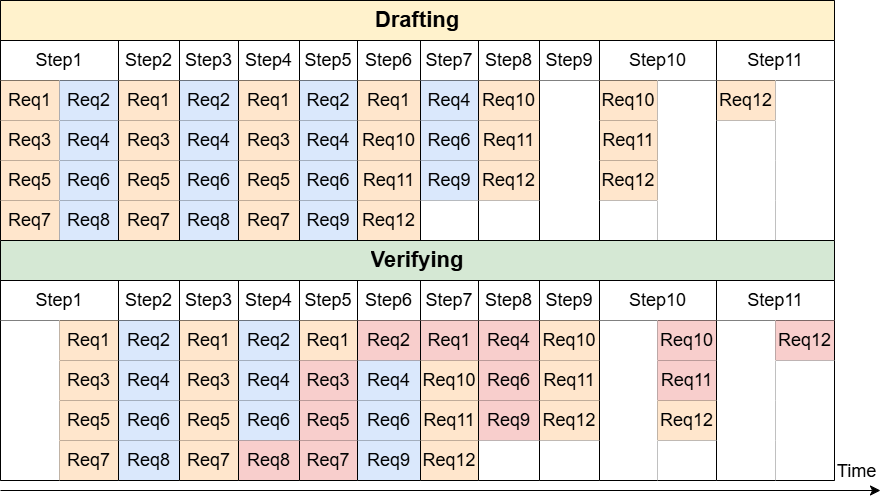
\includegraphics[width=\linewidth]{figures/bp_timeline.png}
    \caption{
        \textbf{Timeline of an example Batch Parallelism lifespan.} Requests with an orange background belong to Batch~$0$, those with a blue background belong to Batch~$1$, and those with a red background have completed execution.
    }
    \label{fig:bp_timeline}
% \end{figure}
  \end{minipage}\hfill % Adds flexible space between them
  % Right Figure
  \begin{minipage}[t]{0.48\textwidth}
% \begin{figure}[!ht]
    \centering
    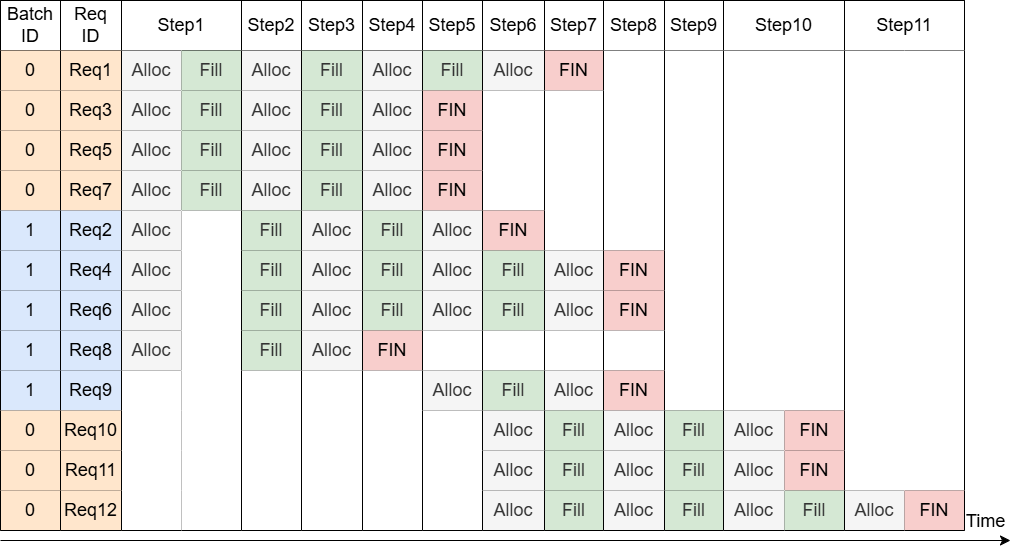
\includegraphics[width=\linewidth]{figures/bp_scheduler.png}
    \caption{
        \textbf{Scheduler perspective of the example Batch Parallelism lifespan.} At each time point, \texttt{Alloc} indicates that the Scheduler allocates KV blocks for a request, \texttt{Fill} indicates that the allocated blocks are populated with updated KV vectors, and \texttt{FIN} indicates that the request has completed.
    }
    \label{fig:bp_scheduler}
  \end{minipage}
\end{figure}

\begin{figure*}[!ht]
    \centering
    \setlength{\tabcolsep}{1pt} 
    \resizebox{0.99\linewidth}{!}{
    \begin{tabular}{ccccc}
        & \hspace{8mm}\textbf{Arena} & \hspace{8mm}\textbf{ShareGPT} & \hspace{8mm}\textbf{Spec-Bench}  & \hspace{8mm}\textbf{Tough}\\
    
        \rotatebox{90}{\parbox{3.5cm}{\centering \hspace{8mm}\textbf{Vicuna~13B-EAGLE}}} &
        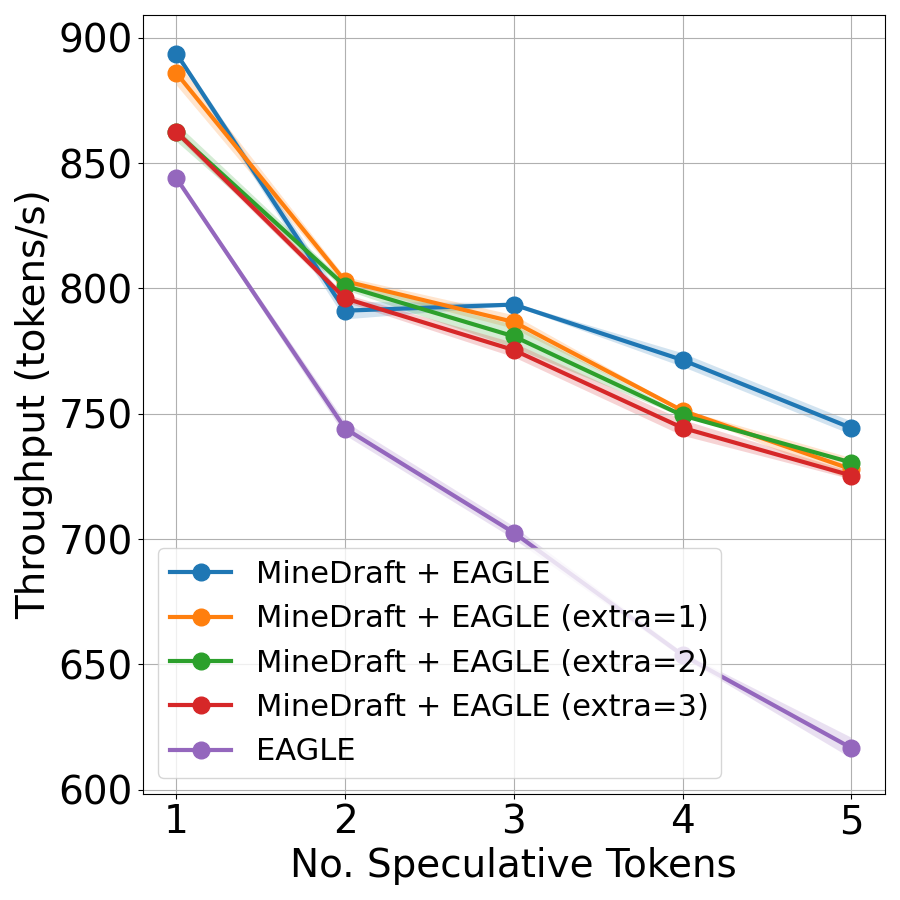
\includegraphics[width=0.23\linewidth]{results/Arena_vicuna-13b-v1_3_EAGLE-Vicuna-13B-v1_3_1000_bs16_100pct_gen_throughput.png} &
        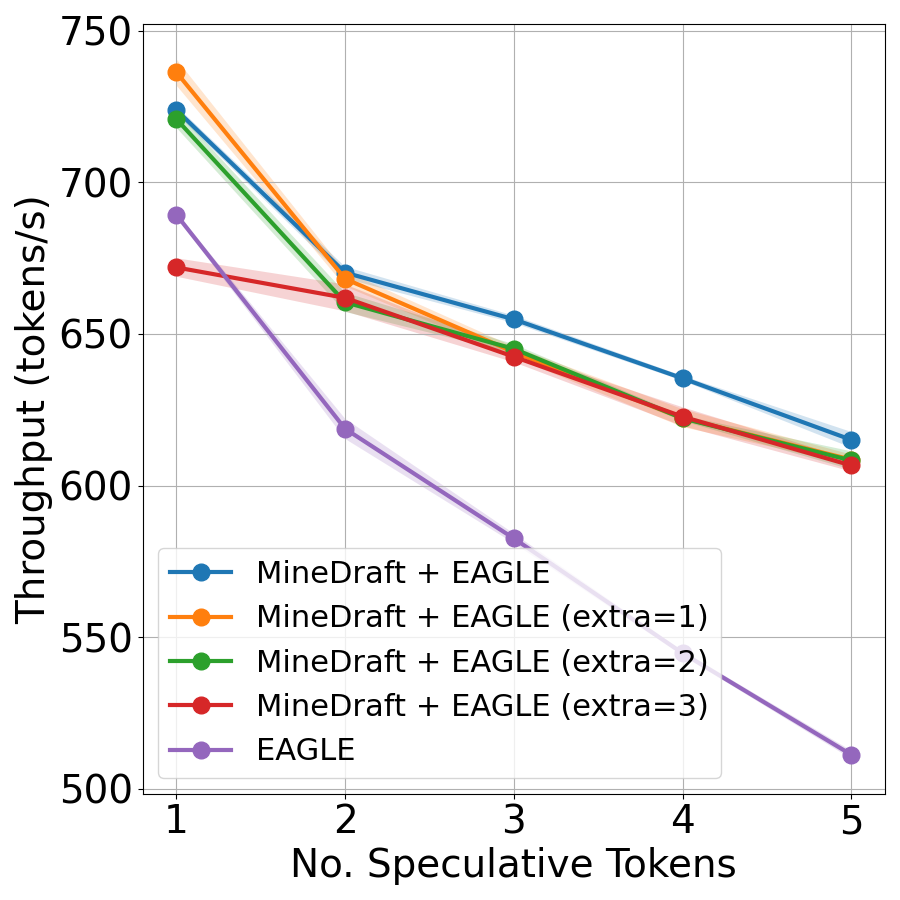
\includegraphics[width=0.23\linewidth]{results/ShareGPT_vicuna-13b-v1_3_EAGLE-Vicuna-13B-v1_3_1000_bs16_100pct_gen_throughput.png} &
        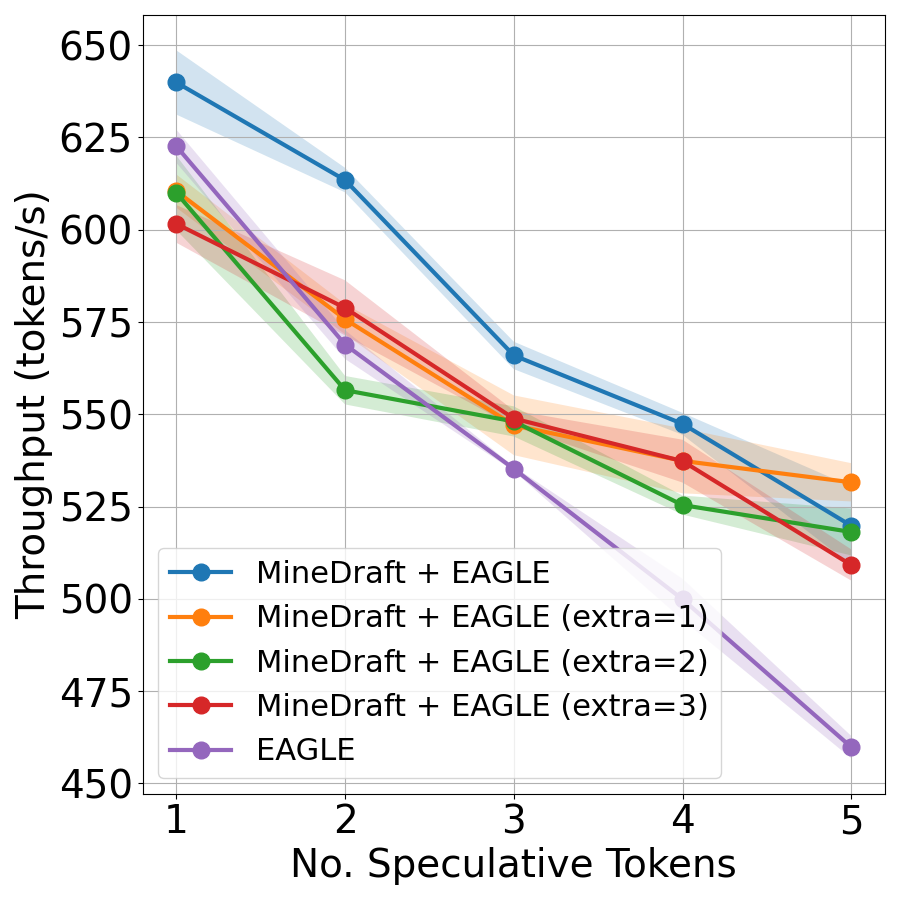
\includegraphics[width=0.23\linewidth]{results/Spec-Bench_vicuna-13b-v1_3_EAGLE-Vicuna-13B-v1_3_162_bs16_100pct_gen_throughput.png} &
        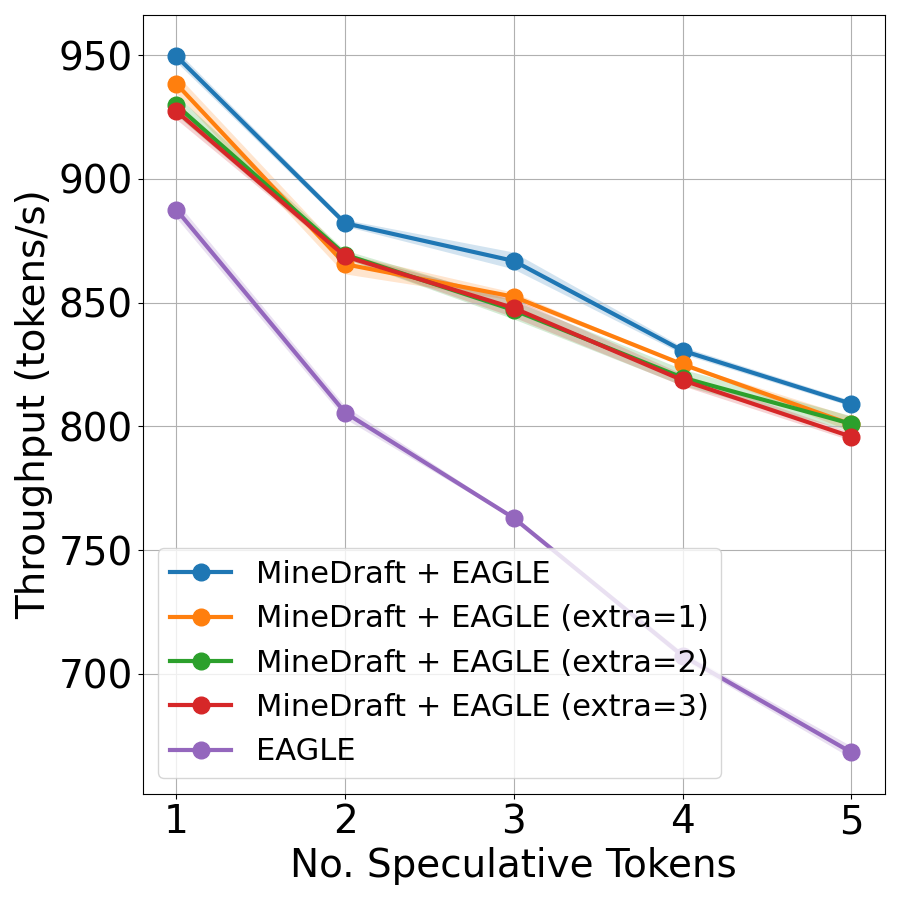
\includegraphics[width=0.23\linewidth]{results/Tough_vicuna-13b-v1_3_EAGLE-Vicuna-13B-v1_3_1000_bs16_100pct_gen_throughput.png} \\
        & \hspace{2mm}(a) \hspace{2mm} $\uparrow$ 5.89\%, $\Delta$ 20.71\% &
        \hspace{2mm}(b) \hspace{2mm} $\uparrow$ 6.82\%, $\Delta$ 20.31\% &
        \hspace{2mm}(c) \hspace{2mm} $\uparrow$ 2.78\%, $\Delta$ 15.60\% &
        \hspace{2mm}(d) \hspace{2mm} $\uparrow$ 6.99\%, $\Delta$ 21.08\% \\

    \end{tabular}}
    \caption{Throughput comparison on model setting 7. $\uparrow$ indicates the average improvement over the best baseline method. $\Delta$ indicates the maximum average gap between \alg{} and EAGLE.
    }
    \label{fig:throughput-eagle-13b}
\end{figure*}


\begin{figure*}[!ht]
    \centering
    \setlength{\tabcolsep}{1pt} 
    \resizebox{0.99\linewidth}{!}{
    \begin{tabular}{ccccc}
        & \hspace{8mm}\textbf{Arena} & \hspace{8mm}\textbf{ShareGPT} & \hspace{8mm}\textbf{Spec-Bench}  & \hspace{8mm}\textbf{Tough}\\
        
        \rotatebox{90}{\parbox{3.5cm}{\centering \hspace{8mm}\textbf{Qwen3~32B-0.6B}}} &
        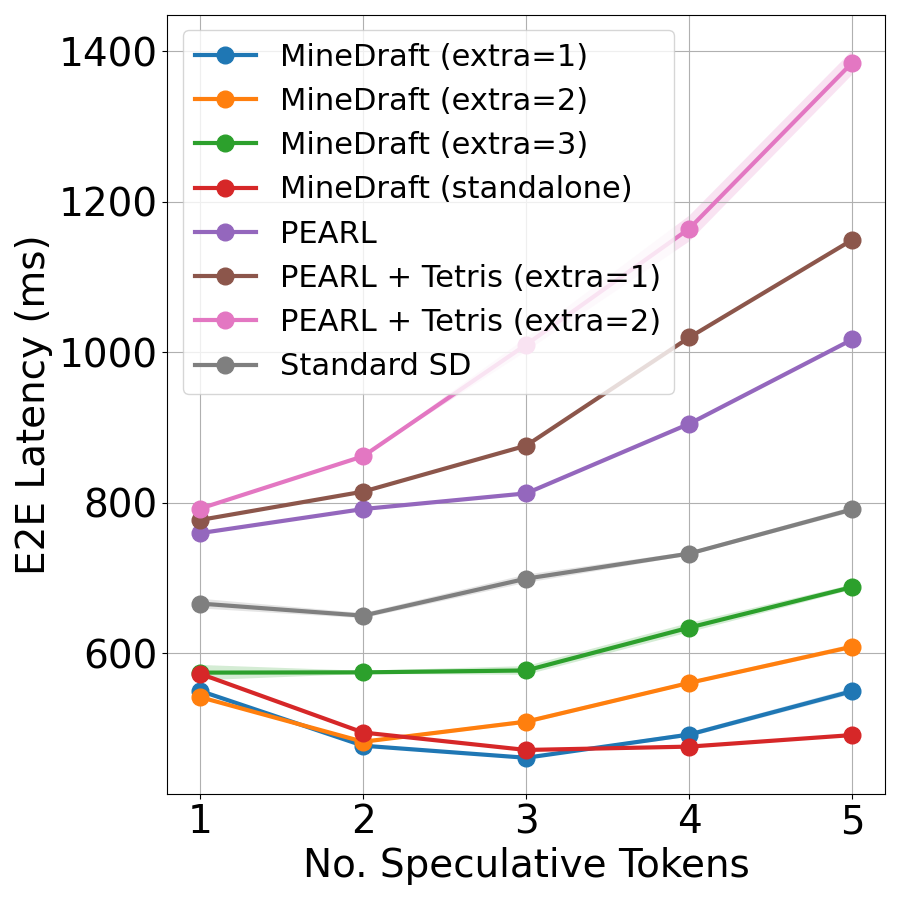
\includegraphics[width=0.23\linewidth]{results/Arena_Qwen3-32B_Qwen3-0_6B_1000_bs16_100pct_latency.png} &
        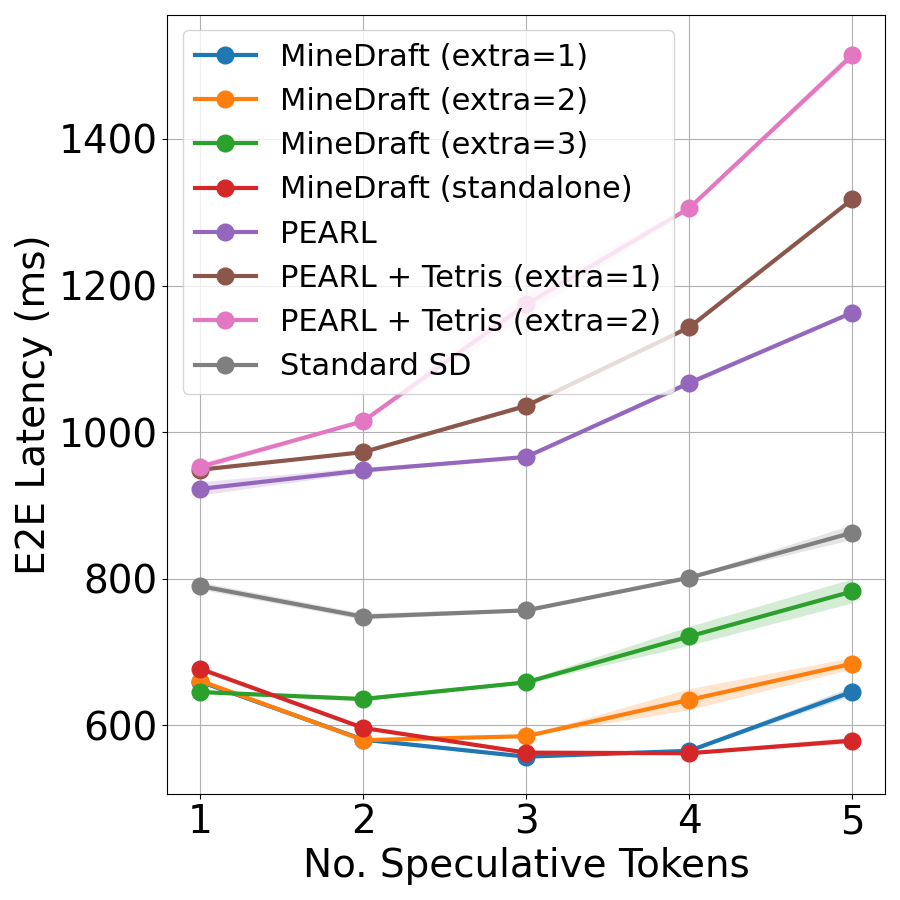
\includegraphics[width=0.23\linewidth]{results/ShareGPT_Qwen3-32B_Qwen3-0_6B_1000_bs16_100pct_latency.png} &
        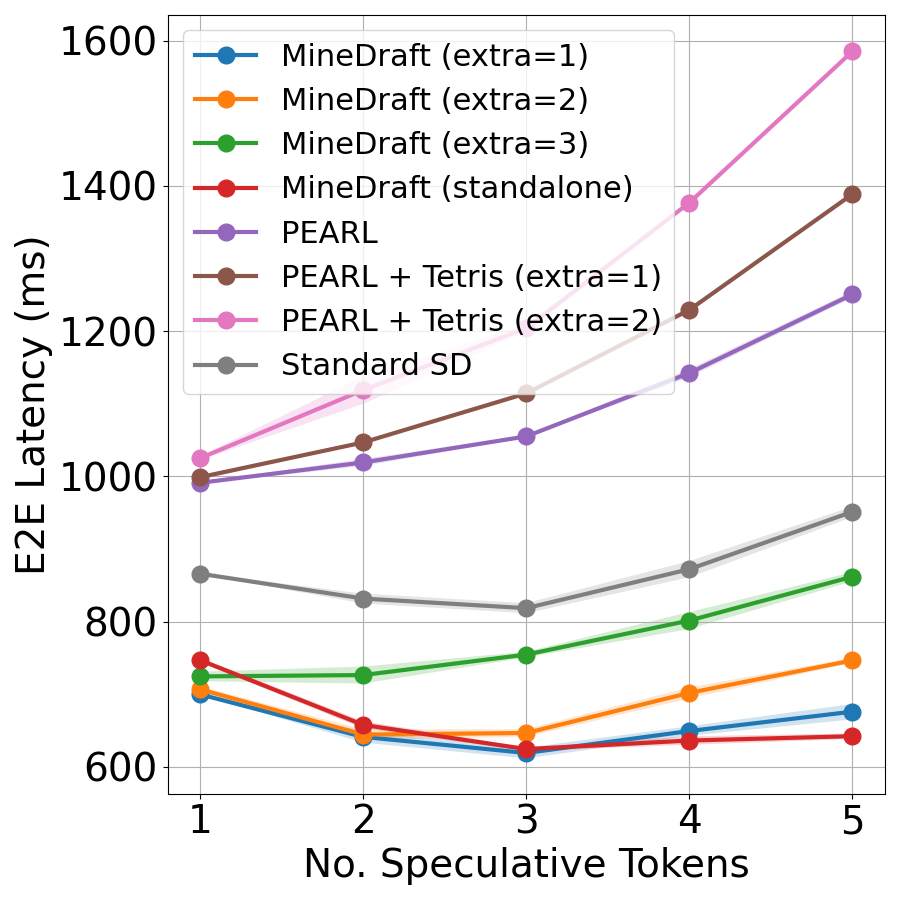
\includegraphics[width=0.23\linewidth]{results/Spec-Bench_Qwen3-32B_Qwen3-0_6B_161_bs16_100pct_latency.png} &
        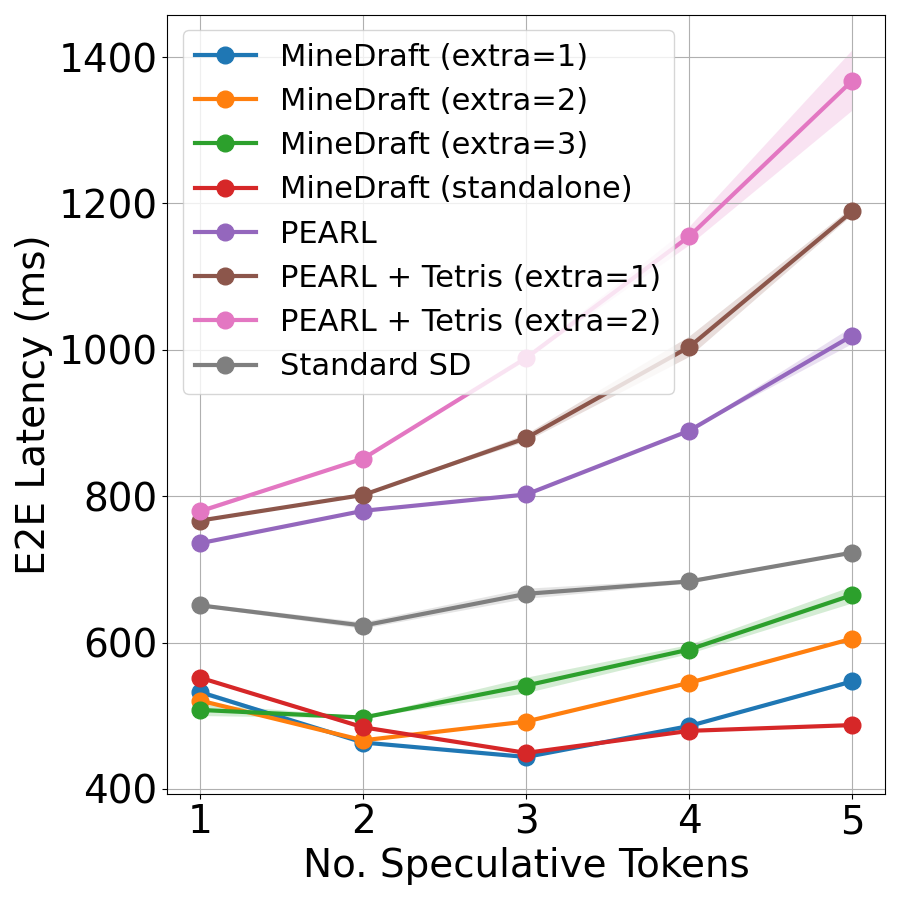
\includegraphics[width=0.23\linewidth]{results/Tough_Qwen3-32B_Qwen3-0_6B_1000_bs16_100pct_latency.png} \\
        & \hspace{2mm}(a) \hspace{2mm} $\uparrow$ 26.58\%, $\Delta$ 37.89\% &
        \hspace{2mm}(b) \hspace{2mm} $\uparrow$ 22.49\%, $\Delta$ 32.87\% &
        \hspace{2mm}(c) \hspace{2mm} $\uparrow$ 24.37\%, $\Delta$ 32.49\% &
        \hspace{2mm}(d) \hspace{2mm} $\uparrow$ 25.63\%, $\Delta$ 33.44\% \\
    
        \rotatebox{90}{\parbox{3.5cm}{\centering \hspace{8mm}\textbf{Qwen3~32B-1.7B}}} &
        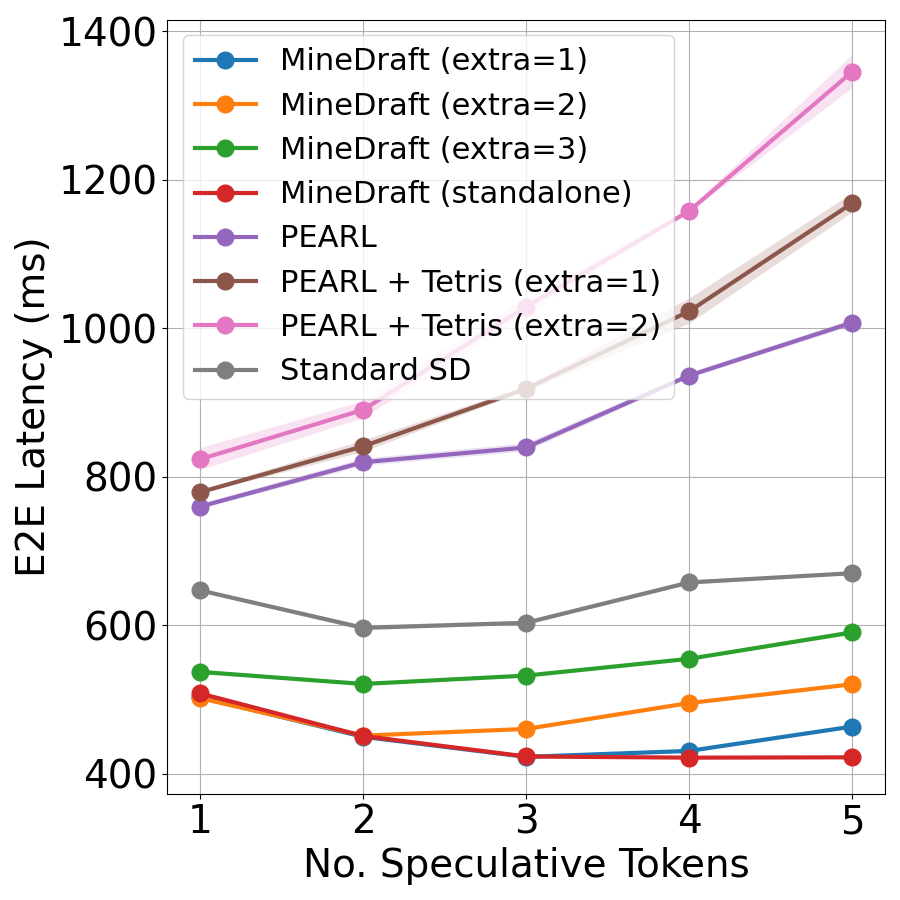
\includegraphics[width=0.23\linewidth]{results/Arena_Qwen3-32B_Qwen3-1_7B_1000_bs16_100pct_latency.png} &
        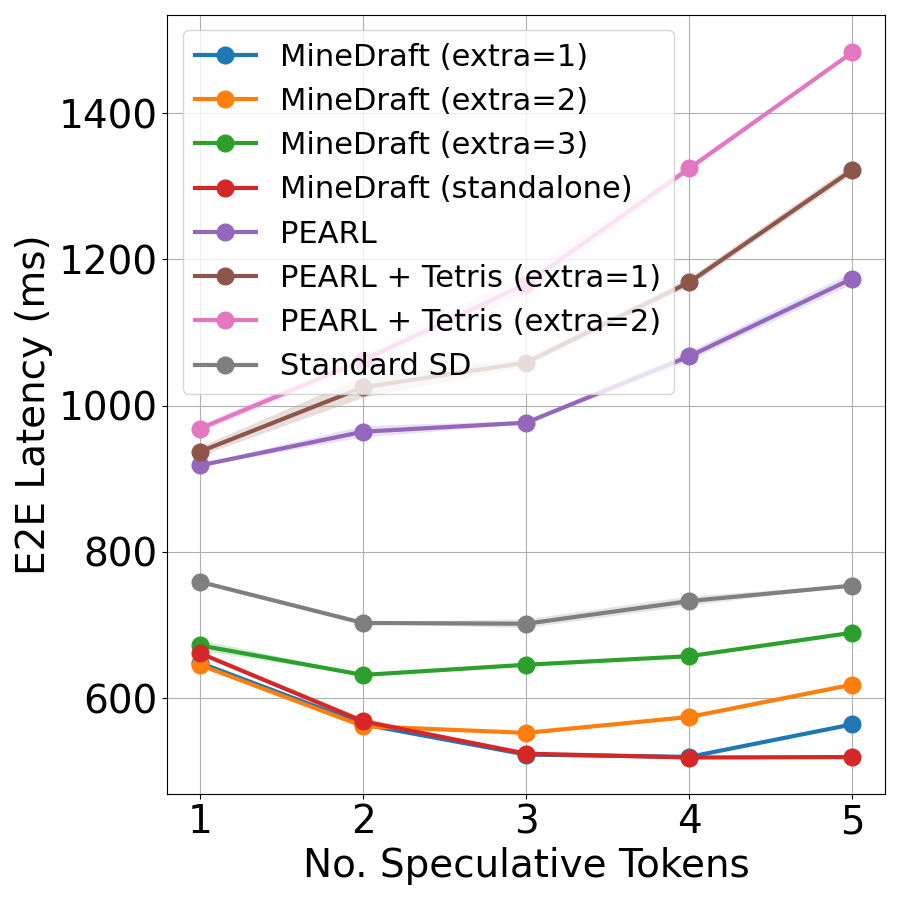
\includegraphics[width=0.23\linewidth]{results/ShareGPT_Qwen3-32B_Qwen3-1_7B_1000_bs16_100pct_latency.png} &
        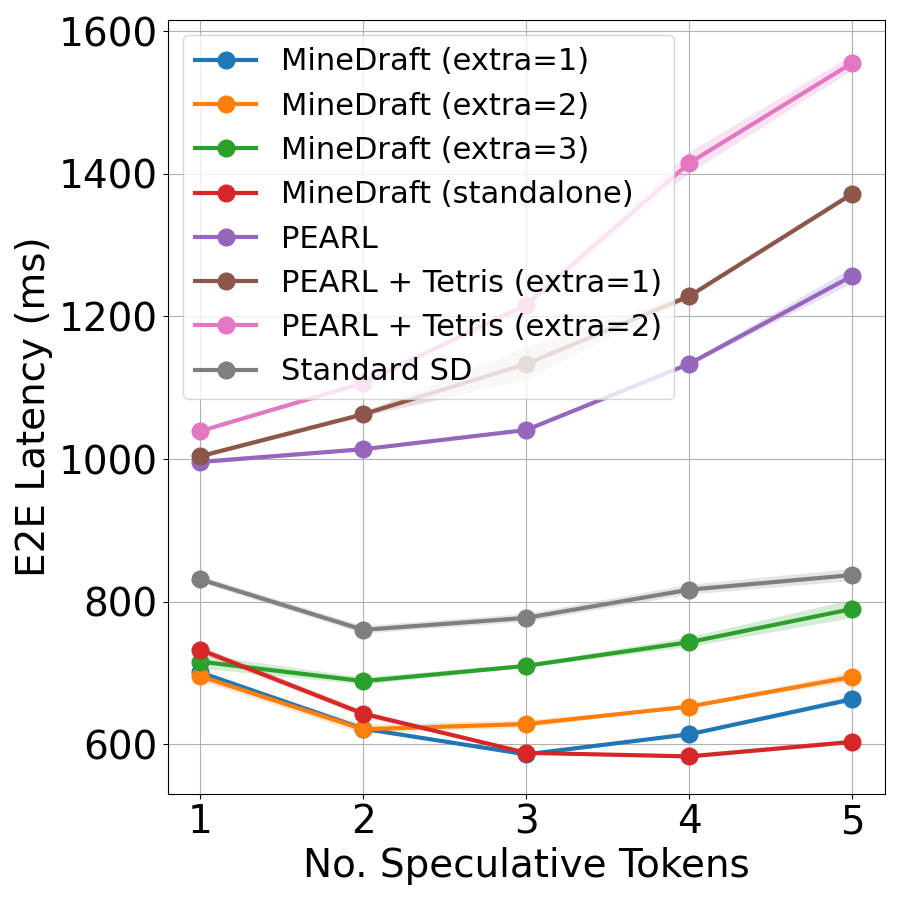
\includegraphics[width=0.23\linewidth]{results/Spec-Bench_Qwen3-32B_Qwen3-1_7B_161_bs16_100pct_latency.png} &
        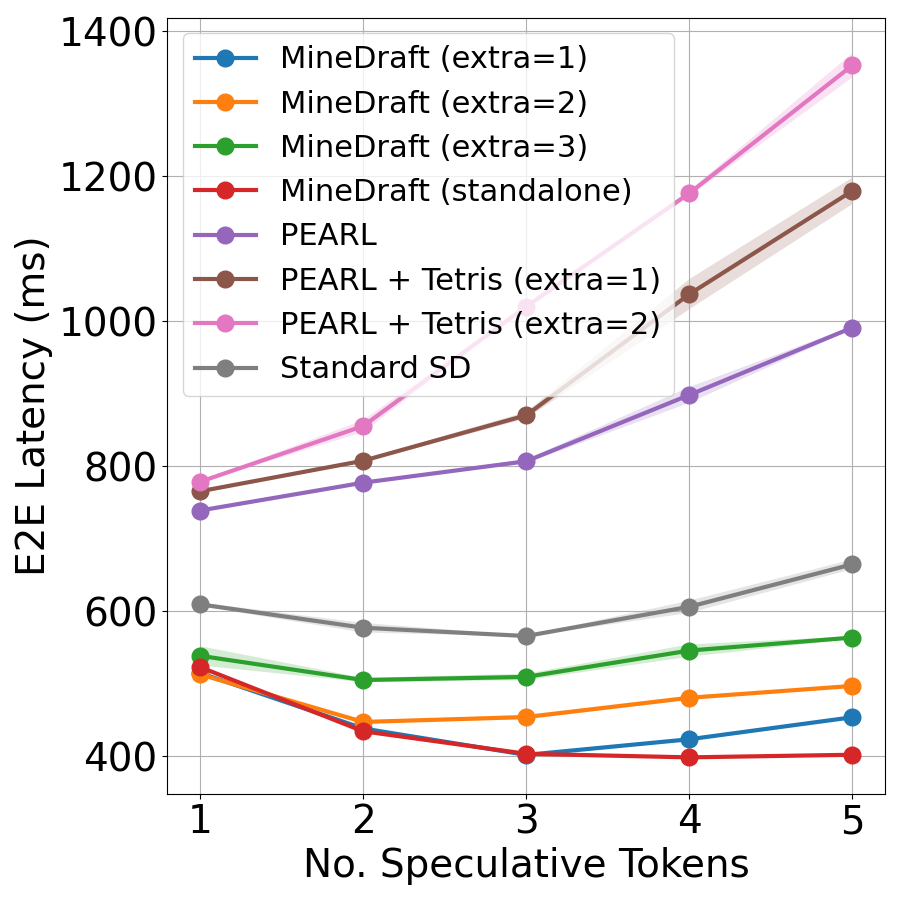
\includegraphics[width=0.23\linewidth]{results/Tough_Qwen3-32B_Qwen3-1_7B_1000_bs16_100pct_latency.png} \\
        & (e) \hspace{2mm} $\uparrow$ 24.59\%, $\Delta$ 36.99\% &
        (f) \hspace{2mm} $\uparrow$ 25.50\%, $\Delta$ 31.09\% &
        (g) \hspace{2mm} $\uparrow$ 18.34\%, $\Delta$ 28.63\% &
        (h) \hspace{2mm} $\uparrow$ 28.97\%, $\Delta$ 39.51\% \\
        
        \rotatebox{90}{\parbox{3.5cm}{\centering \hspace{8mm}\textbf{Qwen3~32B-4B}}} &
        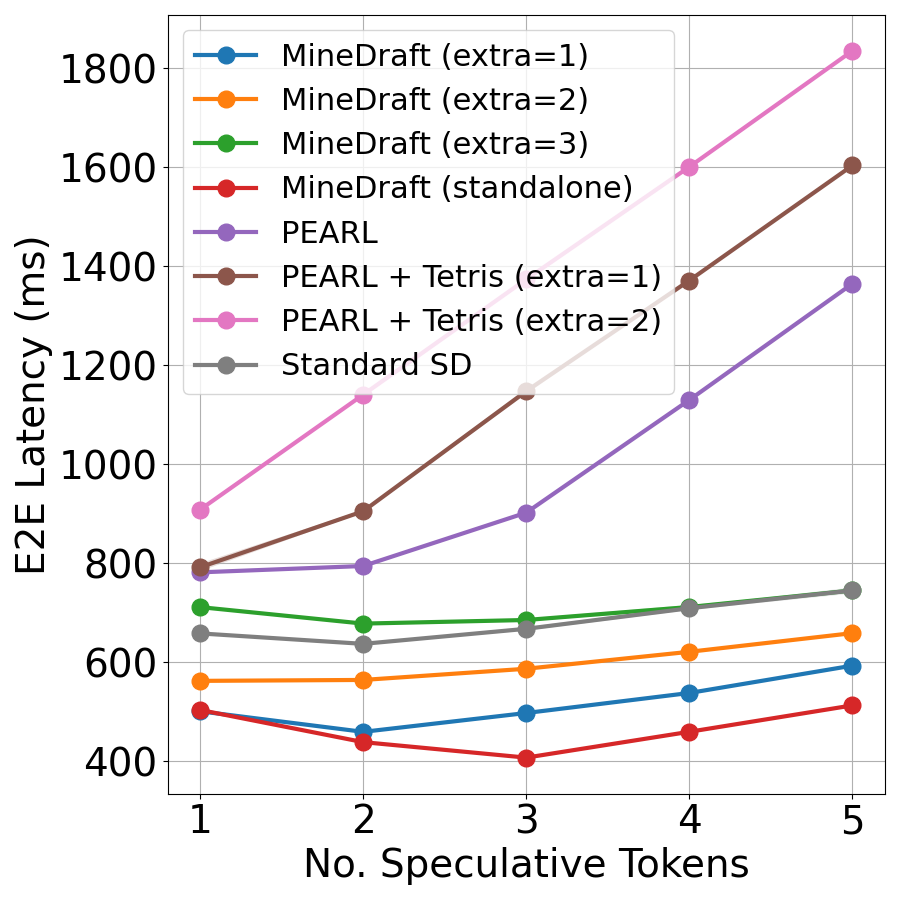
\includegraphics[width=0.23\linewidth]{results/Arena_Qwen3-32B_Qwen3-4B_1000_bs16_100pct_latency.png} &
        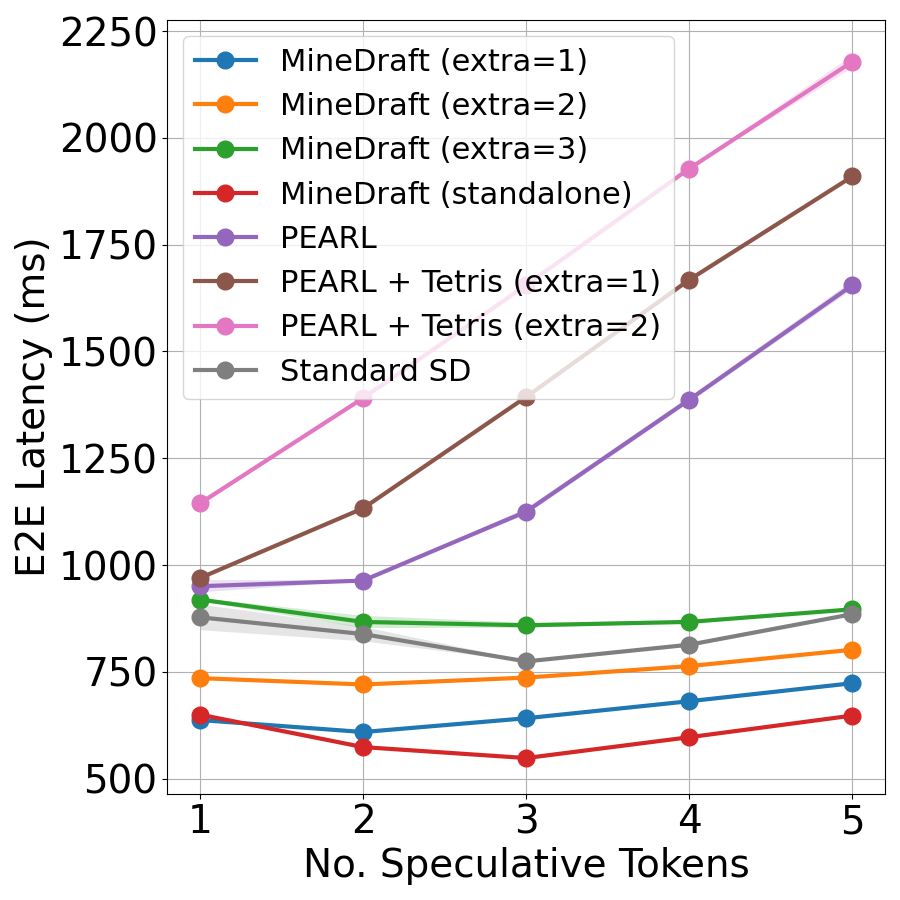
\includegraphics[width=0.23\linewidth]{results/ShareGPT_Qwen3-32B_Qwen3-4B_1000_bs16_100pct_latency.png} &
        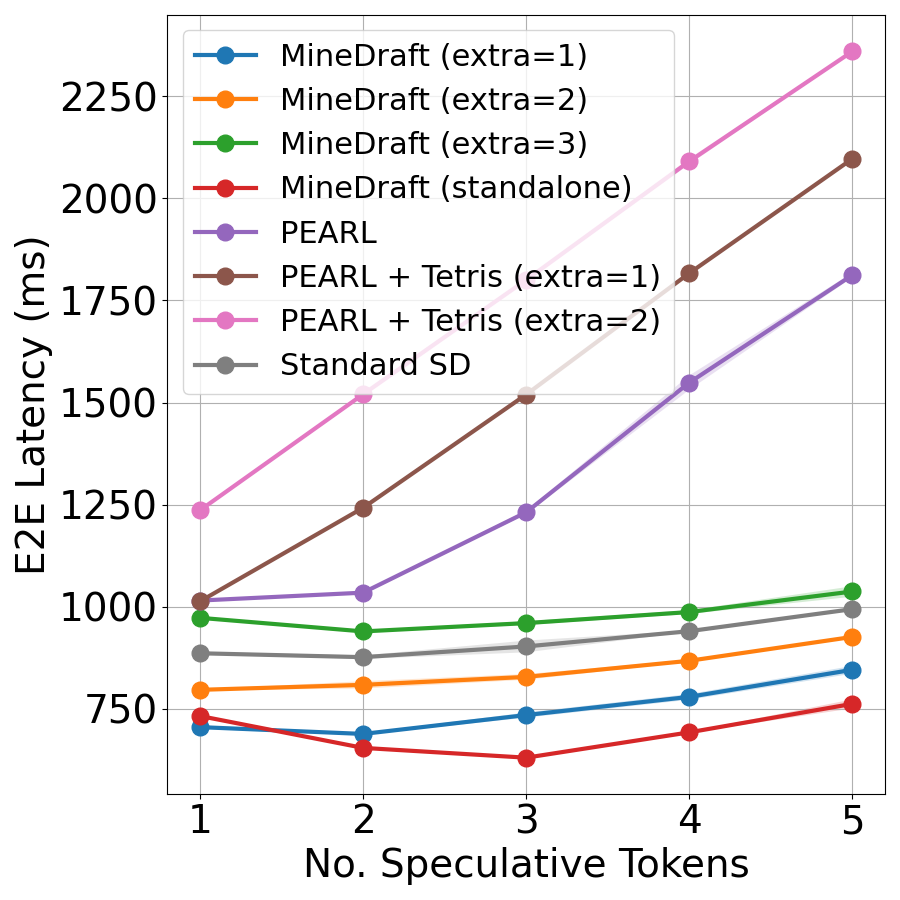
\includegraphics[width=0.23\linewidth]{results/Spec-Bench_Qwen3-32B_Qwen3-4B_161_bs16_100pct_latency.png} &
        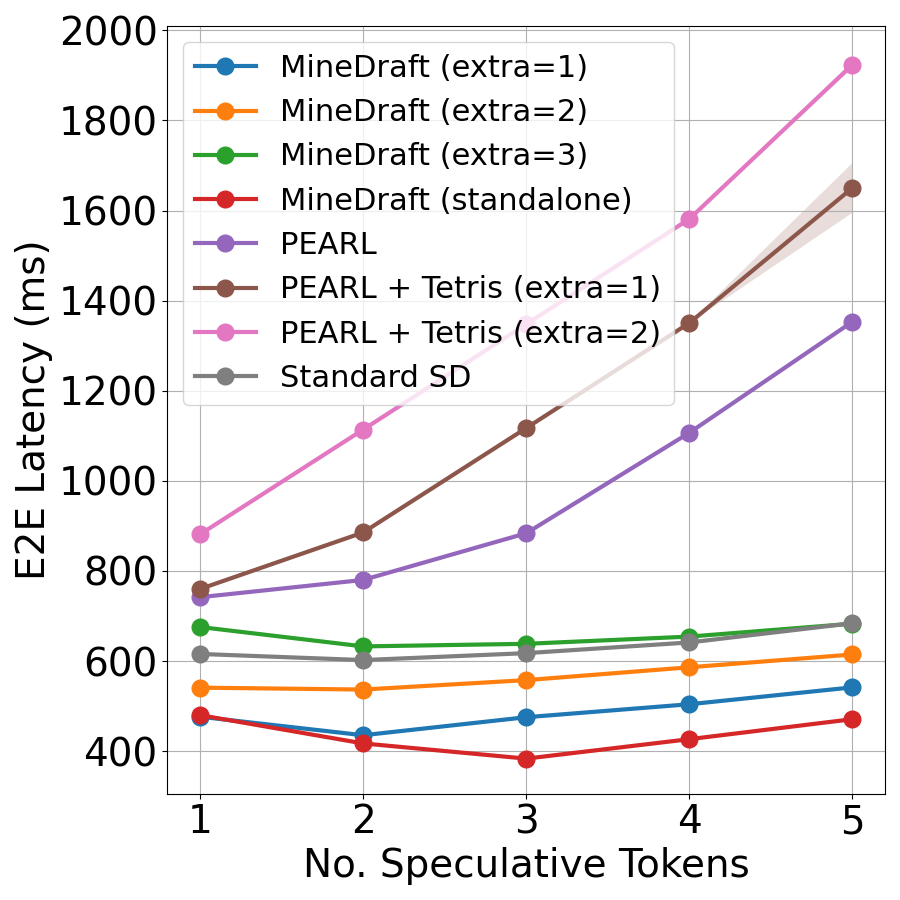
\includegraphics[width=0.23\linewidth]{results/Tough_Qwen3-32B_Qwen3-4B_1000_bs16_100pct_latency.png} \\
        & \hspace{2mm}(i) \hspace{2mm} $\uparrow$ 31.13\%, $\Delta$ 38.94\% &
        \hspace{2mm}(j) \hspace{2mm} $\uparrow$ 29.22\%, $\Delta$ 31.57\% &
        \hspace{2mm}(k) \hspace{2mm} $\uparrow$ 25.36\%, $\Delta$ 30.18\% &
        \hspace{2mm}(l) \hspace{2mm} $\uparrow$ 30.73\%, $\Delta$ 37.92\% \\
    \end{tabular}}
    \caption{End-to-End Latency (ms) comparison against baseline methods across model settings 1--3. $\uparrow$ indicates the average improvement over the best baseline method. $\Delta$ indicates the maximum average gap between \alg{} and standard SD.
    }
    \label{fig:e2elatencty-baseline}
\end{figure*}


\begin{figure*}[!ht]
    \centering
    \setlength{\tabcolsep}{1pt} 
    \resizebox{0.99\linewidth}{!}{
    \begin{tabular}{ccccc}
        & \hspace{8mm}\textbf{Arena} & \hspace{8mm}\textbf{ShareGPT} & \hspace{8mm}\textbf{Spec-Bench}  & \hspace{8mm}\textbf{Tough}\\
        \rotatebox{90}{\parbox{3.5cm}{\centering \hspace{8mm}\textbf{Qwen3~32B-8B}}} & 
        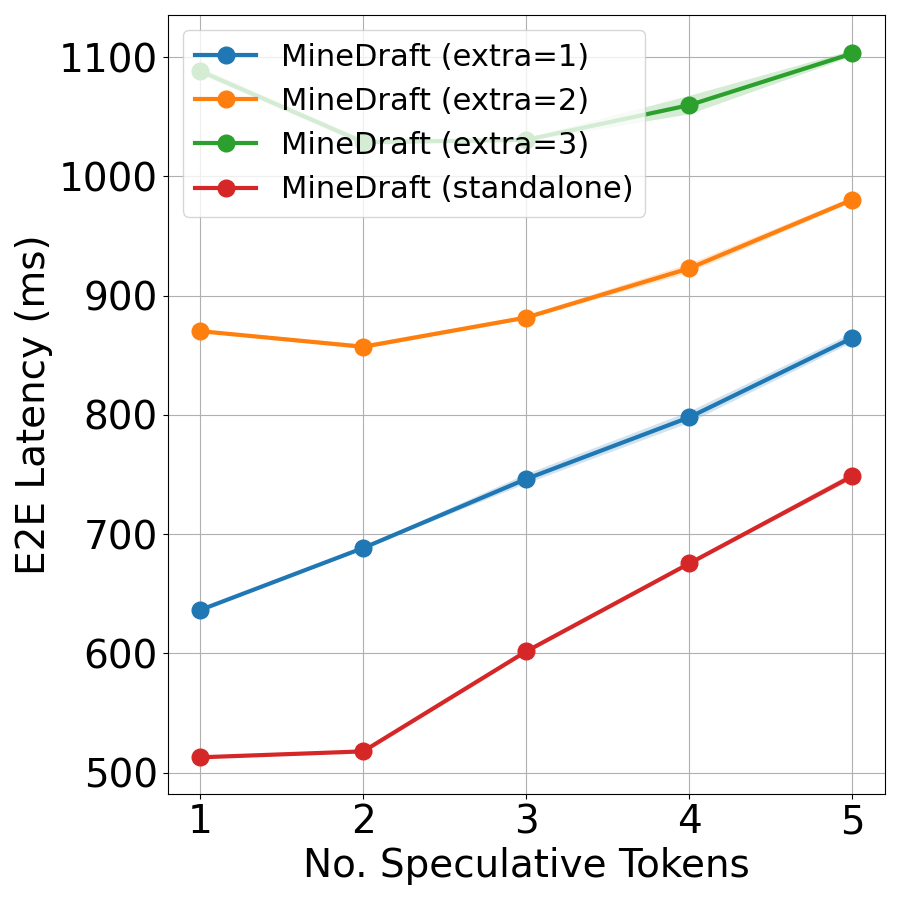
\includegraphics[width=0.23\linewidth]{results/Arena_Qwen3-32B_Qwen3-8B_1000_bs16_100pct_latency.png} &
        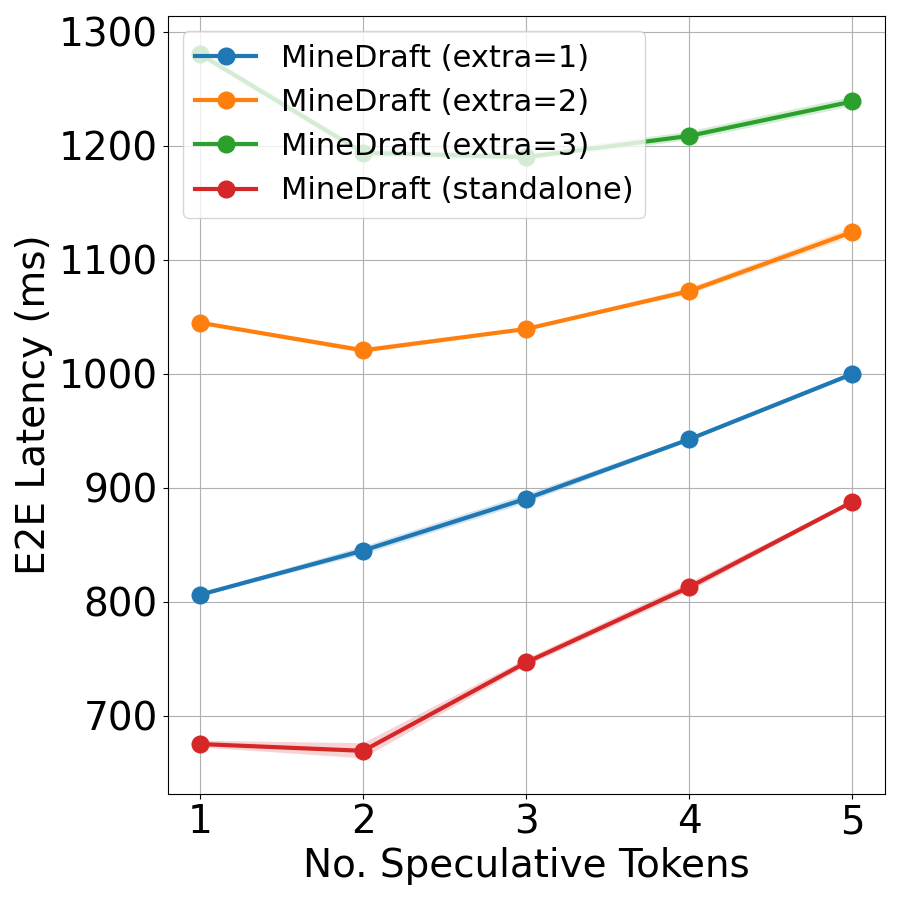
\includegraphics[width=0.23\linewidth]{results/ShareGPT_Qwen3-32B_Qwen3-8B_1000_bs16_100pct_latency.png} &
        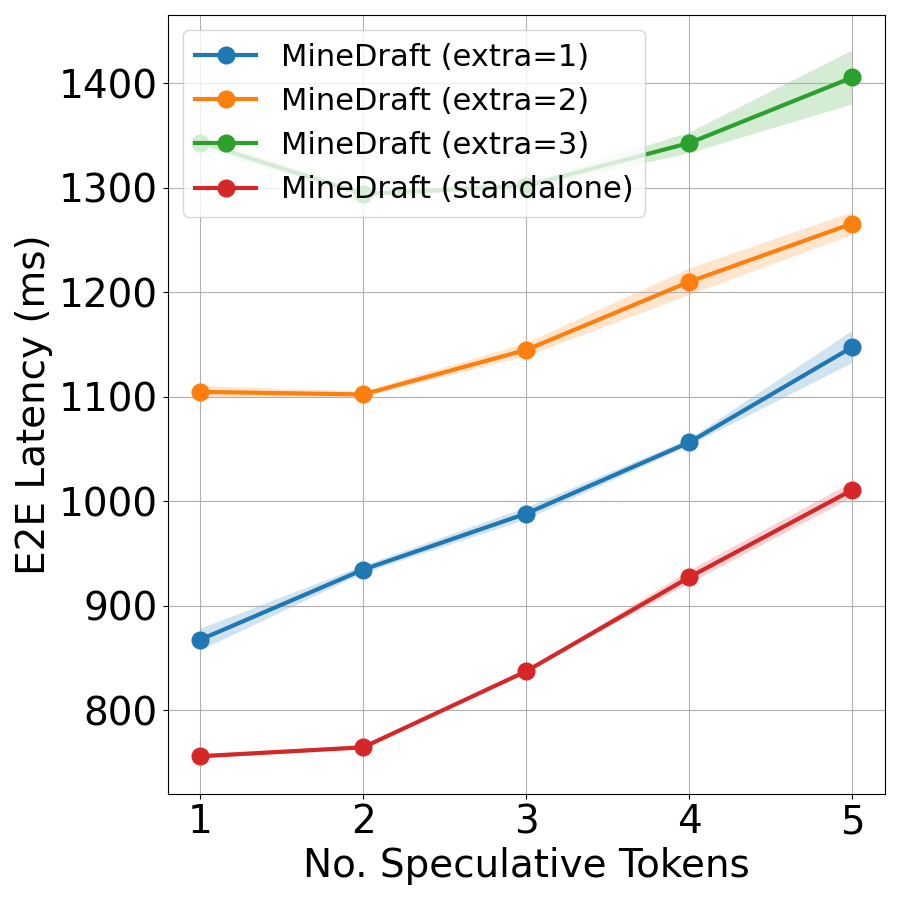
\includegraphics[width=0.23\linewidth]{results/Spec-Bench_Qwen3-32B_Qwen3-8B_161_bs16_100pct_latency.png} &
        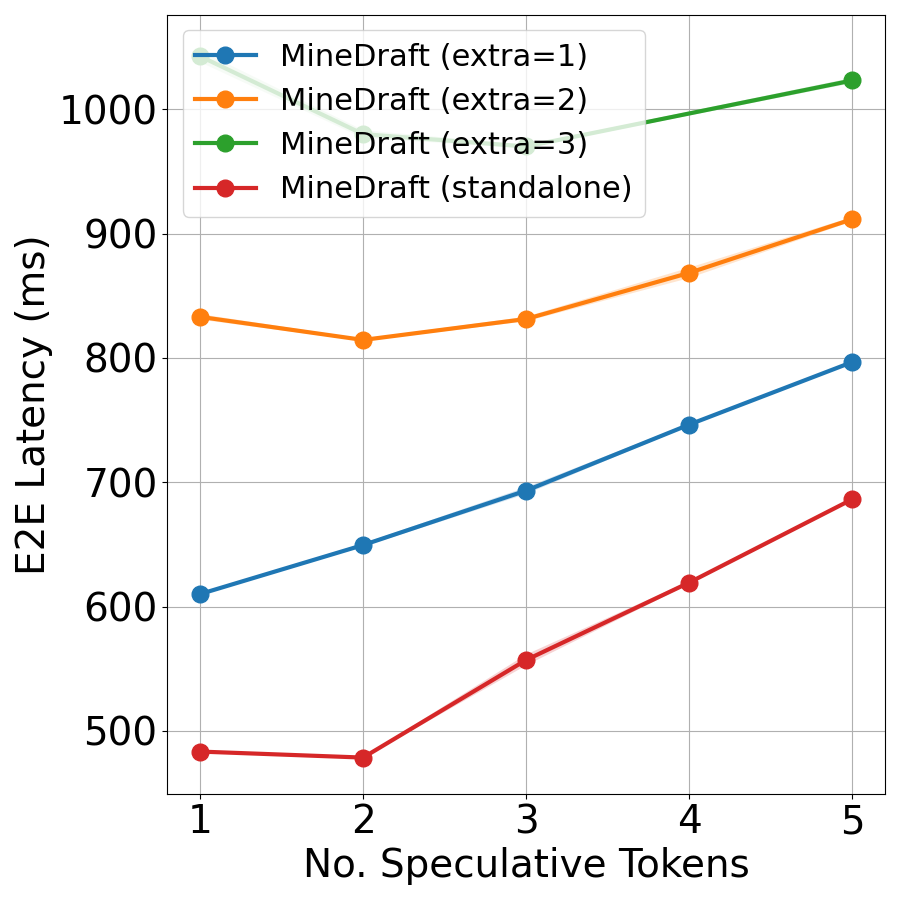
\includegraphics[width=0.23\linewidth]{results/Tough_Qwen3-32B_Qwen3-8B_1000_bs16_100pct_latency.png} \\
    \end{tabular}}
    \caption{End-to-End Latency (ms) results on model setting 4.
    }
    \label{fig:e2elatencty-qwen8b}
\end{figure*}


\begin{figure*}[!ht]
    \centering
    \setlength{\tabcolsep}{1pt} 
    \resizebox{0.99\linewidth}{!}{
    \begin{tabular}{ccccc}
        & \hspace{8mm}\textbf{Arena} & \hspace{8mm}\textbf{ShareGPT} & \hspace{8mm}\textbf{Spec-Bench}  & \hspace{8mm}\textbf{Tough}\\
        \rotatebox{90}{\parbox{3.5cm}{\centering \hspace{8mm}\textbf{Llama-3~70B-8B}}} & 
        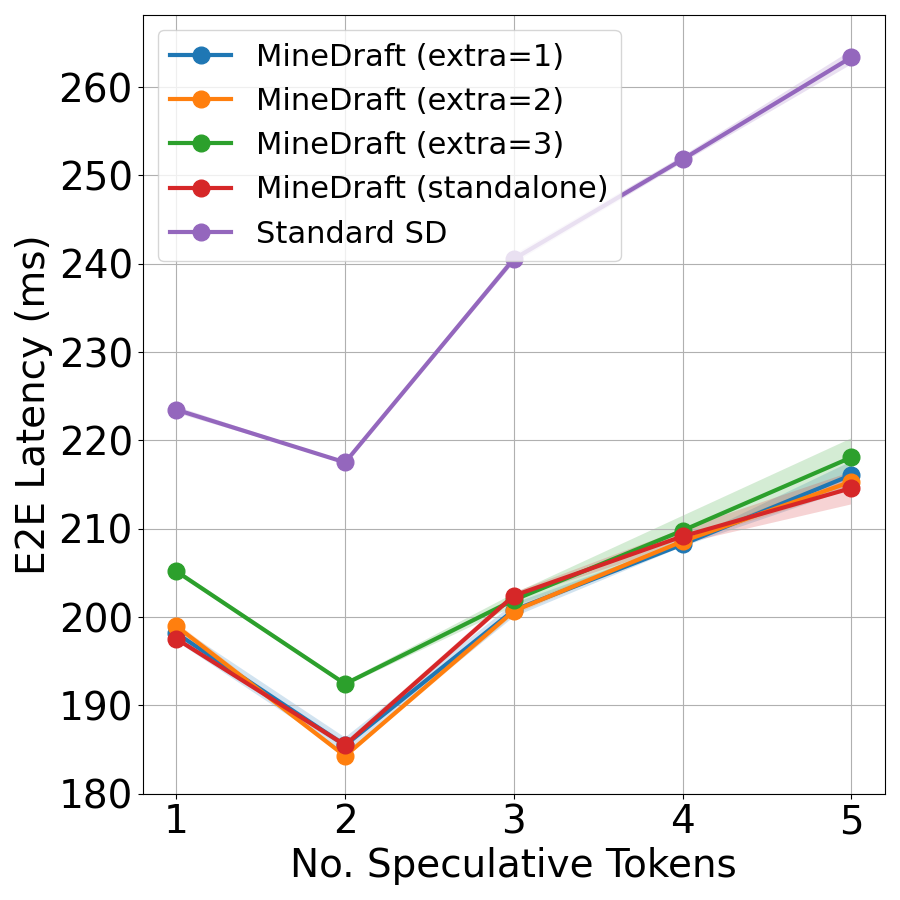
\includegraphics[width=0.23\linewidth]{results/Arena_Meta-Llama-3_3-70B-Instruct-AWQ-INT4_Llama-3_1-8B-Instruct_1000_bs64_100pct_latency.png} &
        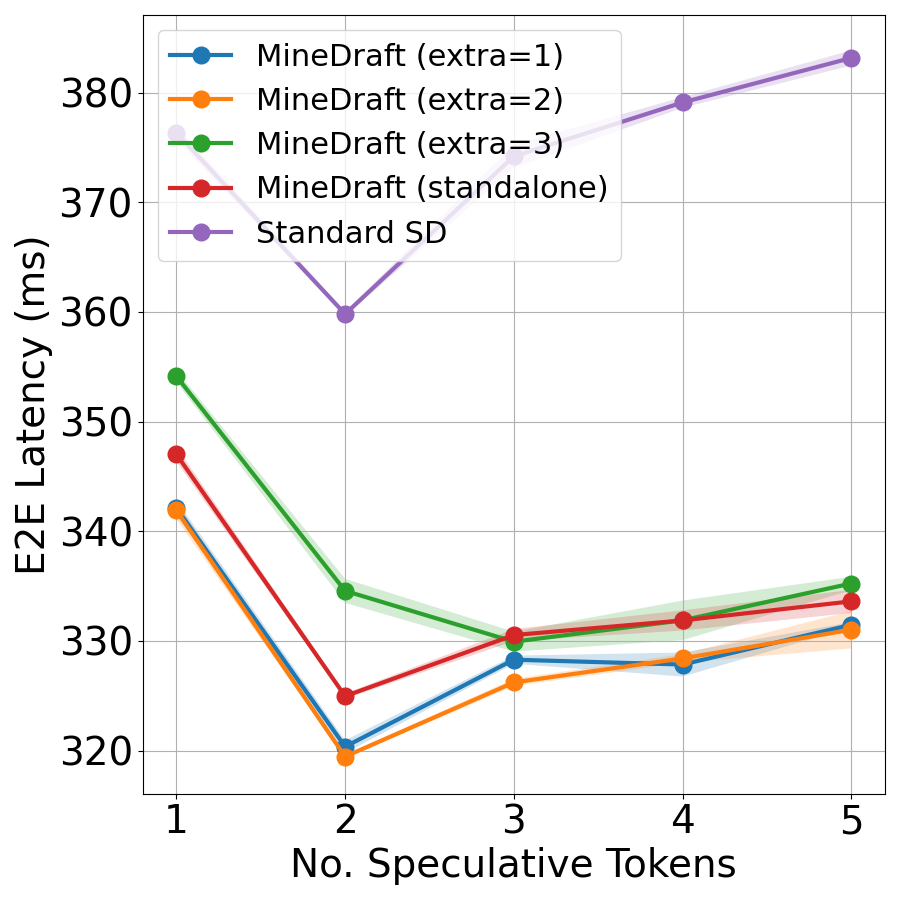
\includegraphics[width=0.23\linewidth]{results/ShareGPT_Meta-Llama-3_3-70B-Instruct-AWQ-INT4_Llama-3_1-8B-Instruct_1000_bs64_100pct_latency.png} &
        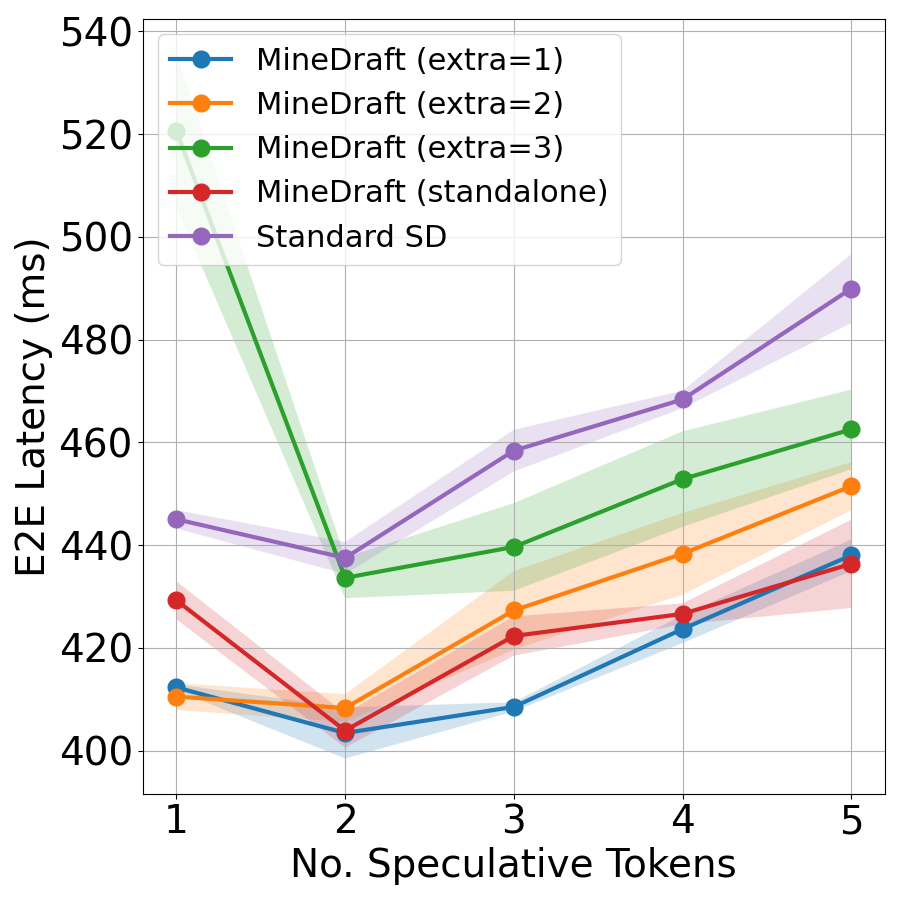
\includegraphics[width=0.23\linewidth]{results/Spec-Bench_Meta-Llama-3_3-70B-Instruct-AWQ-INT4_Llama-3_1-8B-Instruct_160_bs64_100pct_latency.png} &
        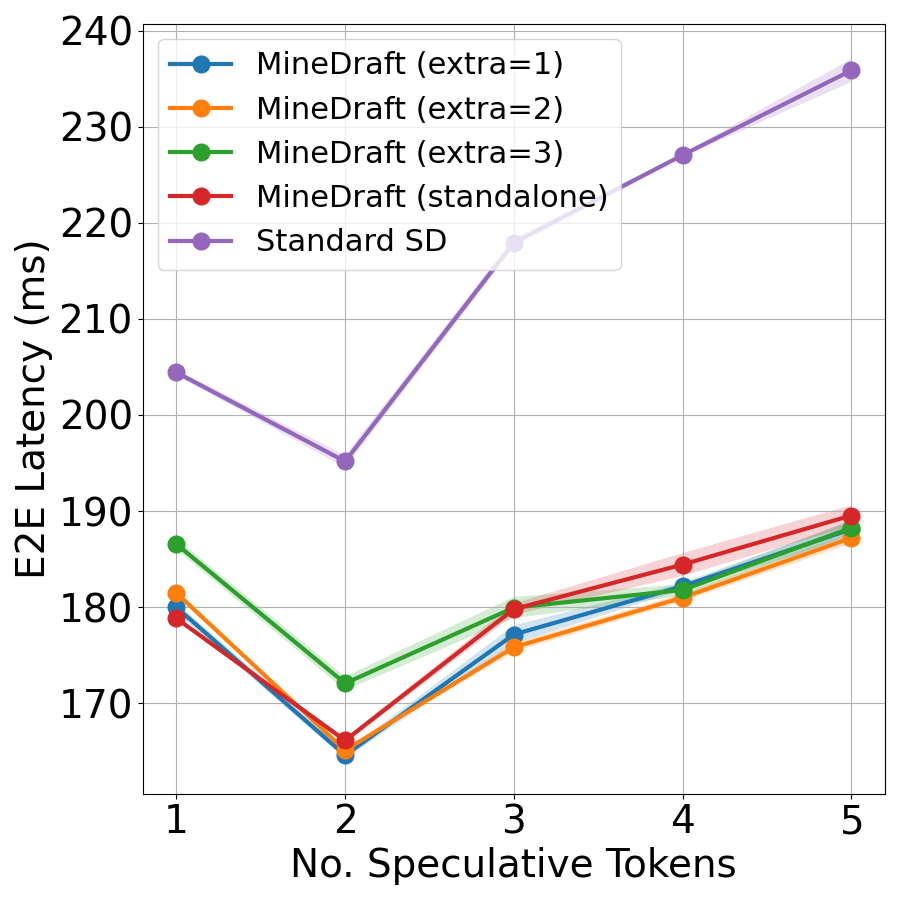
\includegraphics[width=0.23\linewidth]{results/Tough_Meta-Llama-3_3-70B-Instruct-AWQ-INT4_Llama-3_1-8B-Instruct_1000_bs64_100pct_latency.png} \\
        & (a) \hspace{2mm} $\uparrow$ 15.28\%, $\Delta$ 18.52\% &
        (b) \hspace{2mm} $\uparrow$ 11.22\%, $\Delta$ 13.61\% &
        (c) \hspace{2mm} $\uparrow$ 7.79\%, $\Delta$ 10.93\% &
        (d) \hspace{2mm} $\uparrow$ 15.67\%, $\Delta$ 20.63\% \\

        \rotatebox{90}{\parbox{3.5cm}{\centering \hspace{8mm}\textbf{Vicuna~33B-EAGLE}}} &
        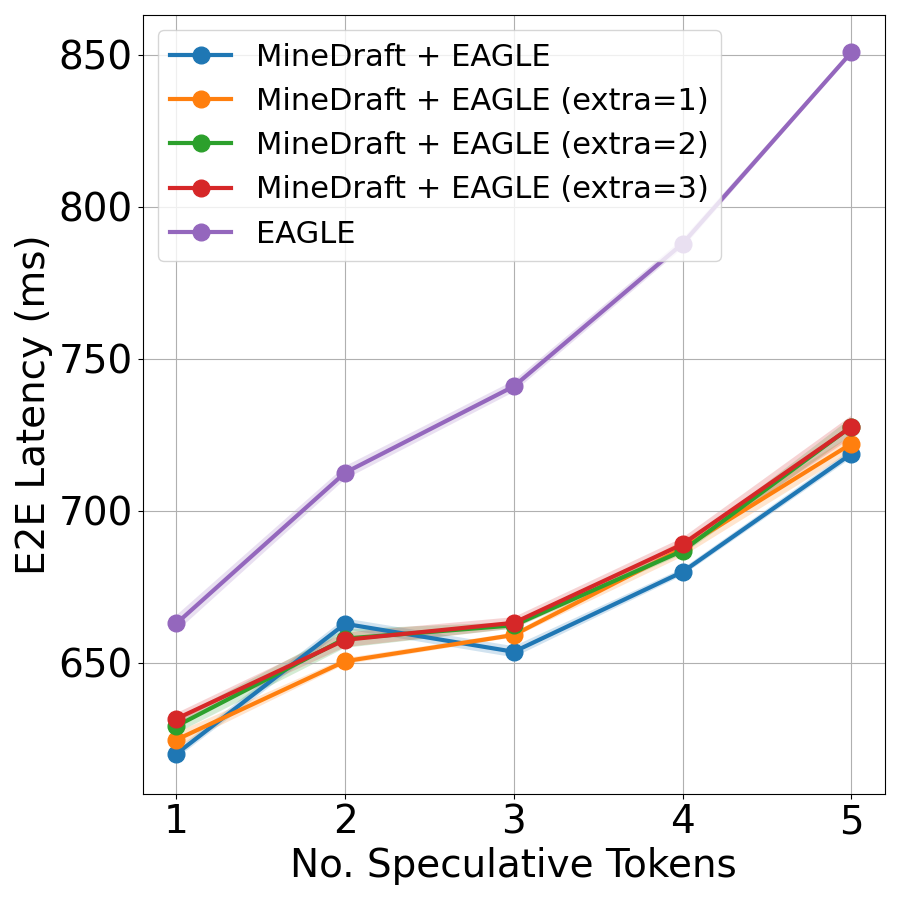
\includegraphics[width=0.23\linewidth]{results/Arena_vicuna-33b-v1_3_EAGLE-Vicuna-33B-v1_3_1000_bs16_100pct_latency.png} &
        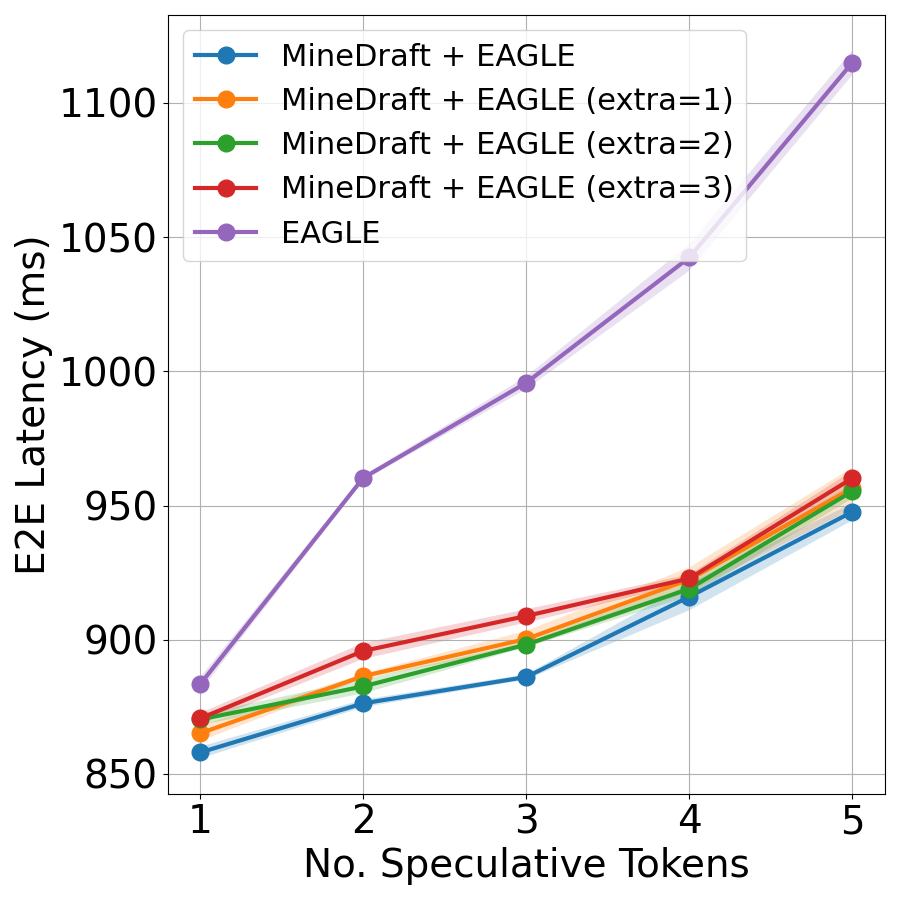
\includegraphics[width=0.23\linewidth]{results/ShareGPT_vicuna-33b-v1_3_EAGLE-Vicuna-33B-v1_3_1000_bs16_100pct_latency.png} &
        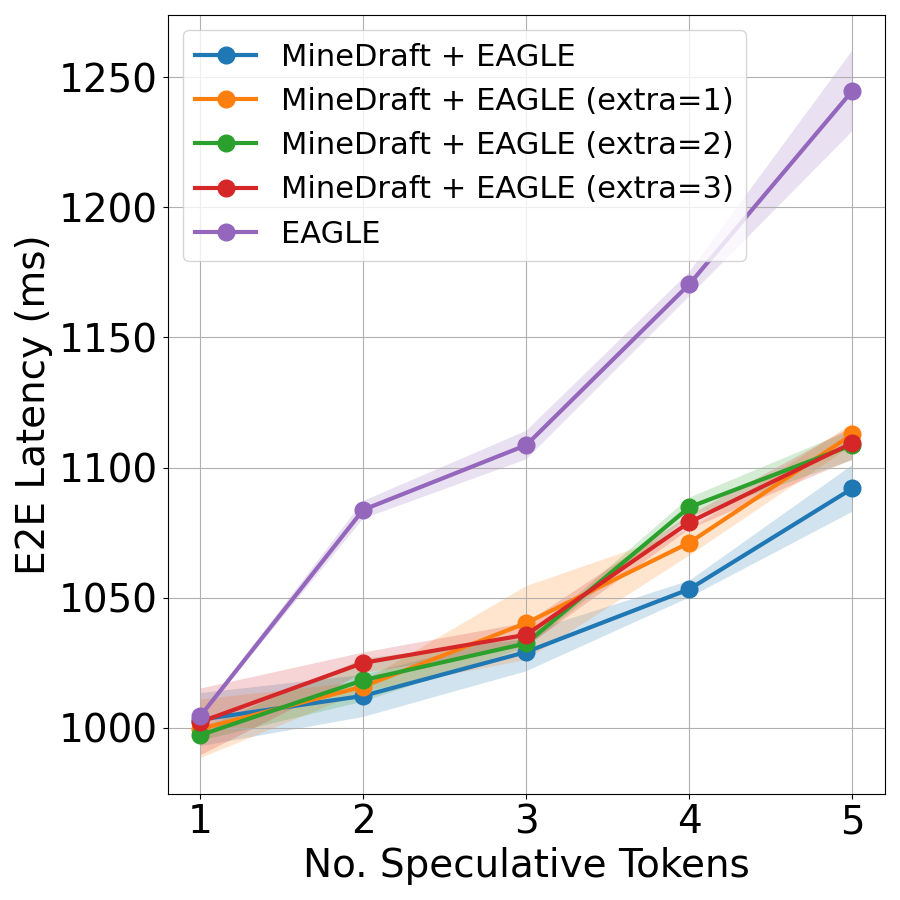
\includegraphics[width=0.23\linewidth]{results/Spec-Bench_vicuna-33b-v1_3_EAGLE-Vicuna-33B-v1_3_162_bs16_100pct_latency.png} &
        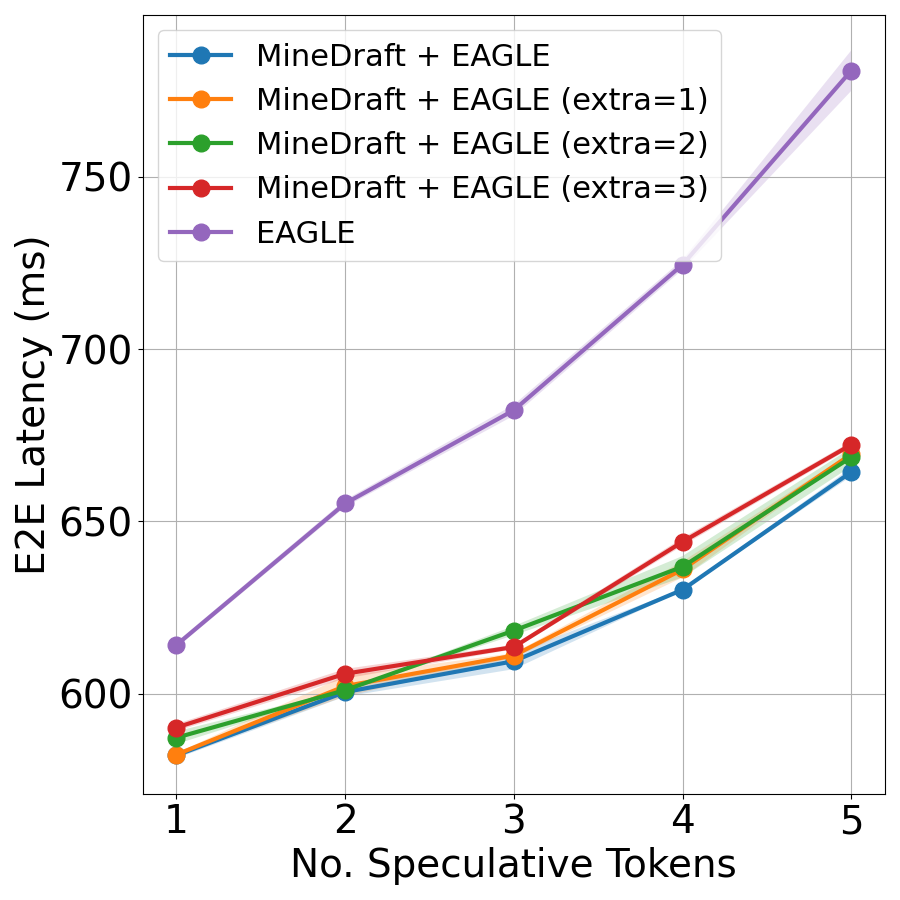
\includegraphics[width=0.23\linewidth]{results/Tough_vicuna-33b-v1_3_EAGLE-Vicuna-33B-v1_3_1000_bs16_100pct_latency.png} \\
        & \hspace{2mm}(e) \hspace{2mm} $\uparrow$ 6.47\%, $\Delta$ 15.52\% &
        \hspace{2mm}(f) \hspace{2mm} $\uparrow$ 2.88\%, $\Delta$ 15.01\% &
        \hspace{2mm}(g) \hspace{2mm} $\uparrow$ 0.72\%, $\Delta$ 12.27\% &
        \hspace{2mm}(h) \hspace{2mm} $\uparrow$ 5.22\%, $\Delta$ 14.93\% \\

        \rotatebox{90}{\parbox{3.5cm}{\centering \hspace{8mm}\textbf{Vicuna~13B-EAGLE}}} &
        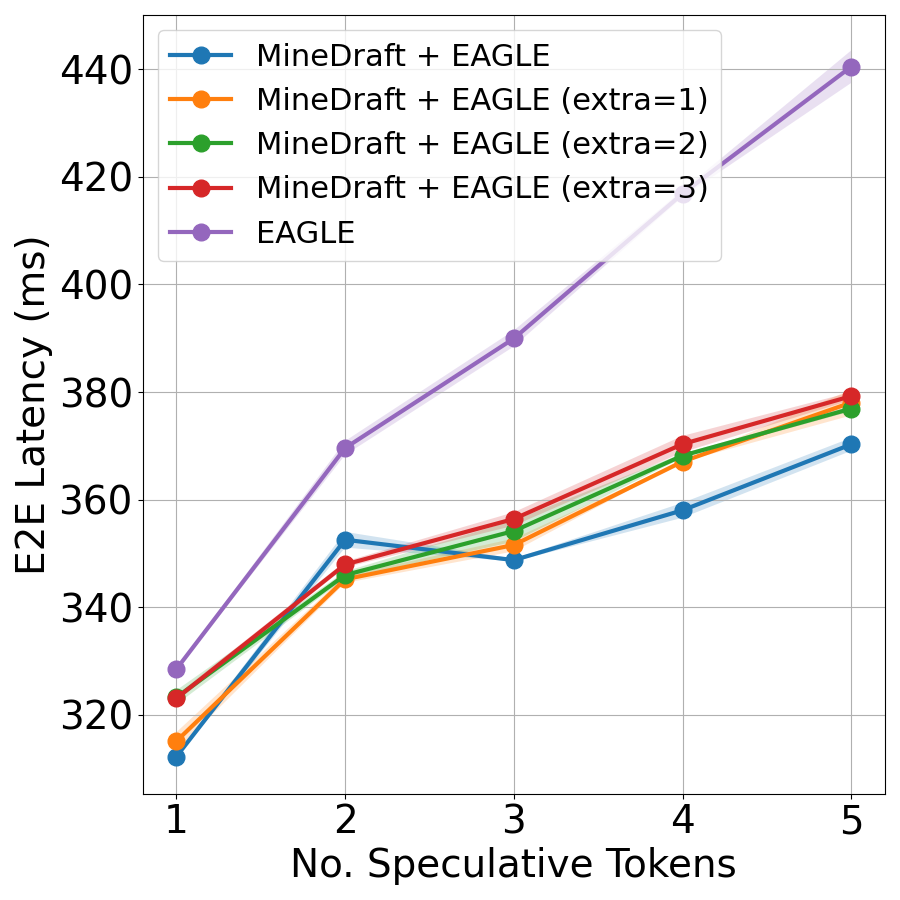
\includegraphics[width=0.23\linewidth]{results/Arena_vicuna-13b-v1_3_EAGLE-Vicuna-13B-v1_3_1000_bs16_100pct_latency.png} &
        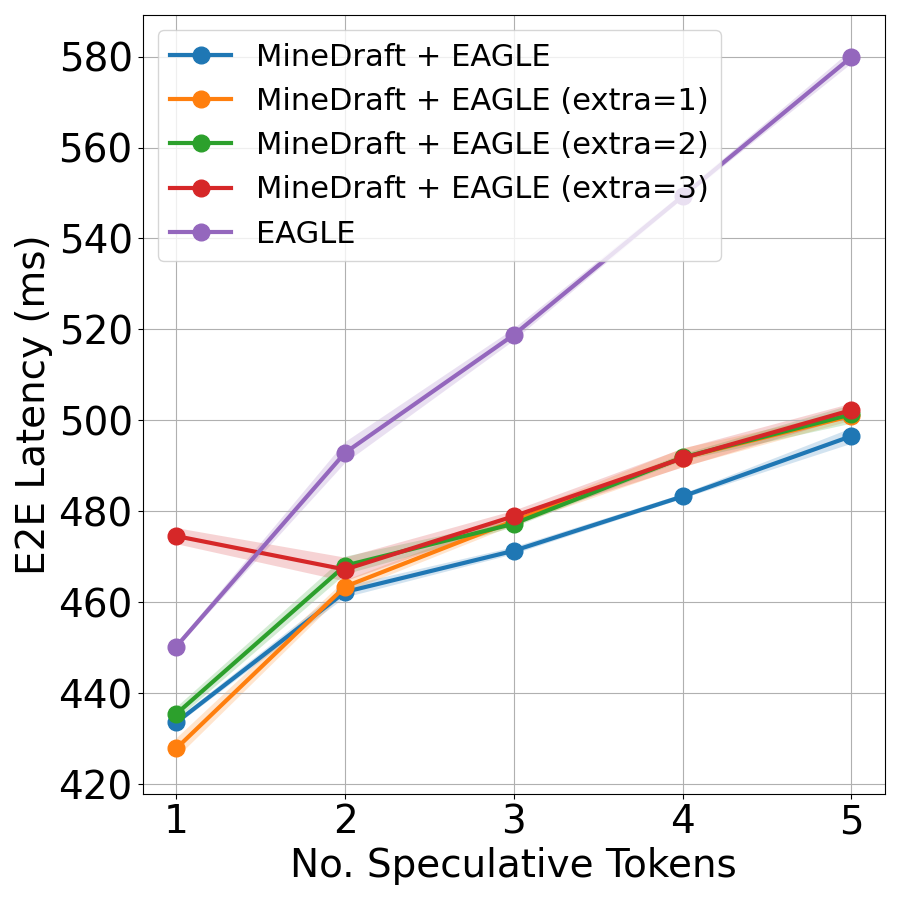
\includegraphics[width=0.23\linewidth]{results/ShareGPT_vicuna-13b-v1_3_EAGLE-Vicuna-13B-v1_3_1000_bs16_100pct_latency.png} &
        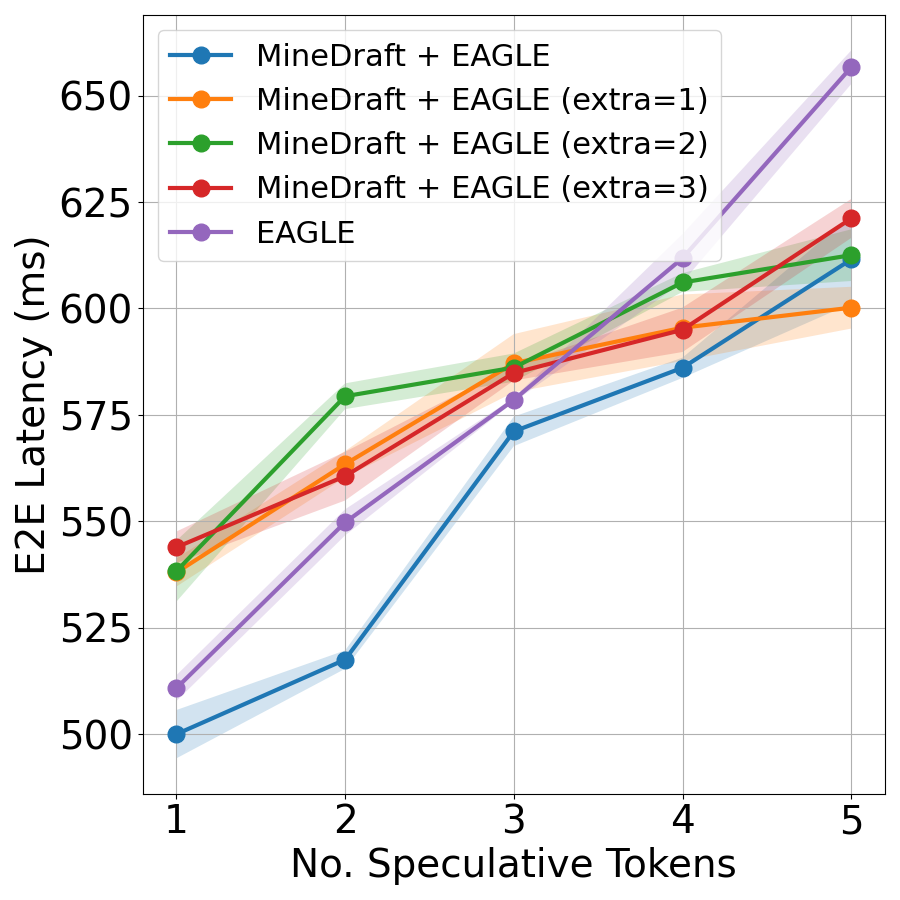
\includegraphics[width=0.23\linewidth]{results/Spec-Bench_vicuna-13b-v1_3_EAGLE-Vicuna-13B-v1_3_162_bs16_100pct_latency.png} &
        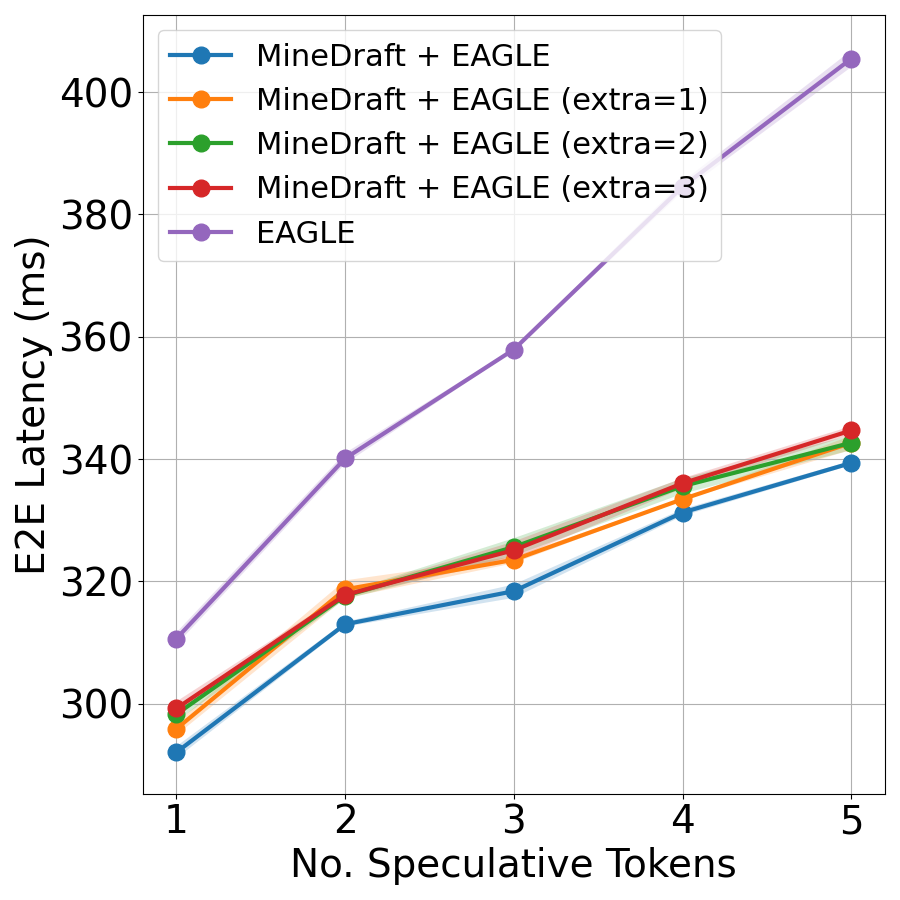
\includegraphics[width=0.23\linewidth]{results/Tough_vicuna-13b-v1_3_EAGLE-Vicuna-13B-v1_3_1000_bs16_100pct_latency.png} \\
        & \hspace{2mm}(i) \hspace{2mm} $\uparrow$ 4.95\%, $\Delta$ 15.95\% &
        \hspace{2mm}(j) \hspace{2mm} $\uparrow$ 4.98\%, $\Delta$ 14.37\% &
        \hspace{2mm}(k) \hspace{2mm} $\uparrow$ 2.12\%, $\Delta$ 8.60\% &
        \hspace{2mm}(l) \hspace{2mm} $\uparrow$ 5.99\%, $\Delta$ 16.30\% \\
    \end{tabular}}
    \caption{End-to-End Latency (ms) comparison across model settings 5--7. $\uparrow$ indicates the average improvement over the best baseline method. $\Delta$ indicates the maximum average gap between \alg{} and standard SD or EAGLE.
    }
    \label{fig:e2elatencty-strategy}
\end{figure*}


\begin{figure*}[!ht]
    \centering
    \setlength{\tabcolsep}{1pt} 
    \resizebox{0.99\linewidth}{!}{
    \begin{tabular}{ccccc}
        & \hspace{8mm}\textbf{Arena} & \hspace{8mm}\textbf{ShareGPT} & \hspace{8mm}\textbf{Spec-Bench}  & \hspace{8mm}\textbf{Tough}\\

        \rotatebox{90}{\parbox{3.5cm}{\centering \hspace{8mm}\textbf{Throughput}}} & 
        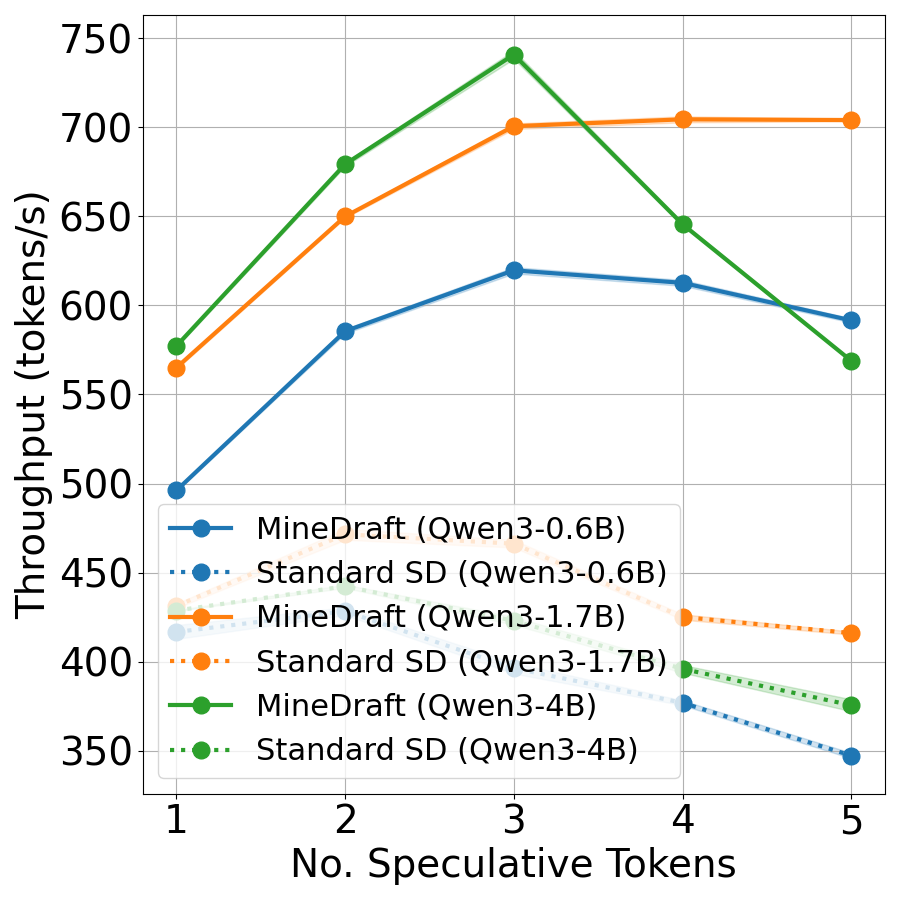
\includegraphics[width=0.23\linewidth]{results/Arena_Qwen3-32B_1000_bs16_100pct_gen_throughput.png} &
        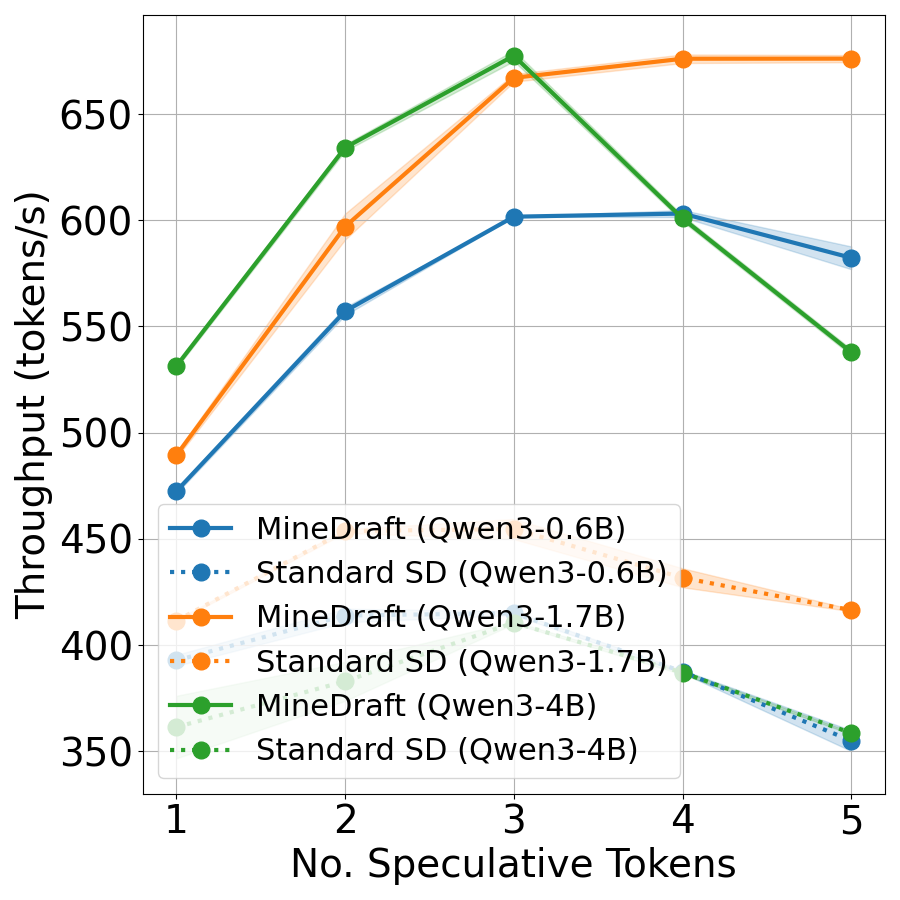
\includegraphics[width=0.23\linewidth]{results/ShareGPT_Qwen3-32B_1000_bs16_100pct_gen_throughput.png} &
        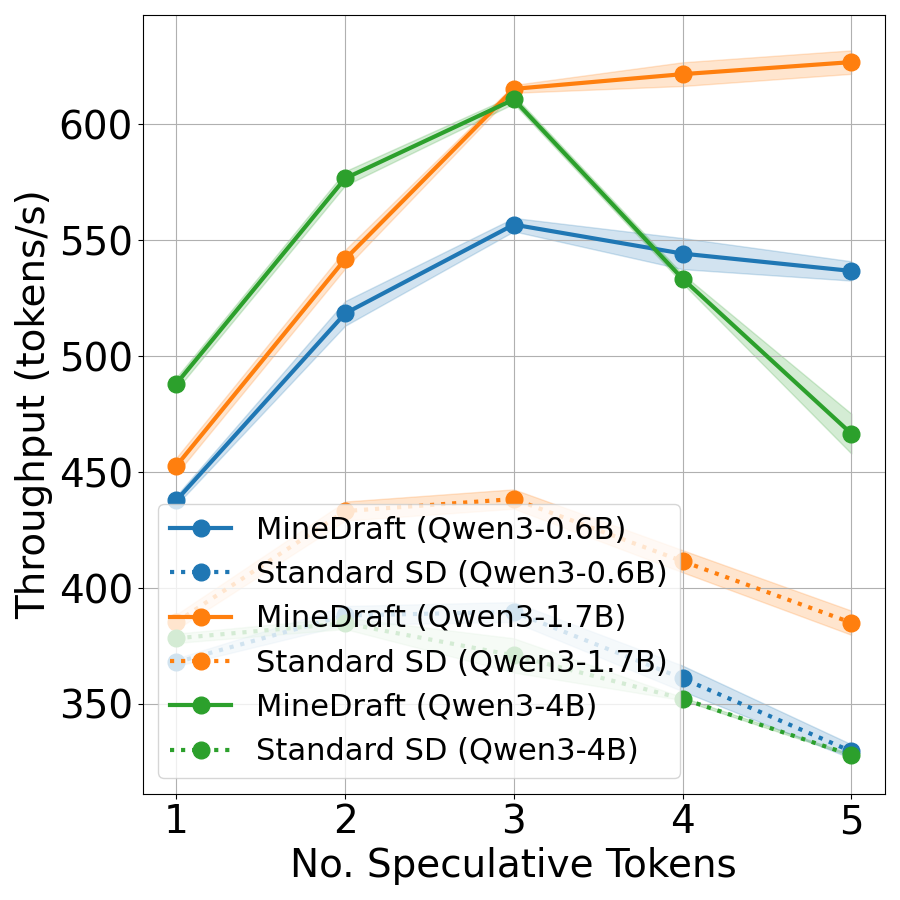
\includegraphics[width=0.23\linewidth]{results/Spec-Bench_Qwen3-32B_161_bs16_100pct_gen_throughput.png} &
        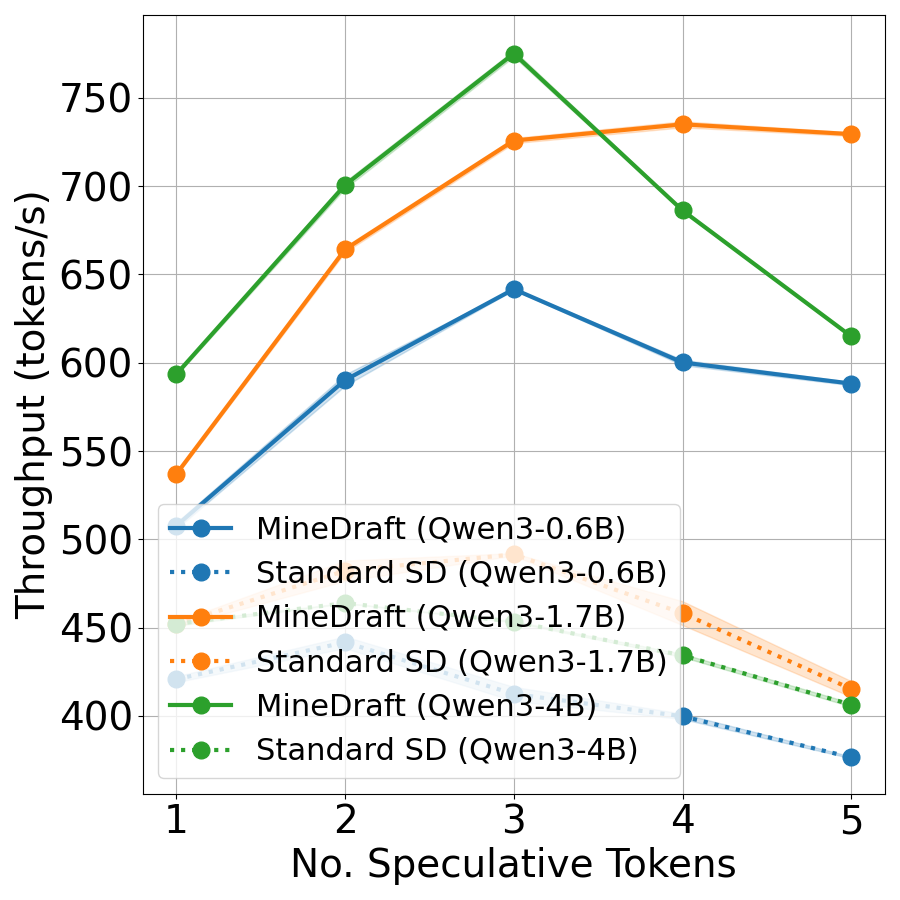
\includegraphics[width=0.23\linewidth]{results/Tough_Qwen3-32B_1000_bs16_100pct_gen_throughput.png} \\

        \rotatebox{90}{\parbox{3.5cm}{\centering \hspace{8mm}\textbf{E2EL}}} &
        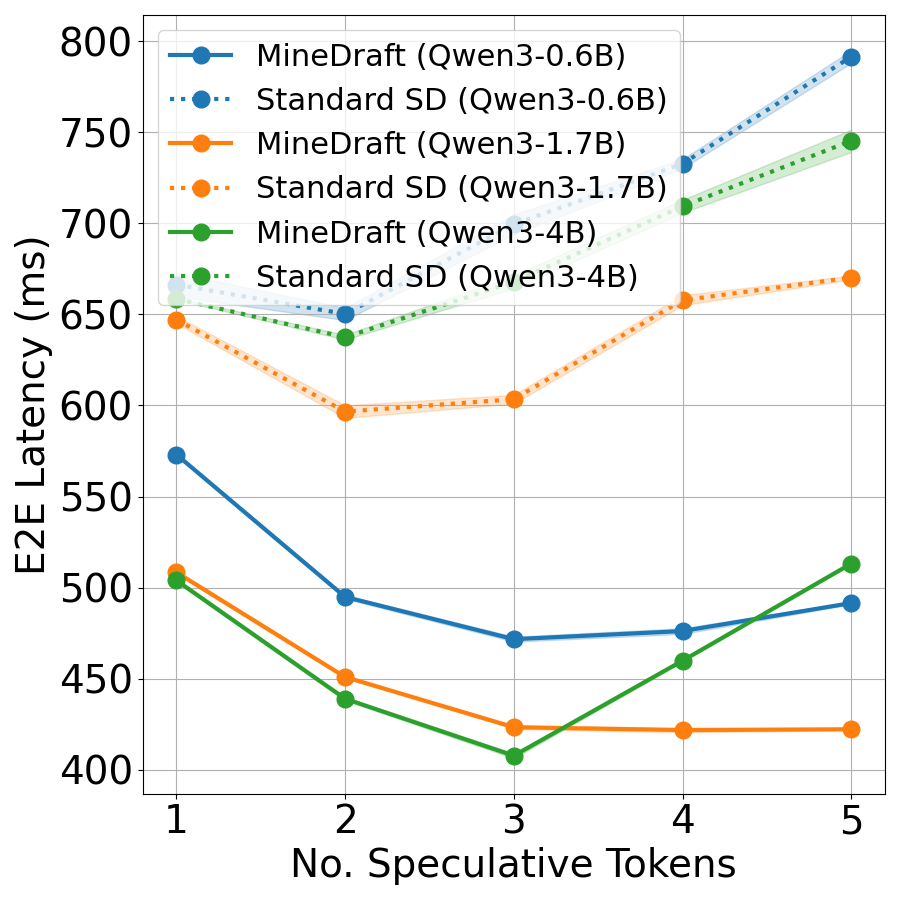
\includegraphics[width=0.23\linewidth]{results/Arena_Qwen3-32B_1000_bs16_100pct_latency.png} &
        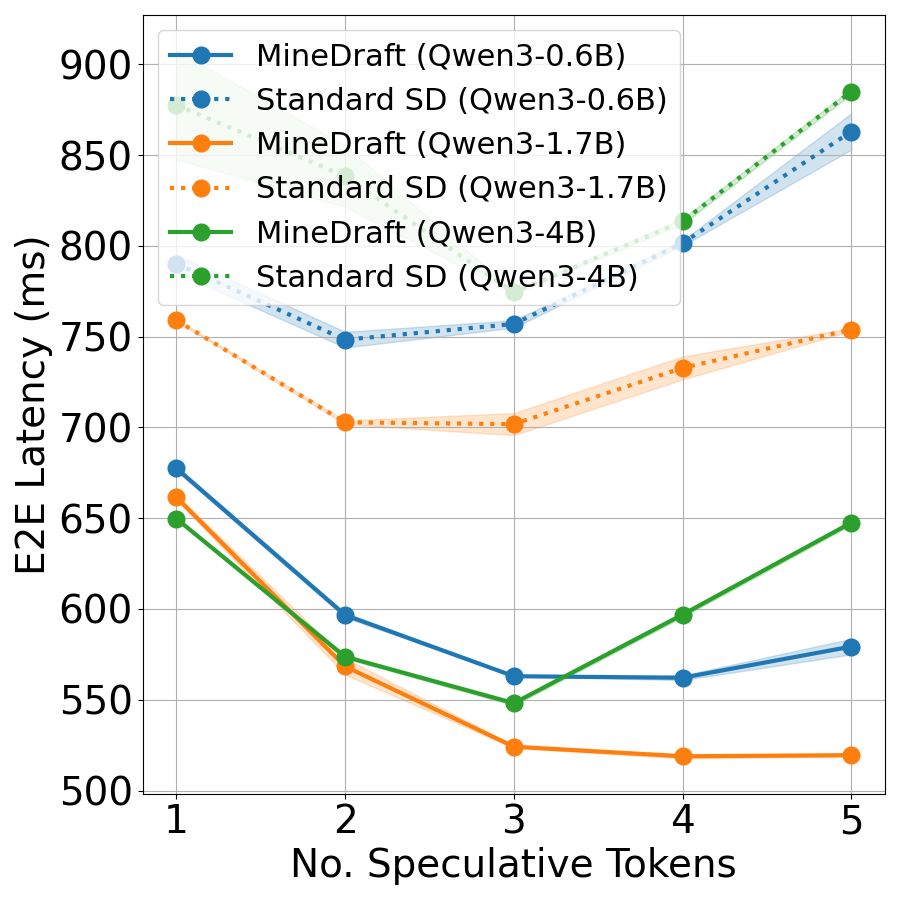
\includegraphics[width=0.23\linewidth]{results/ShareGPT_Qwen3-32B_1000_bs16_100pct_latency.png} &
        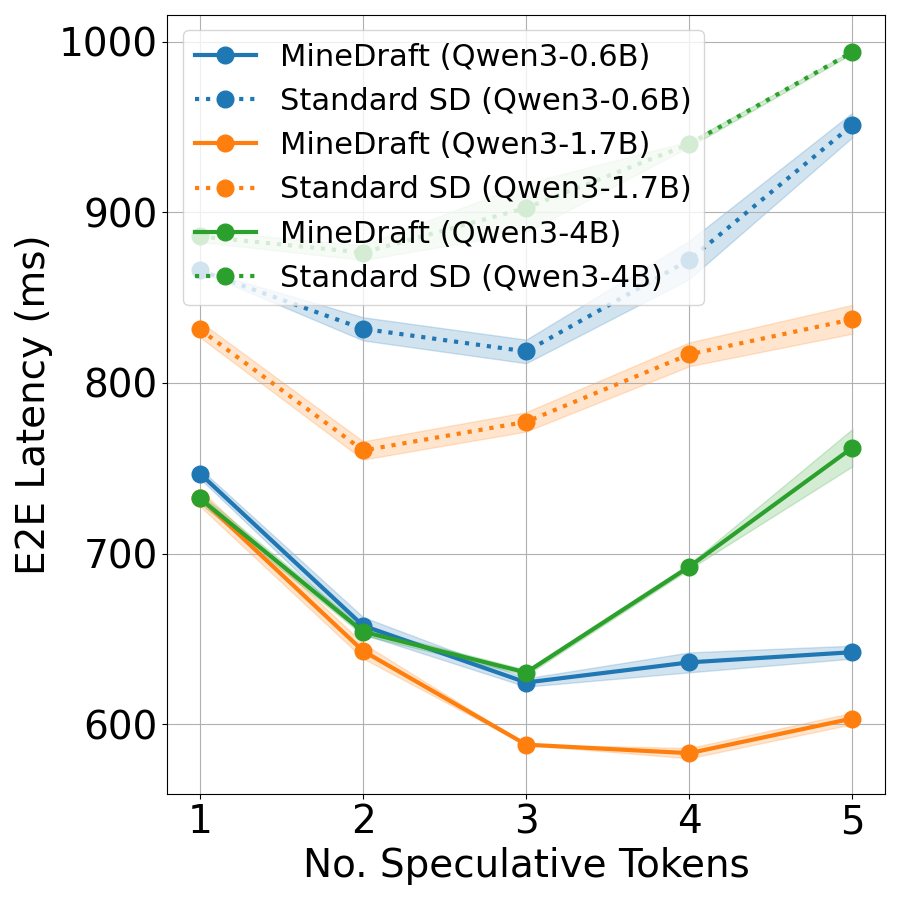
\includegraphics[width=0.23\linewidth]{results/Spec-Bench_Qwen3-32B_161_bs16_100pct_latency.png} &
        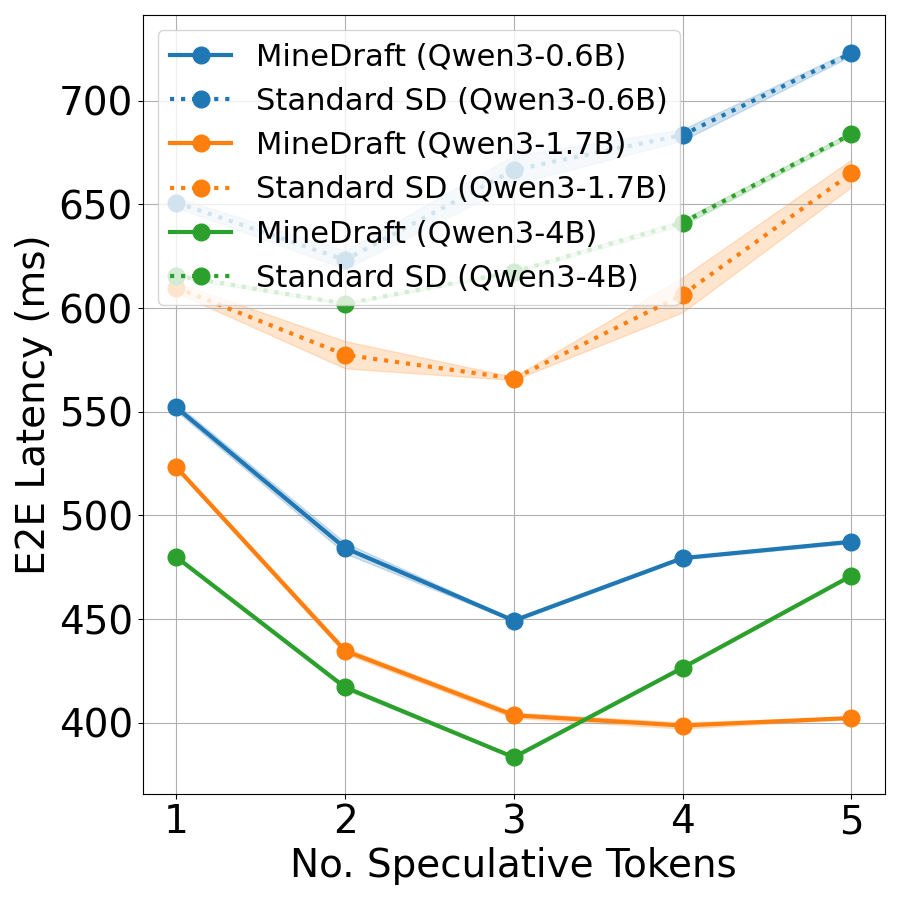
\includegraphics[width=0.23\linewidth]{results/Tough_Qwen3-32B_1000_bs16_100pct_latency.png} 
    \end{tabular}}
    \caption{Comparisons for various draft models paired with Qwen3-32B using \alg{}.
    }
    \label{fig:qwen3-32b-draft-models}
\end{figure*}


\begin{figure*}[!ht]
    \centering
    \setlength{\tabcolsep}{1pt} 
    \resizebox{0.99\linewidth}{!}{
    \begin{tabular}{ccccc}
        & \hspace{8mm}\textbf{Arena} & \hspace{8mm}\textbf{ShareGPT} & \hspace{8mm}\textbf{Spec-Bench}  & \hspace{8mm}\textbf{Tough}\\
        
        \rotatebox{90}{\parbox{3.5cm}{\centering \hspace{8mm}\textbf{Qwen3~32B-0.6B}}} & 
        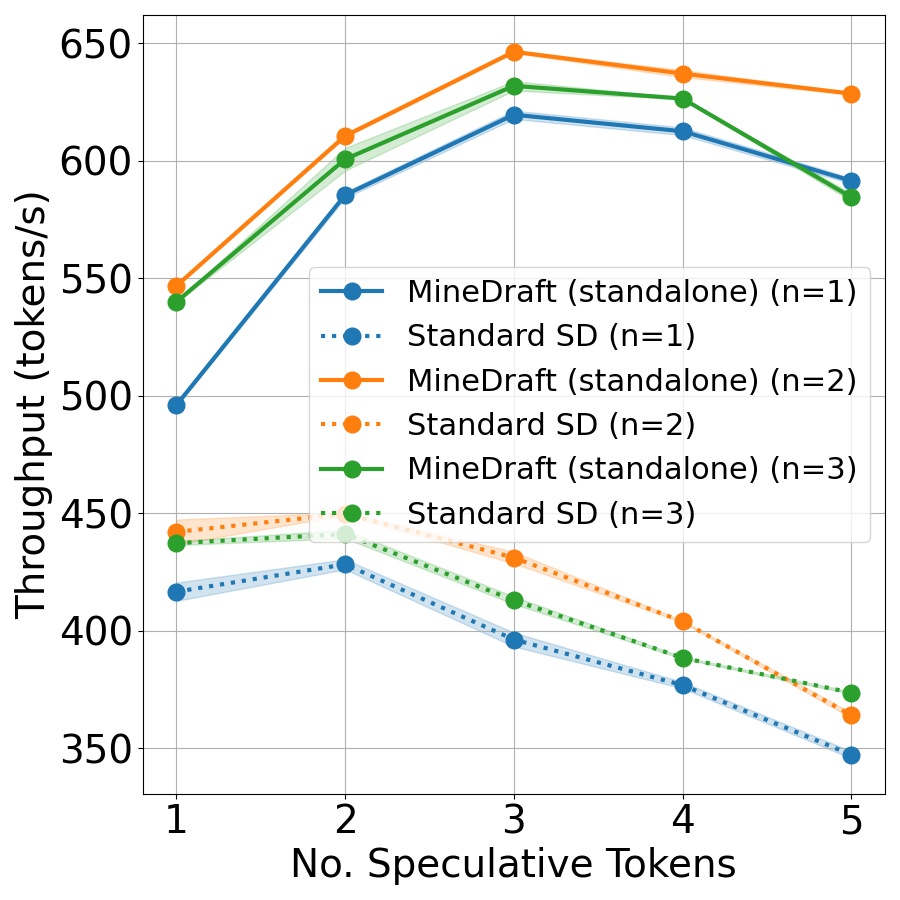
\includegraphics[width=0.23\linewidth]{results/Arena_Qwen3-32B_Qwen3-0_6B_1000_bs16_100pct_gen_throughput_vs_n.png} &
        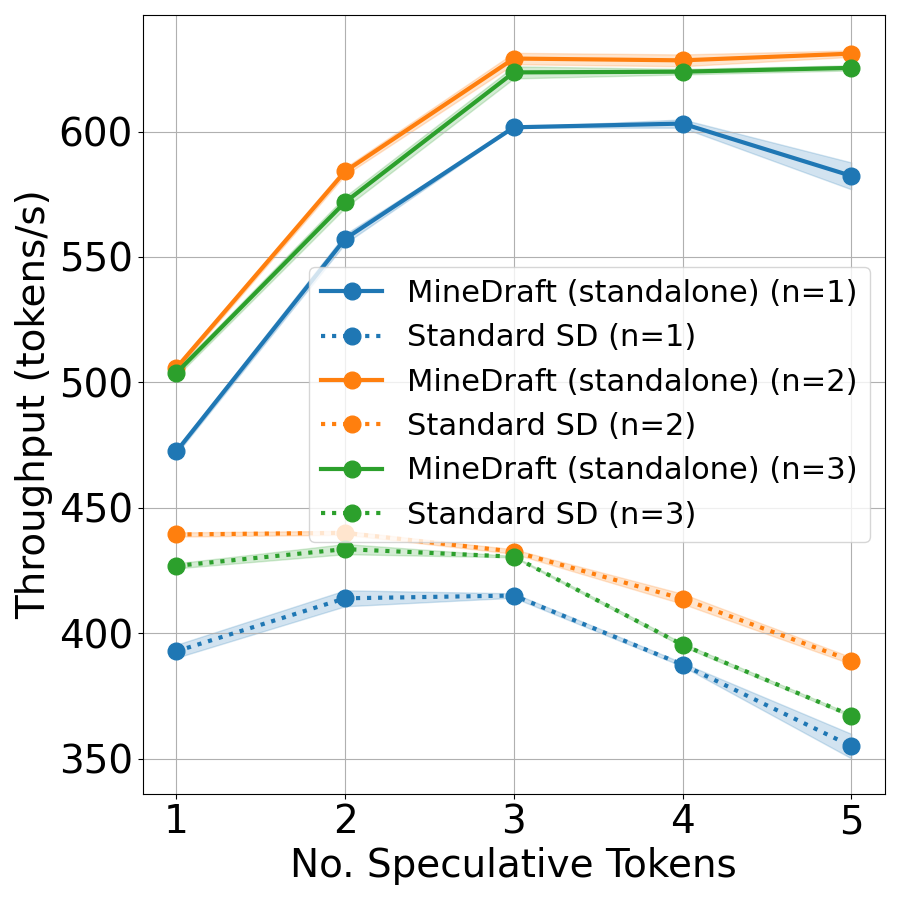
\includegraphics[width=0.23\linewidth]{results/ShareGPT_Qwen3-32B_Qwen3-0_6B_1000_bs16_100pct_gen_throughput_vs_n.png} &
        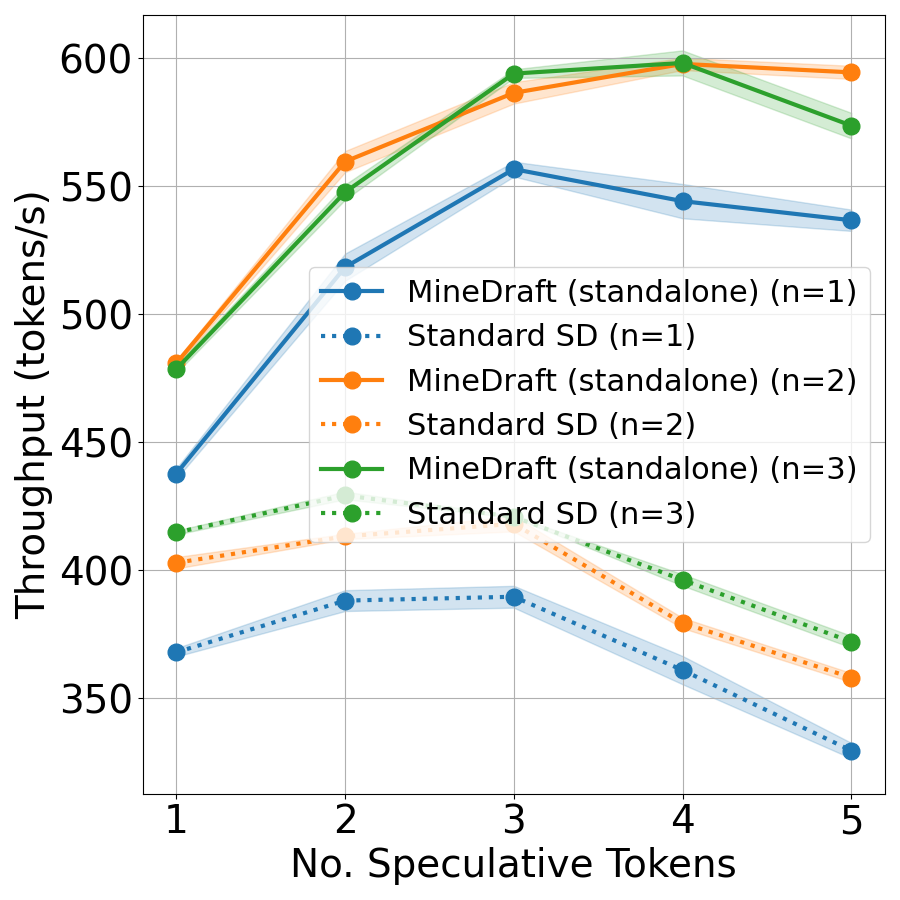
\includegraphics[width=0.23\linewidth]{results/Spec-Bench_Qwen3-32B_Qwen3-0_6B_161_bs16_100pct_gen_throughput_vs_n.png} &
        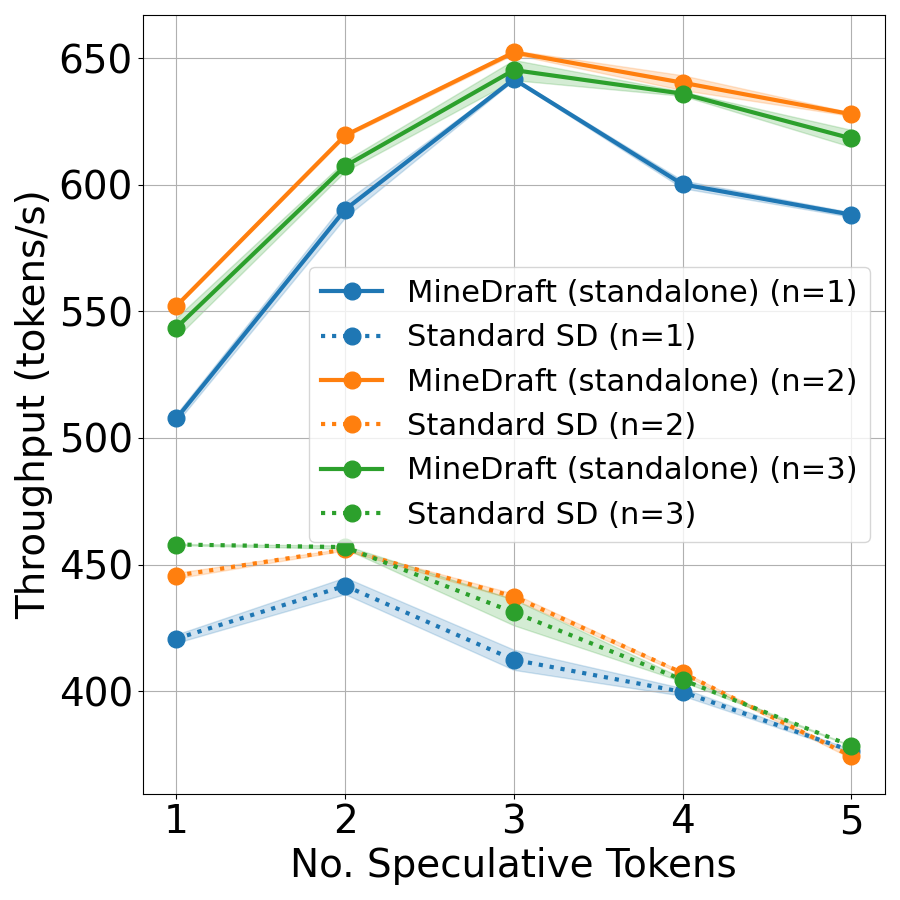
\includegraphics[width=0.23\linewidth]{results/Tough_Qwen3-32B_Qwen3-0_6B_1000_bs16_100pct_gen_throughput_vs_n.png} \\
    
    \end{tabular}}
    \caption{Throughput comparison against standard SD across various $n$ on model setting 1.
    }
    \label{fig:throughput-n}
\end{figure*}


\begin{figure*}[!ht]
    \centering
    \setlength{\tabcolsep}{1pt} 
    \resizebox{0.99\linewidth}{!}{
    \begin{tabular}{ccccc}
        & \hspace{8mm}\textbf{Arena} & \hspace{8mm}\textbf{ShareGPT} & \hspace{8mm}\textbf{Spec-Bench}  & \hspace{8mm}\textbf{Tough}\\
        
        \rotatebox{90}{\parbox{3.5cm}{\centering \hspace{8mm}\textbf{Qwen3~32B-0.6B}}} & 
        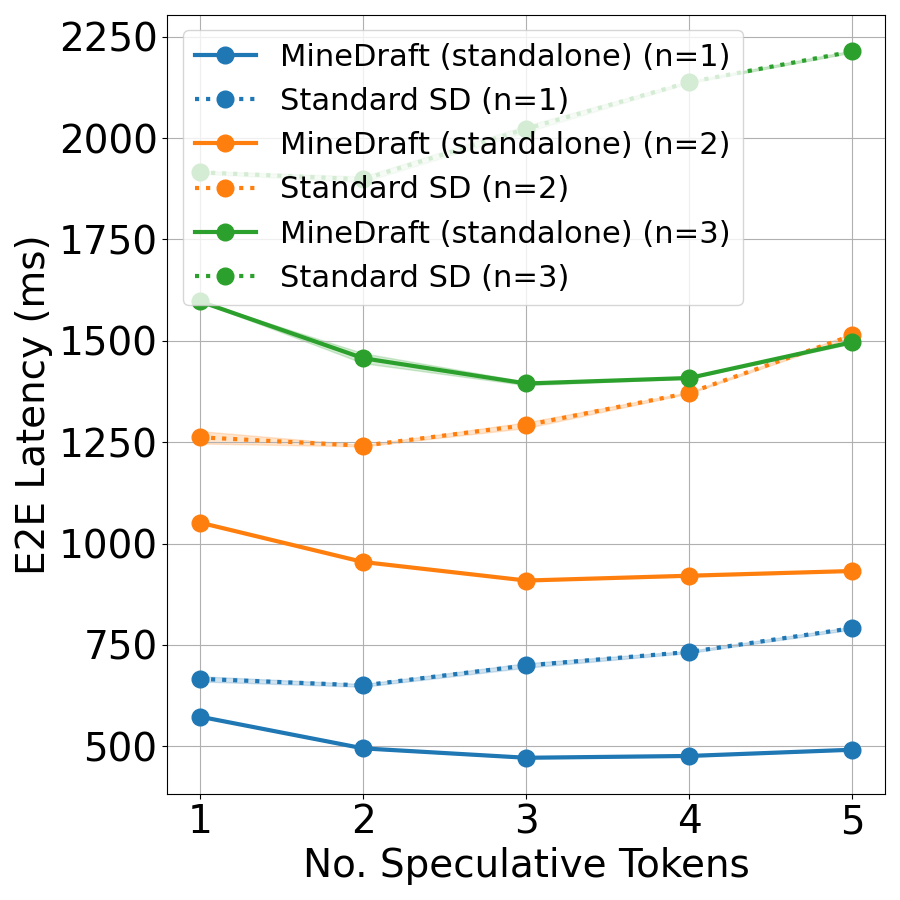
\includegraphics[width=0.23\linewidth]{results/Arena_Qwen3-32B_Qwen3-0_6B_1000_bs16_100pct_latency_vs_n.png} &
        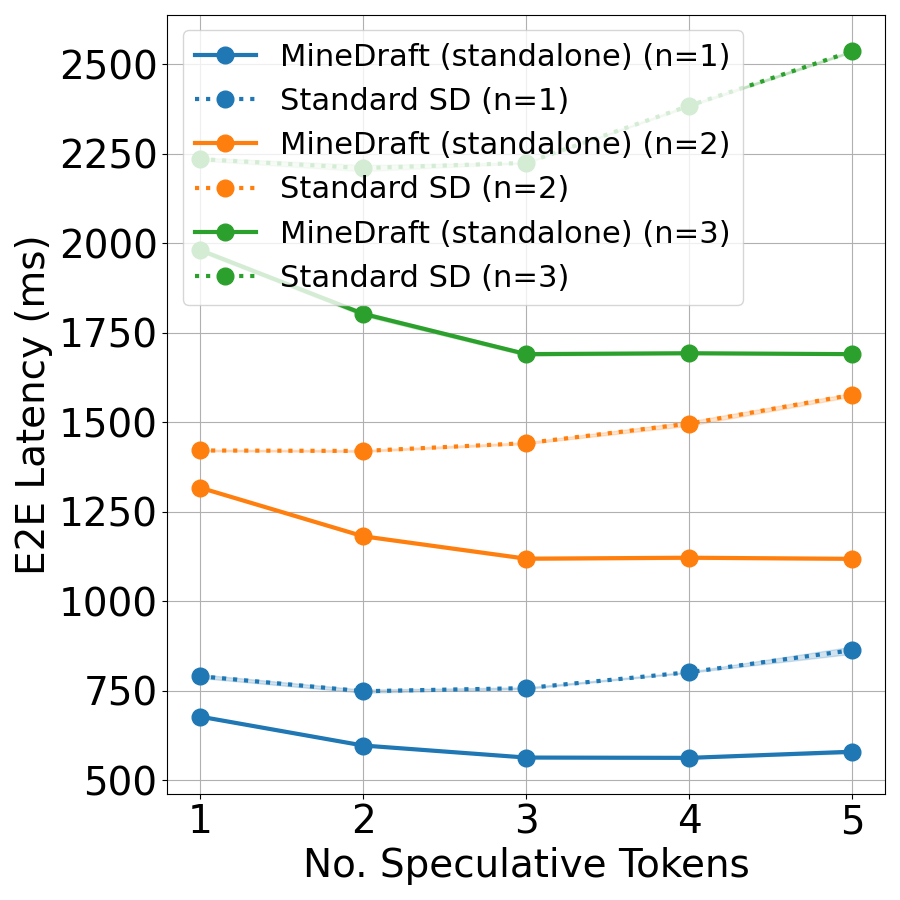
\includegraphics[width=0.23\linewidth]{results/ShareGPT_Qwen3-32B_Qwen3-0_6B_1000_bs16_100pct_latency_vs_n.png} &
        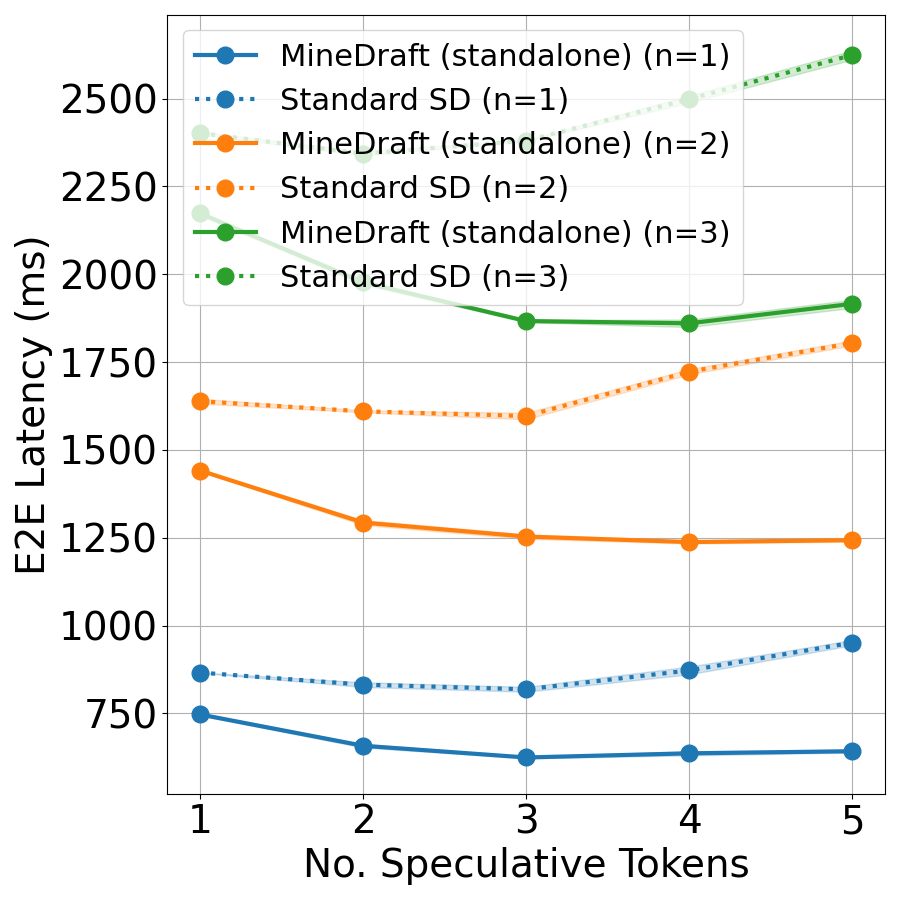
\includegraphics[width=0.23\linewidth]{results/Spec-Bench_Qwen3-32B_Qwen3-0_6B_161_bs16_100pct_latency_vs_n.png} &
        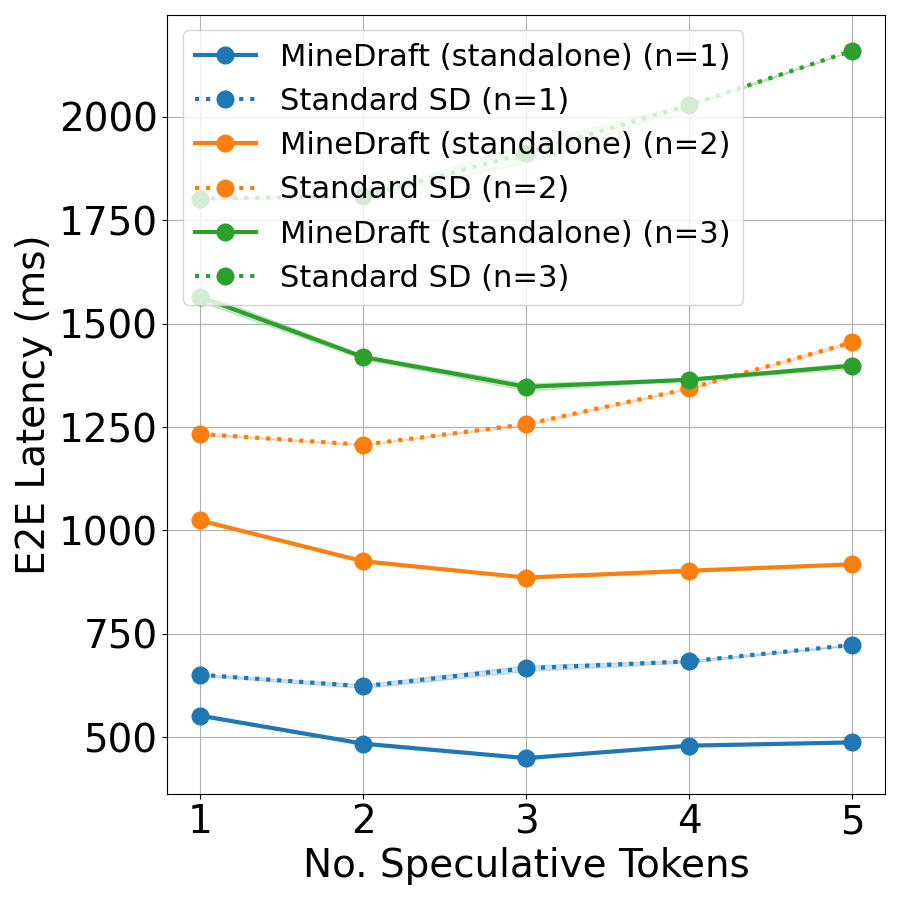
\includegraphics[width=0.23\linewidth]{results/Tough_Qwen3-32B_Qwen3-0_6B_1000_bs16_100pct_latency_vs_n.png} \\
    
    \end{tabular}}
    \caption{End-to-End Latency (ms) comparison against standard SD across various $n$ on model setting 1.
    }
    \label{fig:e2elatencty-n}
\end{figure*}


\begin{figure*}[!ht]
    \centering
    \setlength{\tabcolsep}{1pt} 
    \resizebox{0.99\linewidth}{!}{
    \begin{tabular}{ccccc}
        & \hspace{8mm}\textbf{Arena} & \hspace{8mm}\textbf{ShareGPT} & \hspace{8mm}\textbf{Spec-Bench}  & \hspace{8mm}\textbf{Tough}\\
        
        \rotatebox{90}{\parbox{3.5cm}{\centering \hspace{8mm}\textbf{Qwen3~32B-0.6B}}} & 
        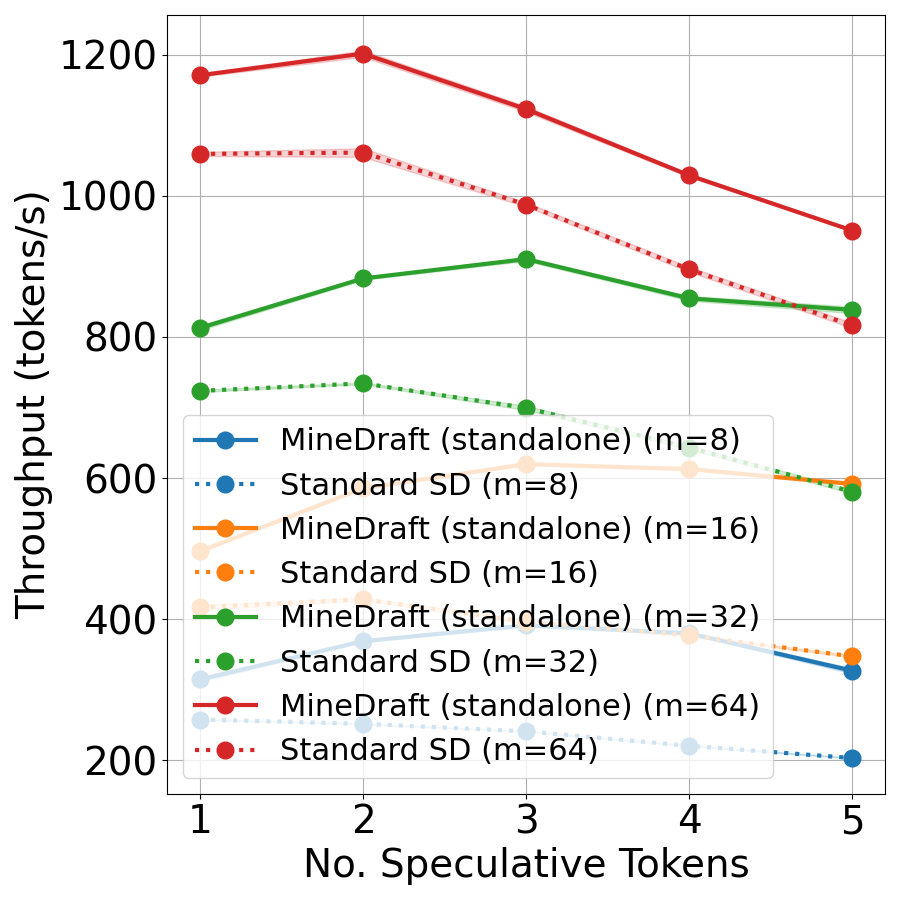
\includegraphics[width=0.23\linewidth]{results/Arena_Qwen3-32B_Qwen3-0_6B_1000_100pct_gen_throughput_vs_m.png} &
        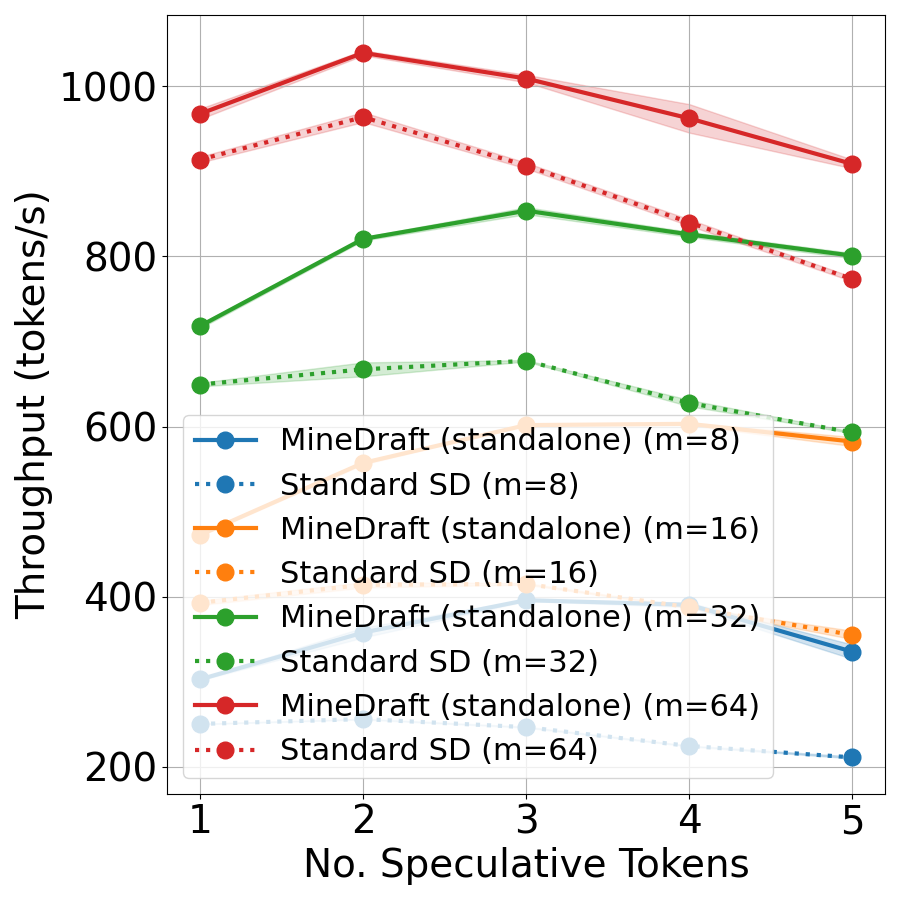
\includegraphics[width=0.23\linewidth]{results/ShareGPT_Qwen3-32B_Qwen3-0_6B_1000_100pct_gen_throughput_vs_m.png} &
        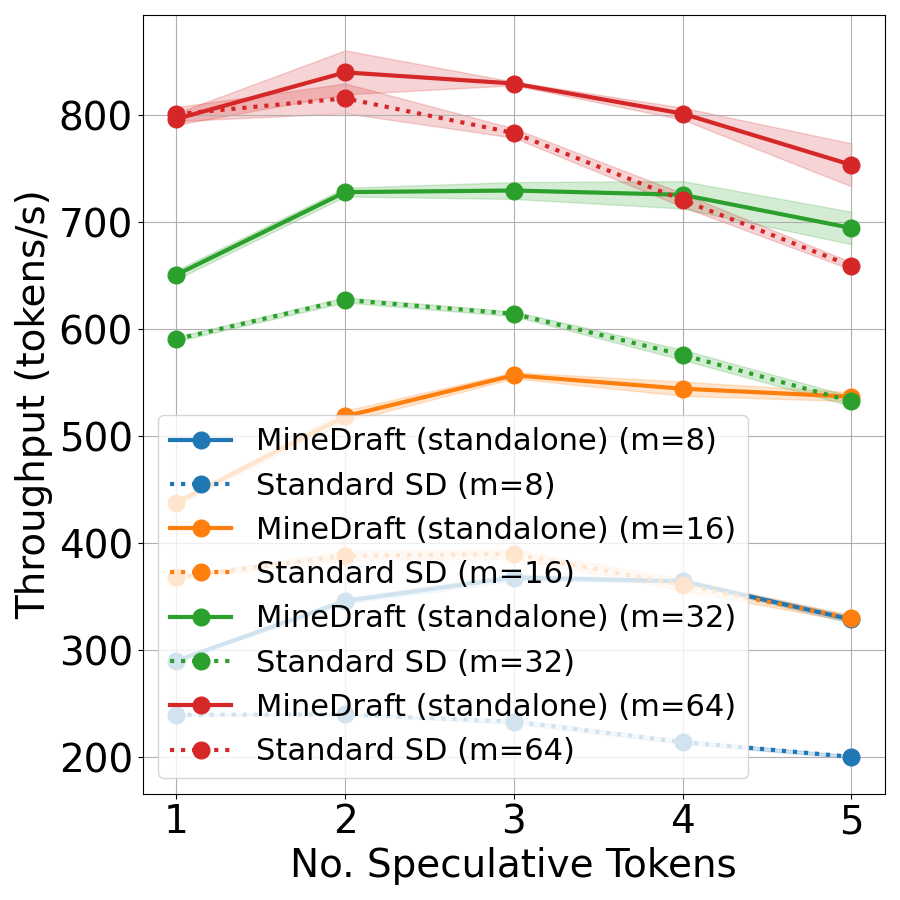
\includegraphics[width=0.23\linewidth]{results/Spec-Bench_Qwen3-32B_Qwen3-0_6B_161_100pct_gen_throughput_vs_m.png} &
        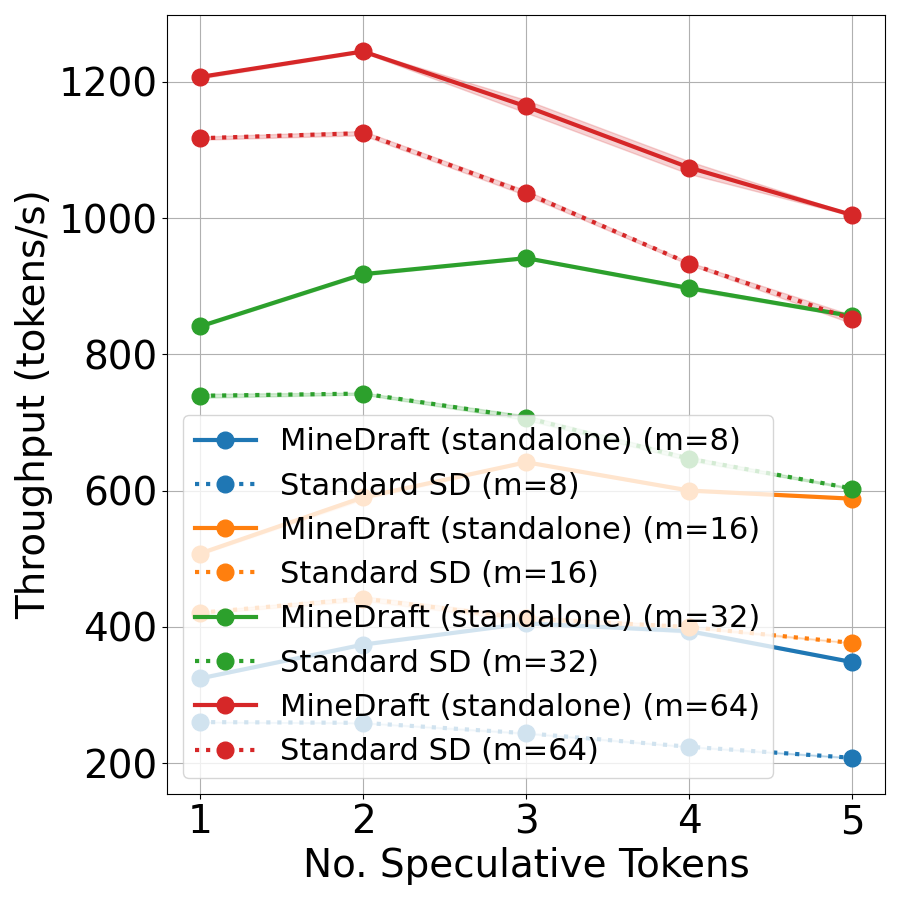
\includegraphics[width=0.23\linewidth]{results/Tough_Qwen3-32B_Qwen3-0_6B_1000_100pct_gen_throughput_vs_m.png} \\

    \end{tabular}}
    \caption{Throughput comparison against standard SD across various $m$ (batch size) on model setting 1.
    }
    \label{fig:throughput-bs}
\end{figure*}


\begin{figure*}[!ht]
    \centering
    \setlength{\tabcolsep}{1pt} 
    \resizebox{0.99\linewidth}{!}{
    \begin{tabular}{ccccc}
        & \hspace{8mm}\textbf{Arena} & \hspace{8mm}\textbf{ShareGPT} & \hspace{8mm}\textbf{Spec-Bench}  & \hspace{8mm}\textbf{Tough}\\
        
        \rotatebox{90}{\parbox{3.5cm}{\centering \hspace{8mm}\textbf{Qwen3~32B-0.6B}}} & 
        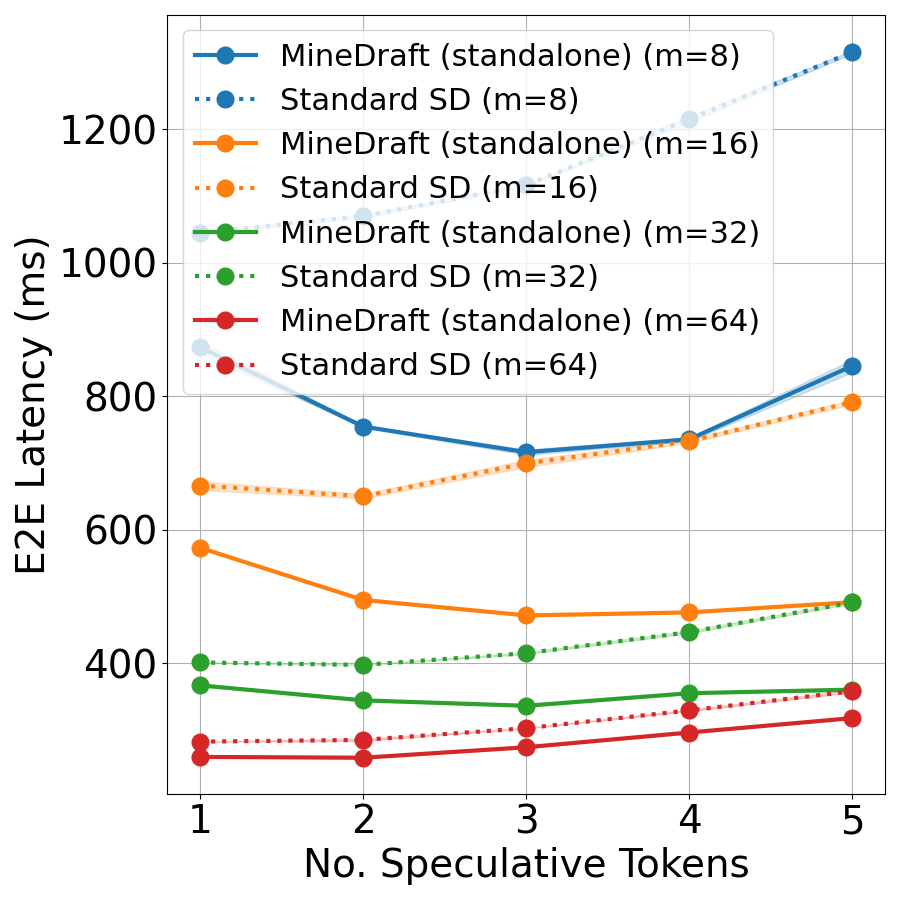
\includegraphics[width=0.23\linewidth]{results/Arena_Qwen3-32B_Qwen3-0_6B_1000_100pct_latency_vs_m.png} &
        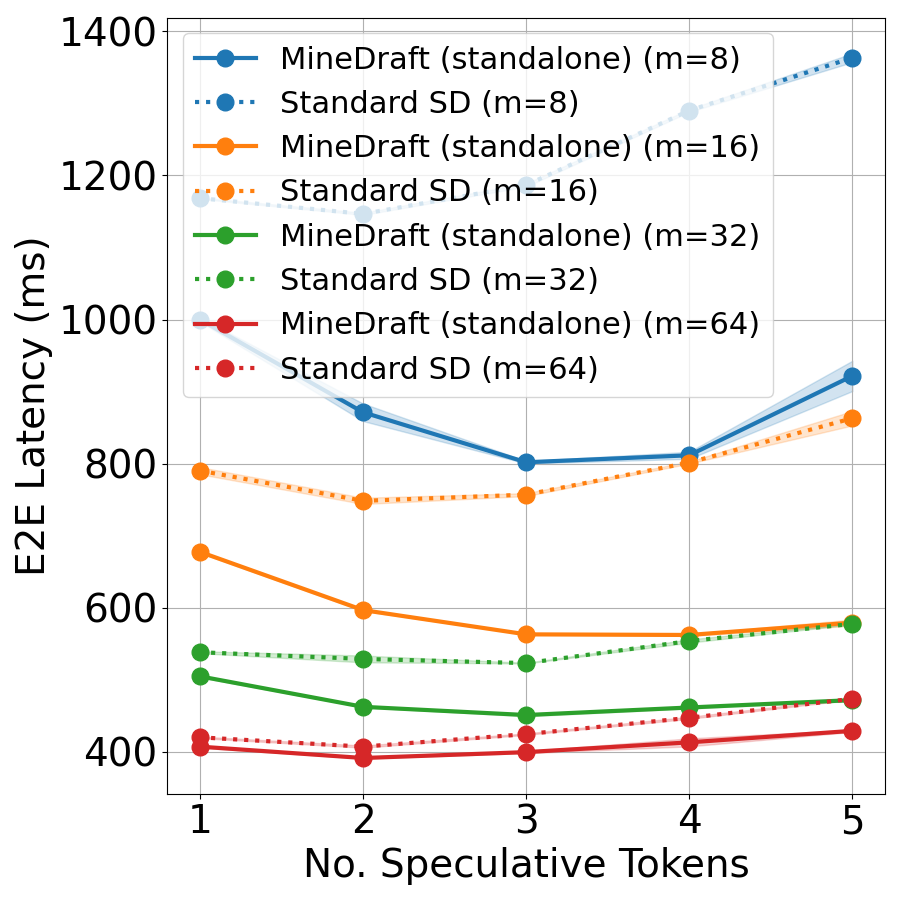
\includegraphics[width=0.23\linewidth]{results/ShareGPT_Qwen3-32B_Qwen3-0_6B_1000_100pct_latency_vs_m.png} &
        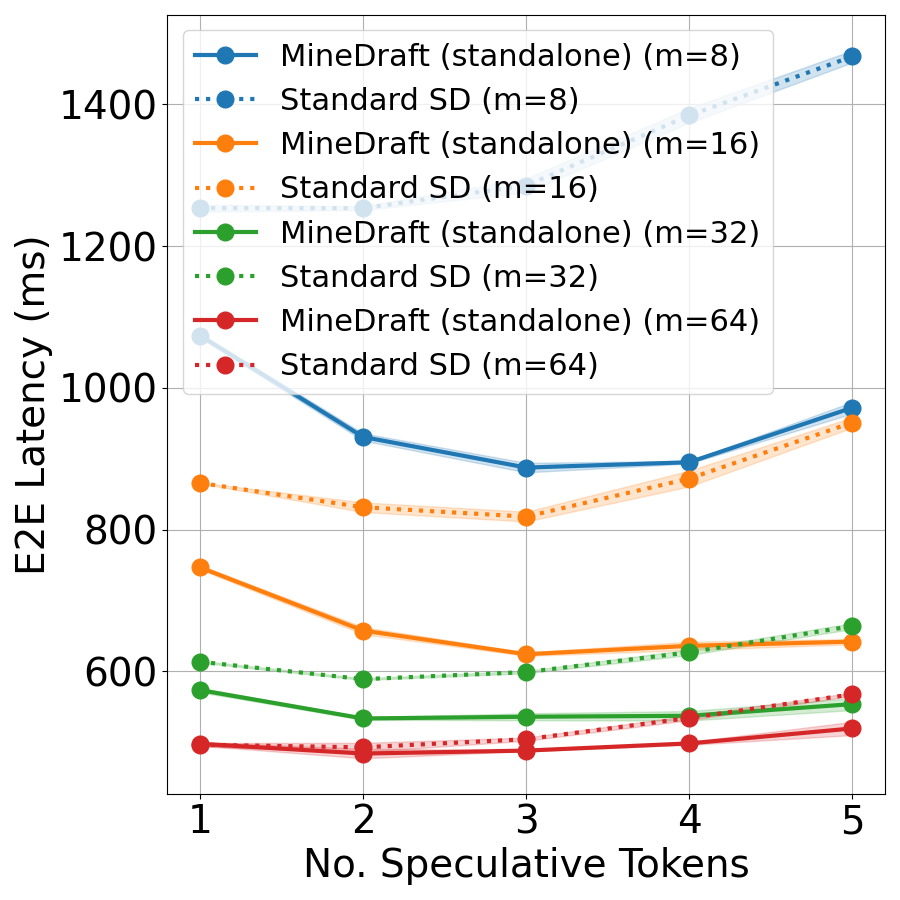
\includegraphics[width=0.23\linewidth]{results/Spec-Bench_Qwen3-32B_Qwen3-0_6B_161_100pct_latency_vs_m.png} &
        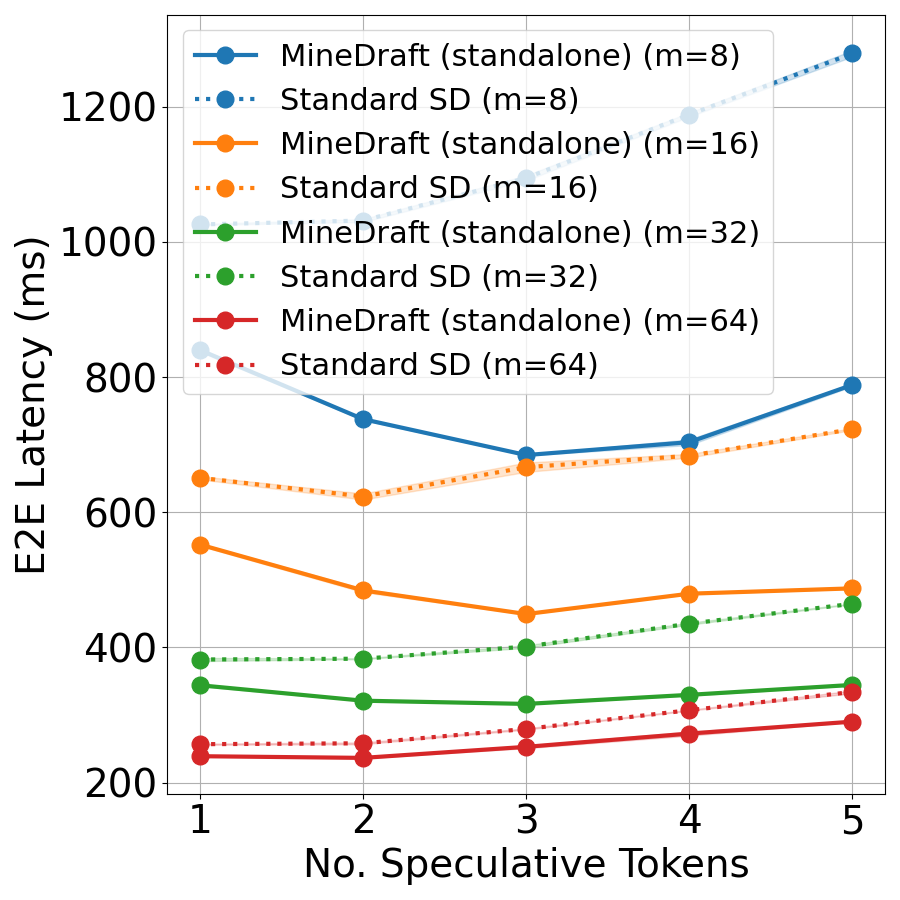
\includegraphics[width=0.23\linewidth]{results/Tough_Qwen3-32B_Qwen3-0_6B_1000_100pct_latency_vs_m.png} \\

    \end{tabular}}
    \caption{End-to-End Latency (ms) comparison against standard SD across various $m$ (batch size) on model setting 1.
    }
    \label{fig:e2elatencty-bs}
\end{figure*}


\begin{figure*}[!ht]
    \centering
    \setlength{\tabcolsep}{1pt}
    \resizebox{0.99\linewidth}{!}{
    \begin{tabular}{ccccc}
        & \hspace{8mm}\textbf{Arena} & \hspace{8mm}\textbf{ShareGPT} & \hspace{8mm}\textbf{Spec-Bench}  & \hspace{8mm}\textbf{Tough}\\
        
        \rotatebox{90}{\parbox{3.5cm}{\centering \hspace{8mm}\textbf{Qwen3~32B-0.6B}}} & 
        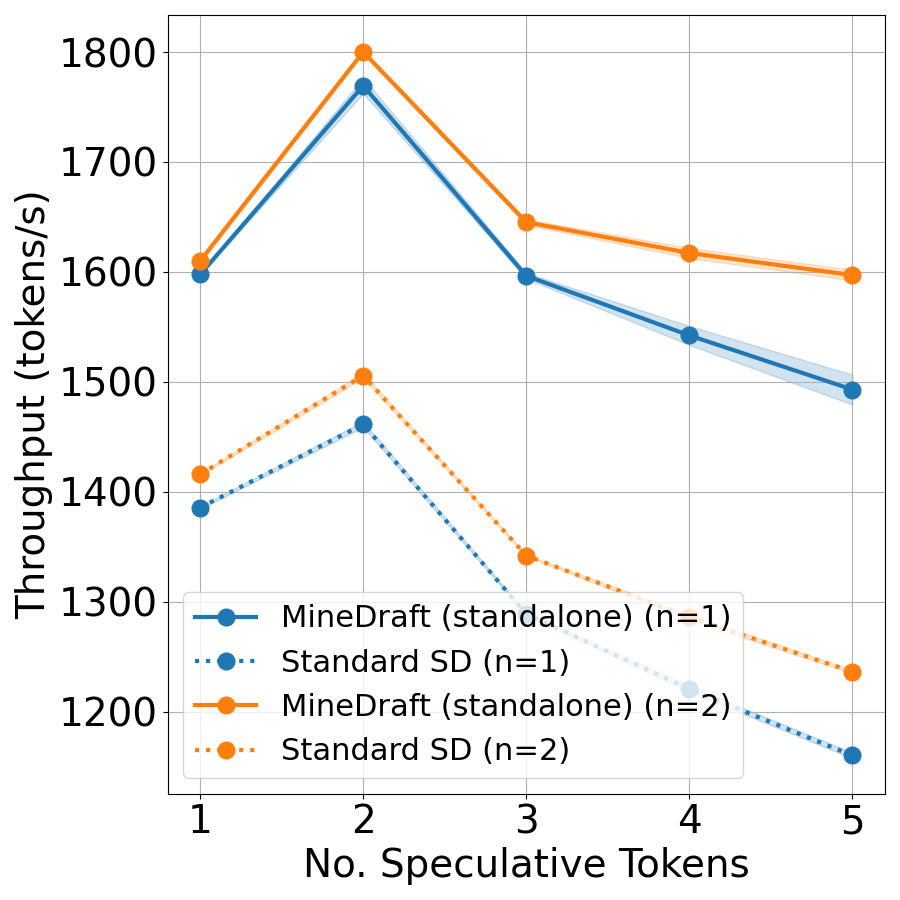
\includegraphics[width=0.23\linewidth]{results/Arena_Meta-Llama-3_3-70B-Instruct-AWQ-INT4_Llama-3_1-8B-Instruct_1000_bs64_100pct_gen_throughput_vs_n.png} &
        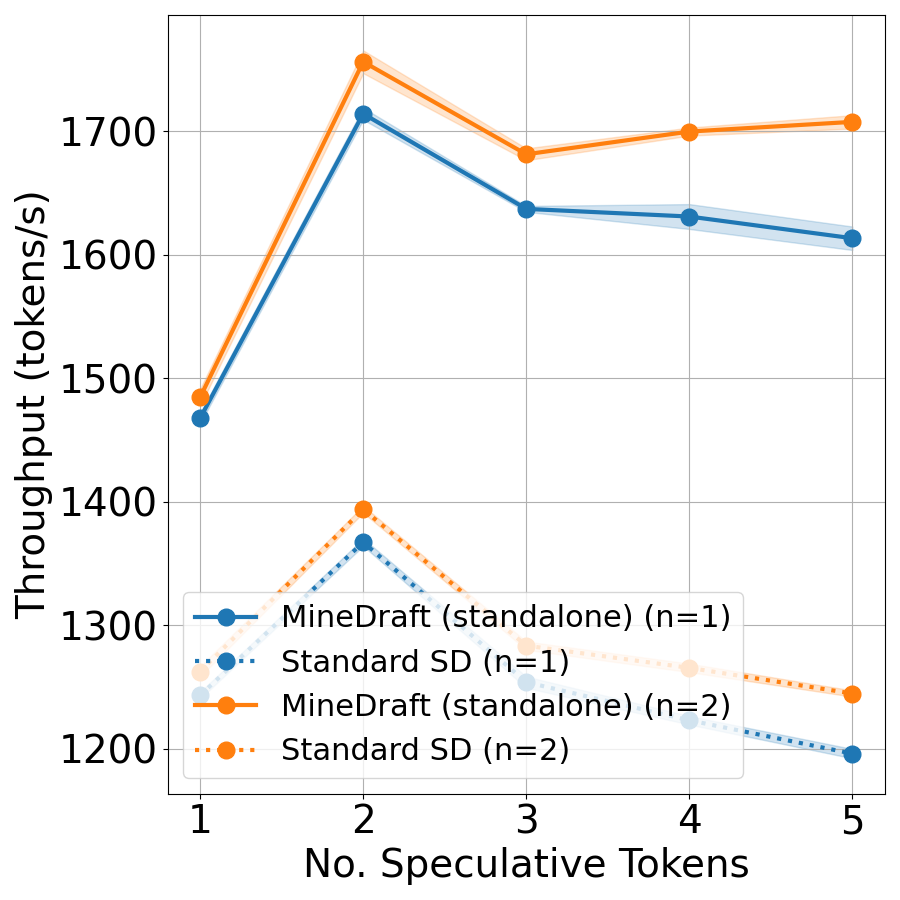
\includegraphics[width=0.23\linewidth]{results/ShareGPT_Meta-Llama-3_3-70B-Instruct-AWQ-INT4_Llama-3_1-8B-Instruct_1000_bs64_100pct_gen_throughput_vs_n.png} &
        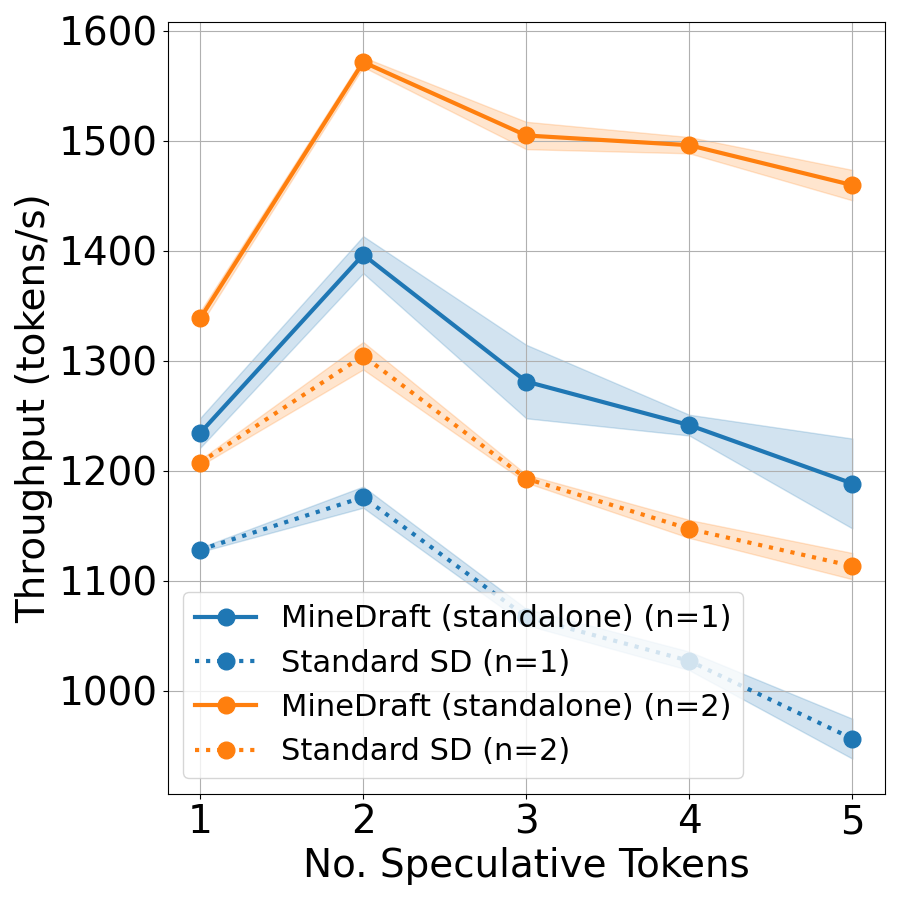
\includegraphics[width=0.23\linewidth]{results/Spec-Bench_Meta-Llama-3_3-70B-Instruct-AWQ-INT4_Llama-3_1-8B-Instruct_160_bs64_100pct_gen_throughput_vs_n.png} &
        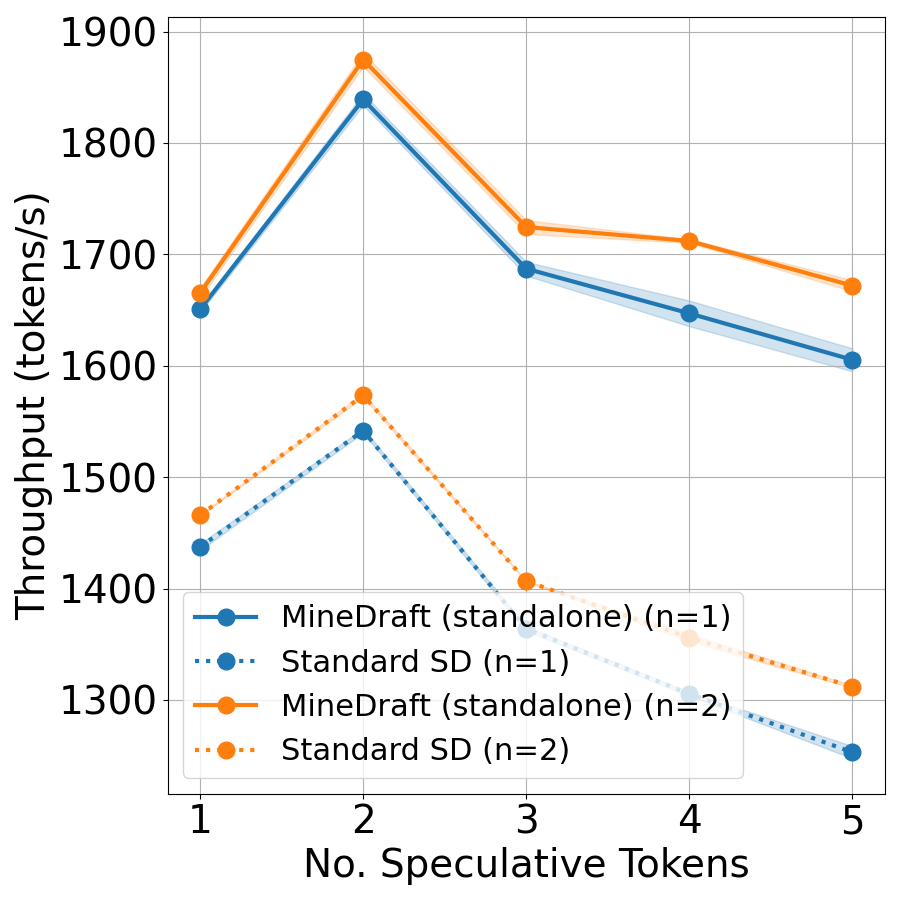
\includegraphics[width=0.23\linewidth]{results/Tough_Meta-Llama-3_3-70B-Instruct-AWQ-INT4_Llama-3_1-8B-Instruct_1000_bs64_100pct_gen_throughput_vs_n.png} \\

    \end{tabular}}
    \caption{Throughput comparison against standard SD across various $n$ on model setting 5.
    }
    \label{fig:throughput-n-llama}
\end{figure*}


\begin{figure*}[!ht]
    \centering
    \setlength{\tabcolsep}{1pt} 
    \resizebox{0.99\linewidth}{!}{
    \begin{tabular}{ccccc}
        & \hspace{8mm}\textbf{Arena} & \hspace{8mm}\textbf{ShareGPT} & \hspace{8mm}\textbf{Spec-Bench}  & \hspace{8mm}\textbf{Tough}\\
        
        \rotatebox{90}{\parbox{3.5cm}{\centering \hspace{8mm}\textbf{Qwen3~32B-0.6B}}} & 
        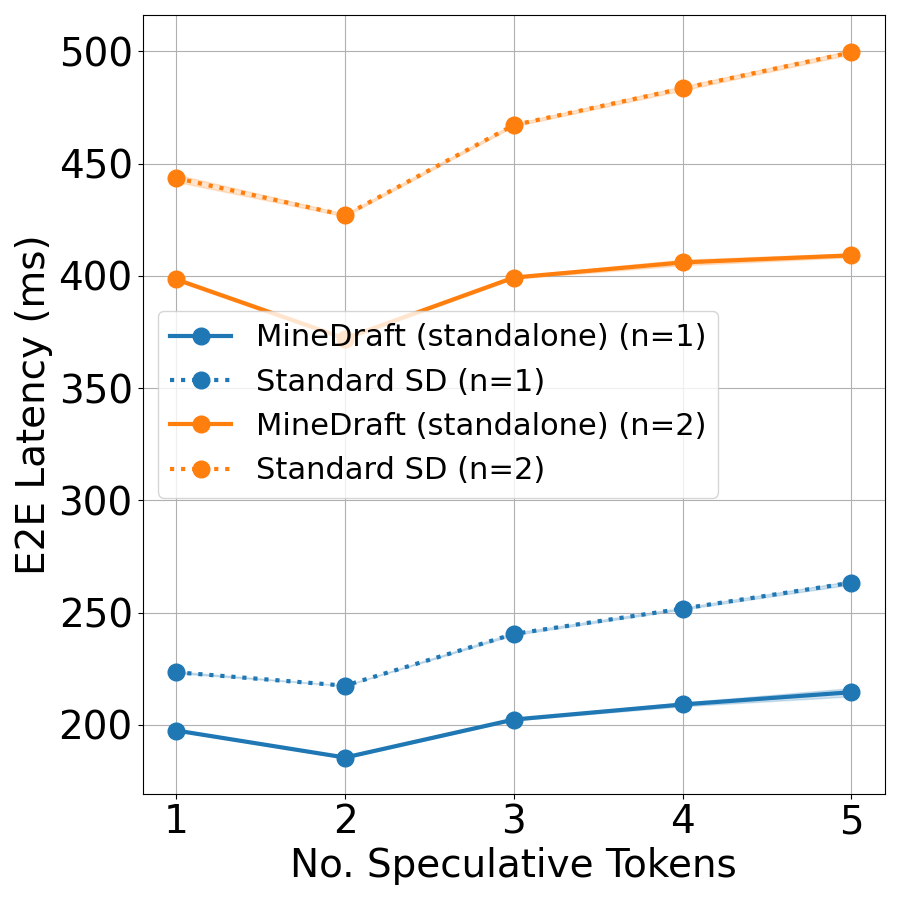
\includegraphics[width=0.23\linewidth]{results/Arena_Meta-Llama-3_3-70B-Instruct-AWQ-INT4_Llama-3_1-8B-Instruct_1000_bs64_100pct_latency_vs_n.png} &
        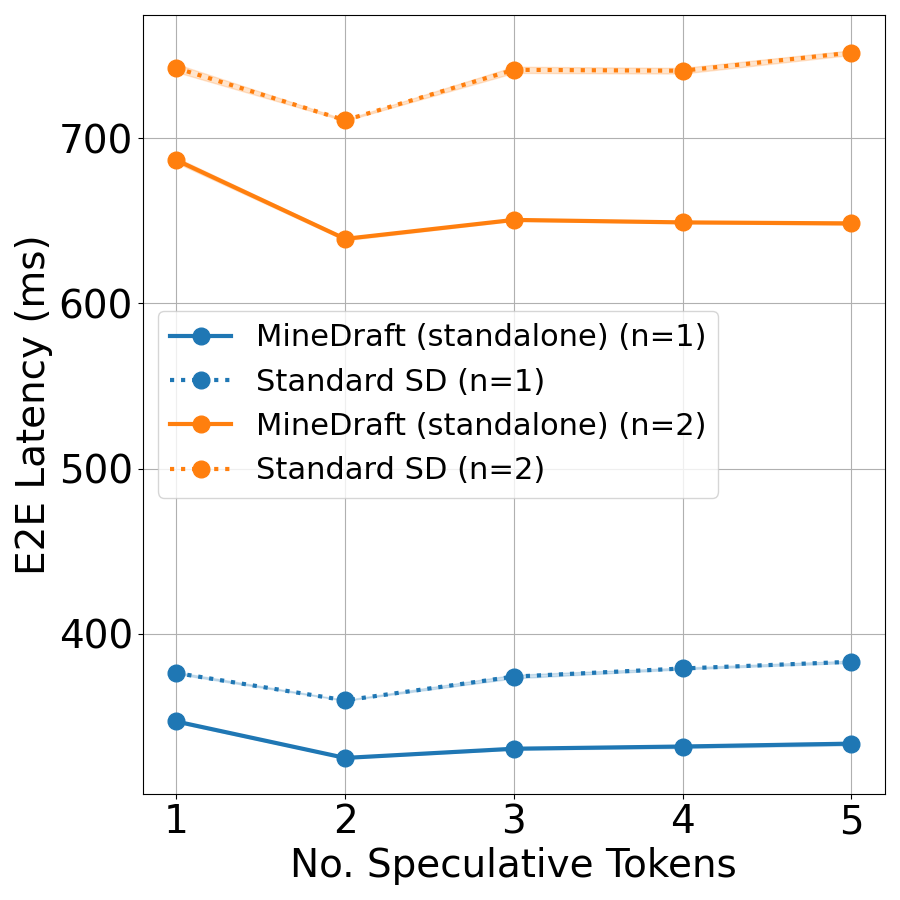
\includegraphics[width=0.23\linewidth]{results/ShareGPT_Meta-Llama-3_3-70B-Instruct-AWQ-INT4_Llama-3_1-8B-Instruct_1000_bs64_100pct_latency_vs_n.png} &
        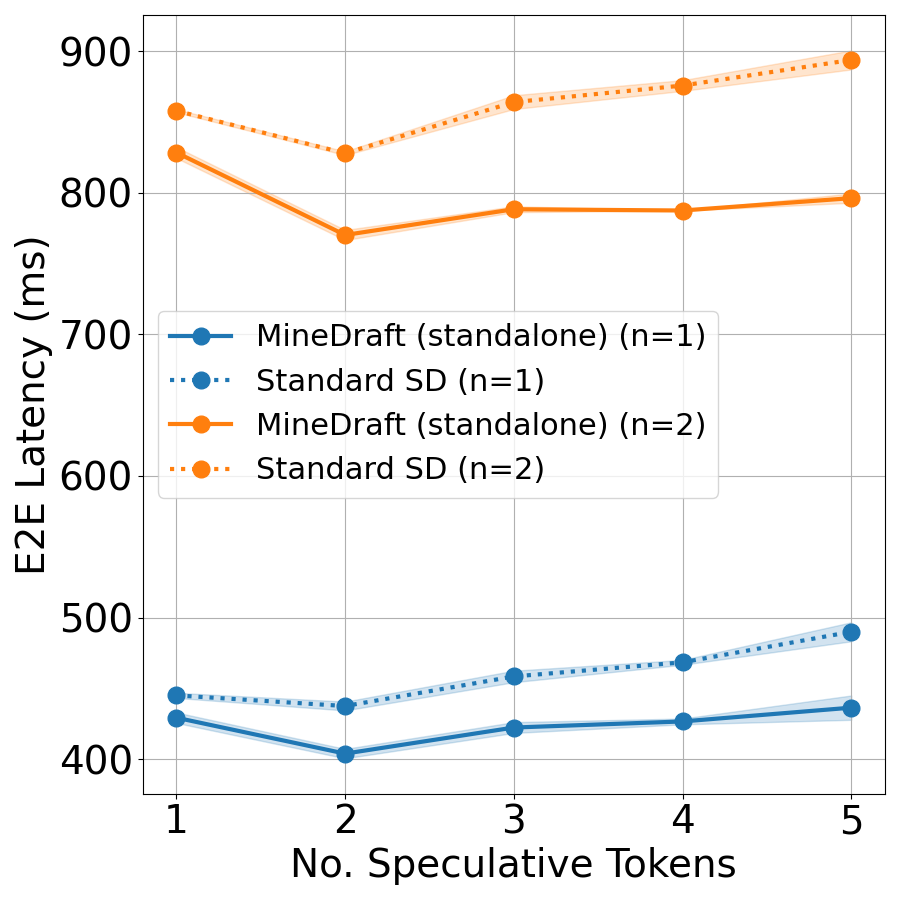
\includegraphics[width=0.23\linewidth]{results/Spec-Bench_Meta-Llama-3_3-70B-Instruct-AWQ-INT4_Llama-3_1-8B-Instruct_160_bs64_100pct_latency_vs_n.png} &
        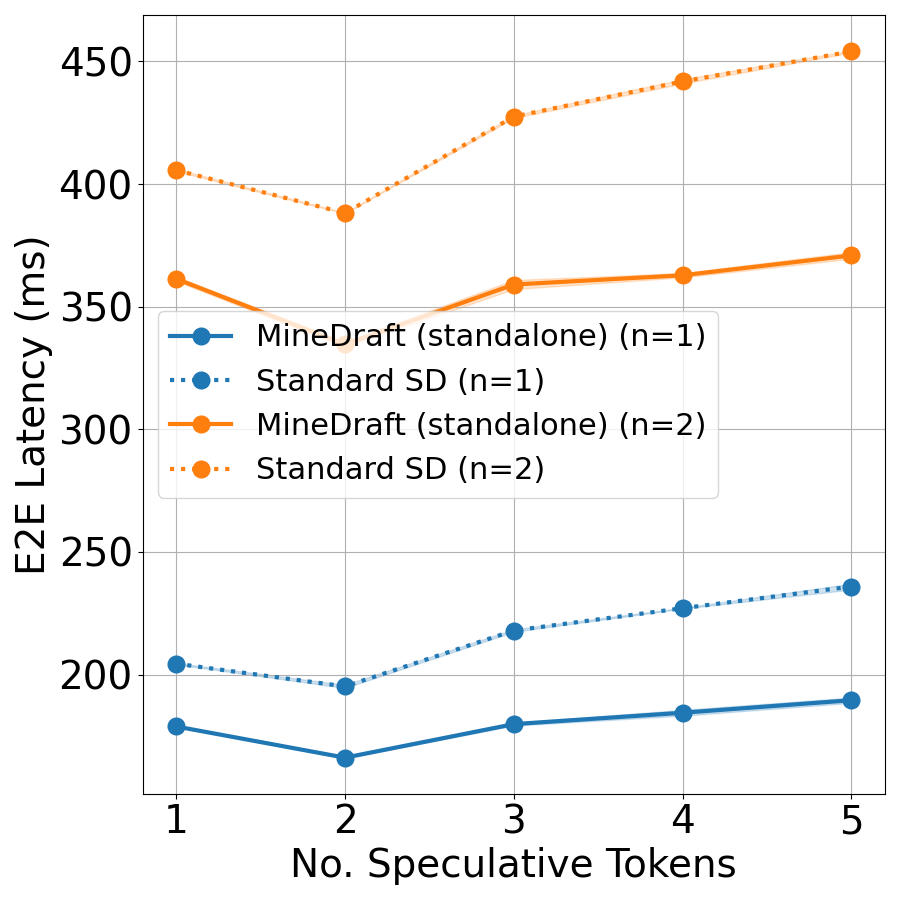
\includegraphics[width=0.23\linewidth]{results/Tough_Meta-Llama-3_3-70B-Instruct-AWQ-INT4_Llama-3_1-8B-Instruct_1000_bs64_100pct_latency_vs_n.png} \\

    \end{tabular}}
    \caption{End-to-End Latency (ms) comparison against standard SD across various $n$ on model setting 5.
    }
    \label{fig:e2elatencty-n-llama}
\end{figure*}


\begin{figure*}[!ht]
    \centering
    \setlength{\tabcolsep}{1pt} 
    \resizebox{0.99\linewidth}{!}{
    \begin{tabular}{ccccc}
        & \hspace{8mm}\textbf{Arena} & \hspace{8mm}\textbf{ShareGPT} & \hspace{8mm}\textbf{Spec-Bench}  & \hspace{8mm}\textbf{Tough}\\

        \rotatebox{90}{\parbox{3.5cm}{\centering \hspace{10mm}\textbf{Qwen3~32B-0.6B}}} &
        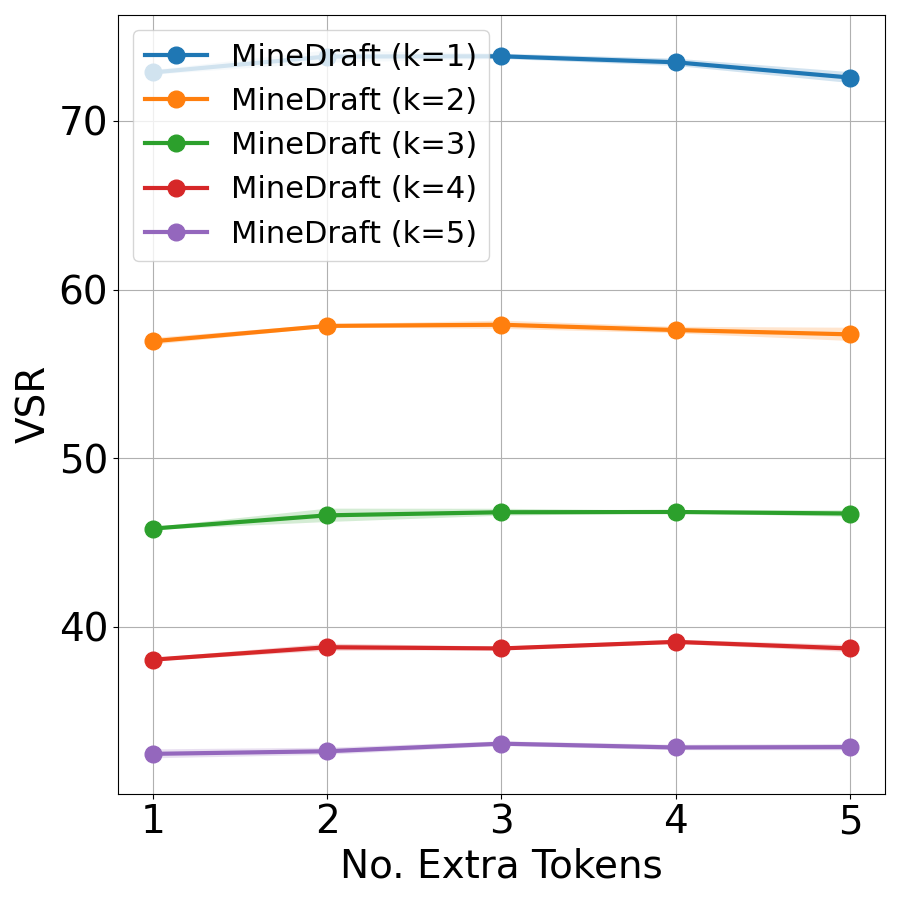
\includegraphics[width=0.23\linewidth]{results/Arena_Qwen3-32B_Qwen3-0_6B_1000_bs16_100pct_vsr_vs_e.png} &
        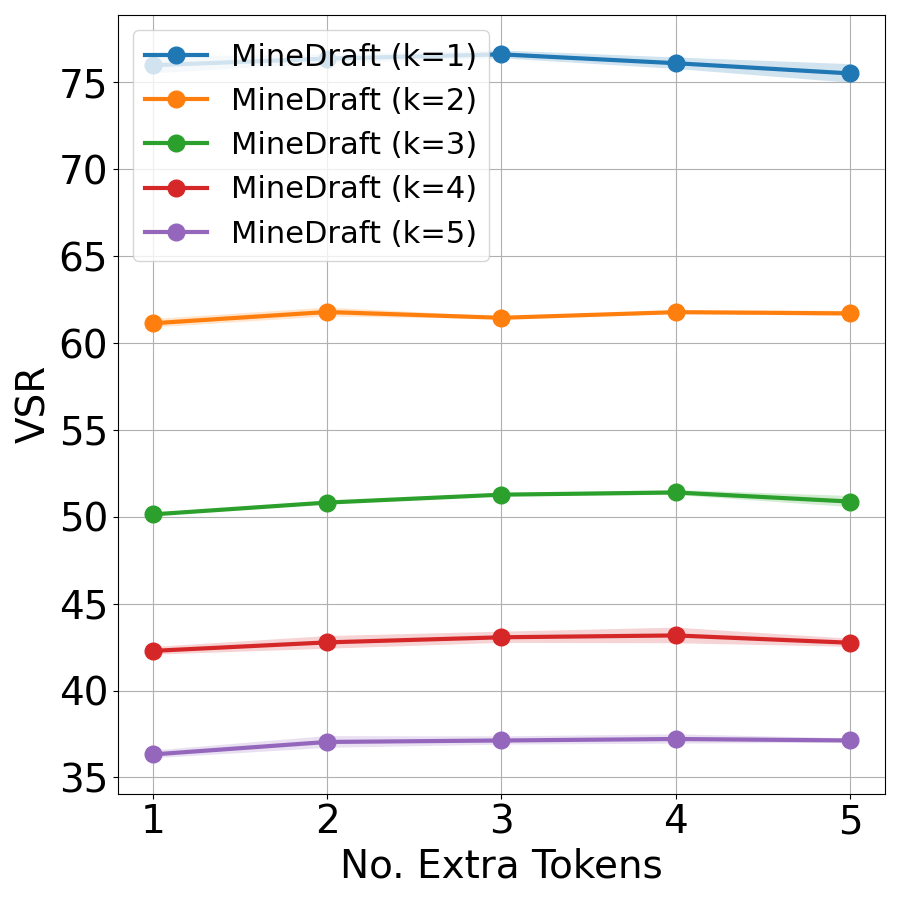
\includegraphics[width=0.23\linewidth]{results/ShareGPT_Qwen3-32B_Qwen3-0_6B_1000_bs16_100pct_vsr_vs_e.png} &
        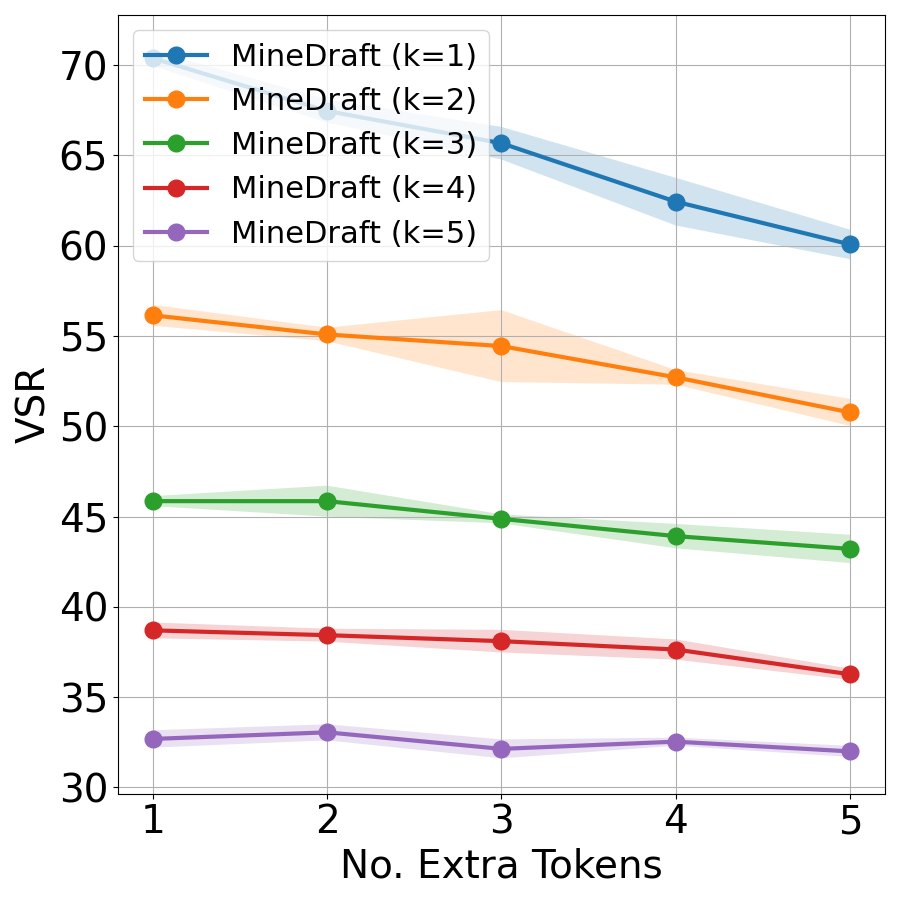
\includegraphics[width=0.23\linewidth]{results/Spec-Bench_Qwen3-32B_Qwen3-0_6B_161_bs16_100pct_vsr_vs_e.png} &
        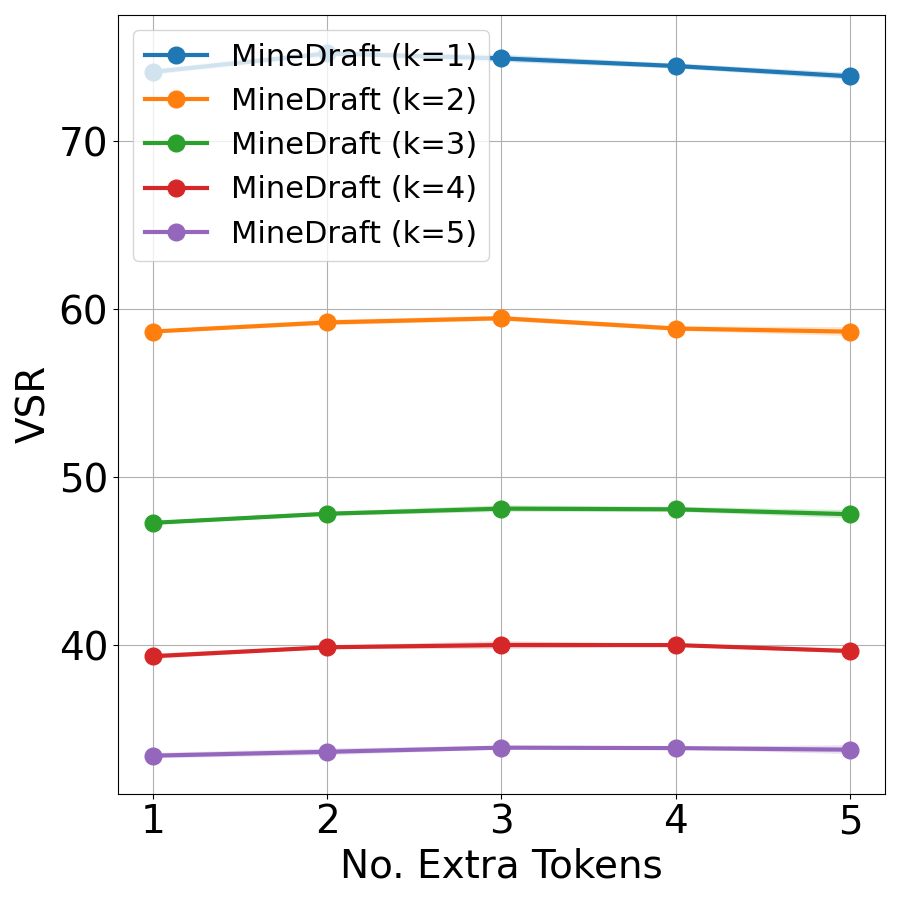
\includegraphics[width=0.23\linewidth]{results/Tough_Qwen3-32B_Qwen3-0_6B_1000_bs16_100pct_vsr_vs_e.png} \\
    \end{tabular}}
    \caption{VSR comparison for \alg{} with TETRIS across extra tokens on model setting 1.    
    }
    \label{fig:vsr-vs-e-all}
\end{figure*}


\begin{figure*}[!ht]
    \centering
    \setlength{\tabcolsep}{1pt} 
    \resizebox{0.99\linewidth}{!}{
    \begin{tabular}{ccccc}
        & \hspace{8mm}\textbf{Arena} & \hspace{8mm}\textbf{ShareGPT} & \hspace{8mm}\textbf{Spec-Bench}  & \hspace{8mm}\textbf{Tough}\\

        \rotatebox{90}{\parbox{3.5cm}{\centering \hspace{10mm}\textbf{$e = 1$}}} &
        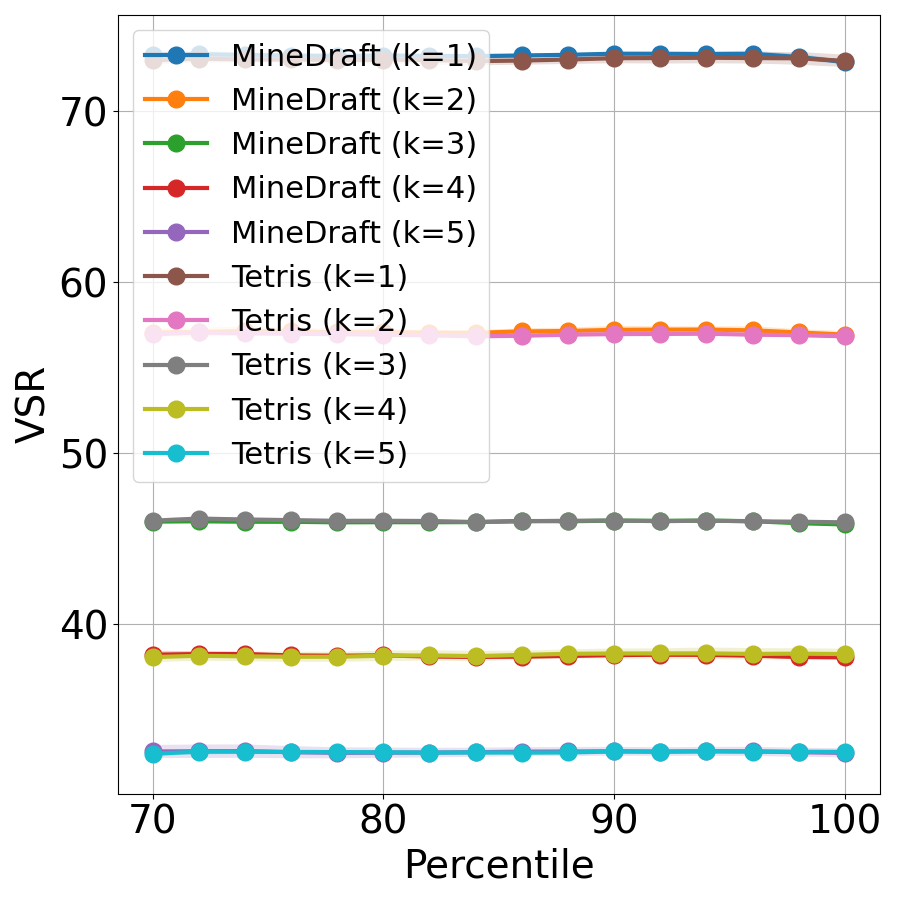
\includegraphics[width=0.23\linewidth]{results/Arena_Qwen3-32B_Qwen3-0_6B_1000_bs16_n1_e1_vsr_vs_percentage.png} &
        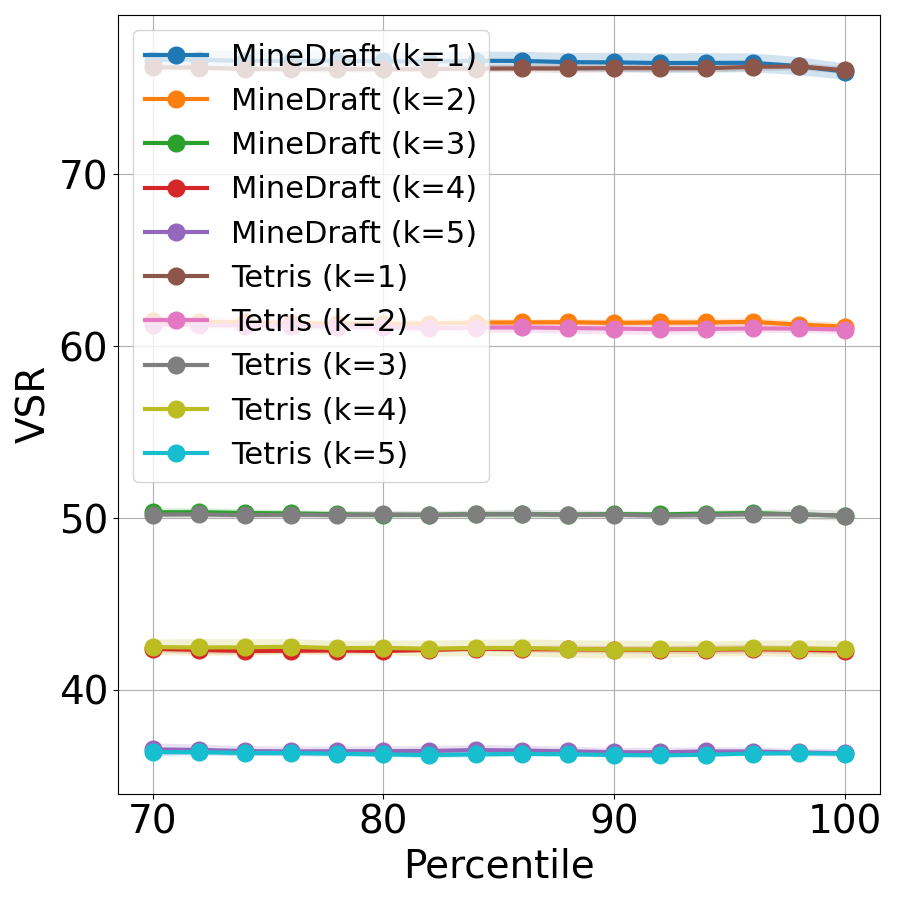
\includegraphics[width=0.23\linewidth]{results/ShareGPT_Qwen3-32B_Qwen3-0_6B_1000_bs16_n1_e1_vsr_vs_percentage.png} &
        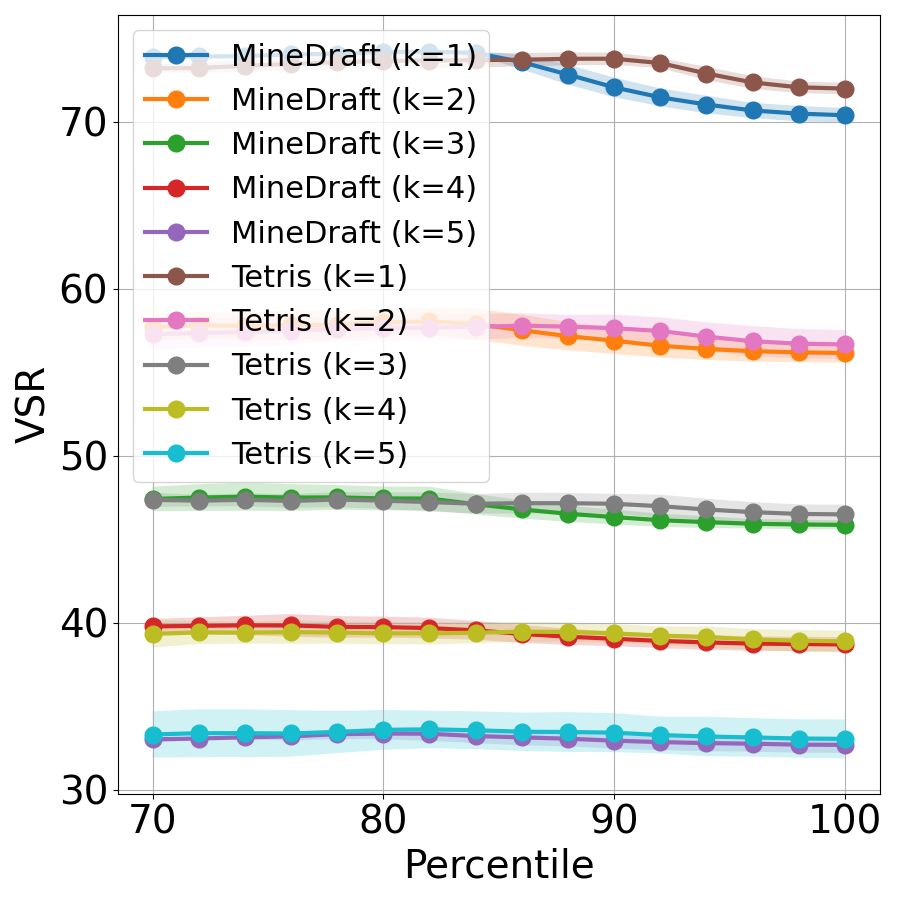
\includegraphics[width=0.23\linewidth]{results/Spec-Bench_Qwen3-32B_Qwen3-0_6B_161_bs16_n1_e1_vsr_vs_percentage.png} &
        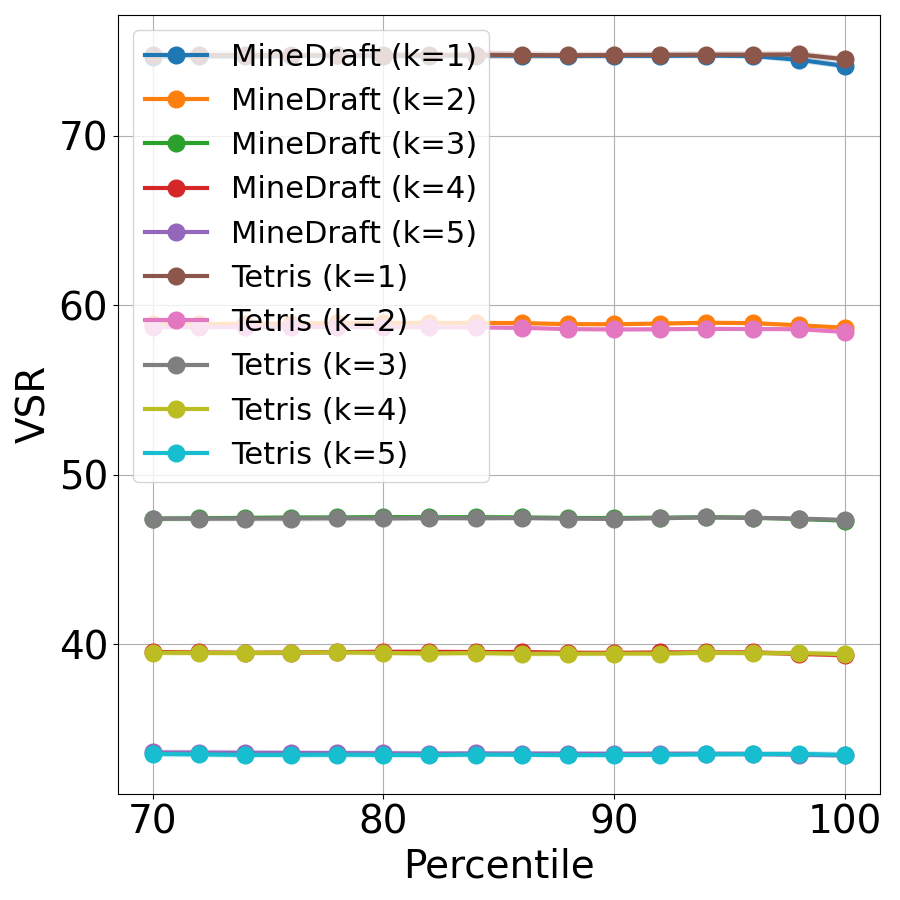
\includegraphics[width=0.23\linewidth]{results/Tough_Qwen3-32B_Qwen3-0_6B_1000_bs16_n1_e1_vsr_vs_percentage.png} \\

        \rotatebox{90}{\parbox{3.5cm}{\centering \hspace{10mm}\textbf{$e = 2$}}} &
        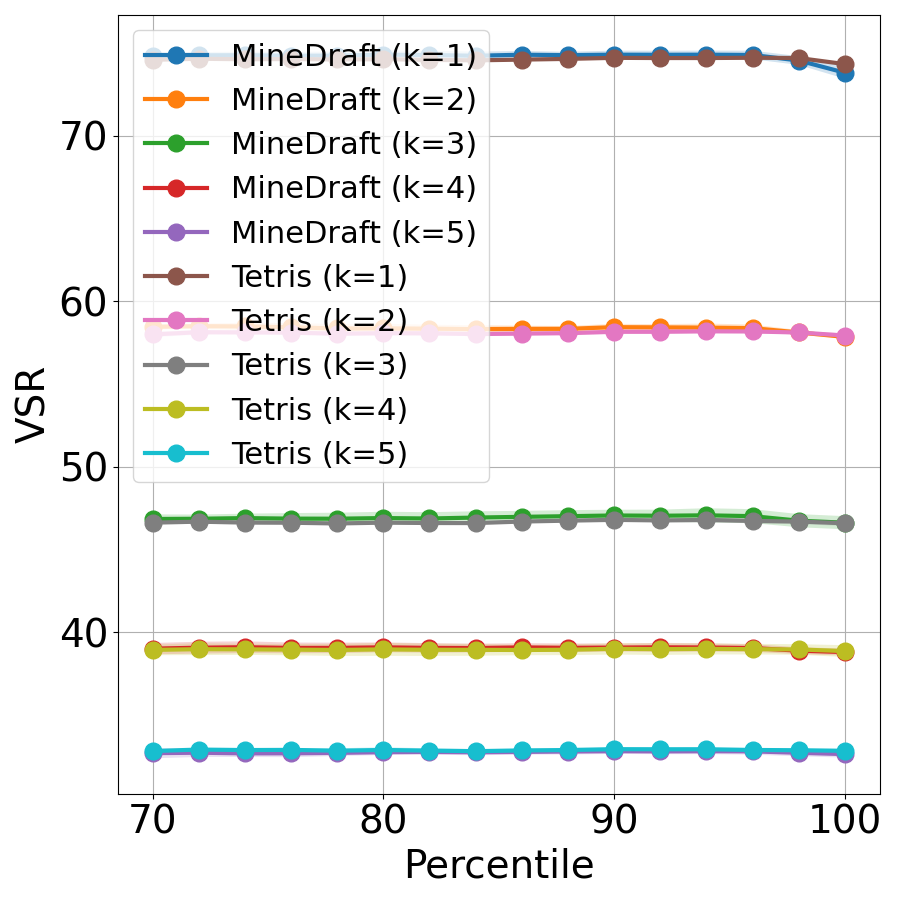
\includegraphics[width=0.23\linewidth]{results/Arena_Qwen3-32B_Qwen3-0_6B_1000_bs16_n1_e2_vsr_vs_percentage.png} &
        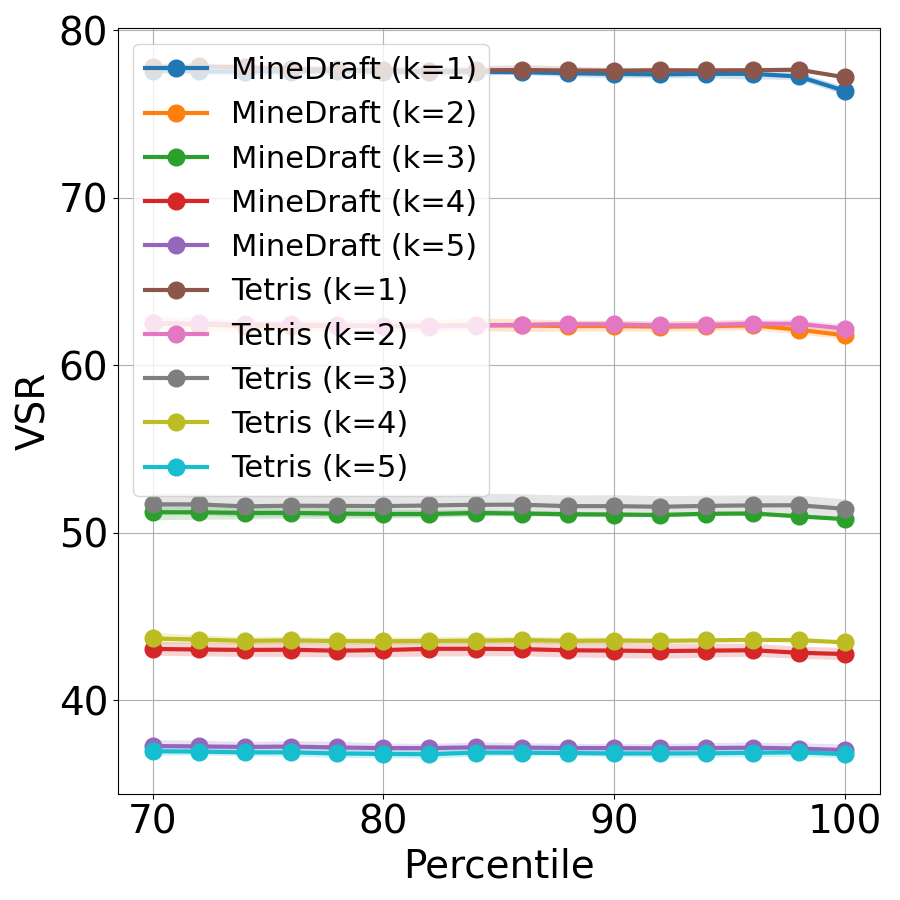
\includegraphics[width=0.23\linewidth]{results/ShareGPT_Qwen3-32B_Qwen3-0_6B_1000_bs16_n1_e2_vsr_vs_percentage.png} &
        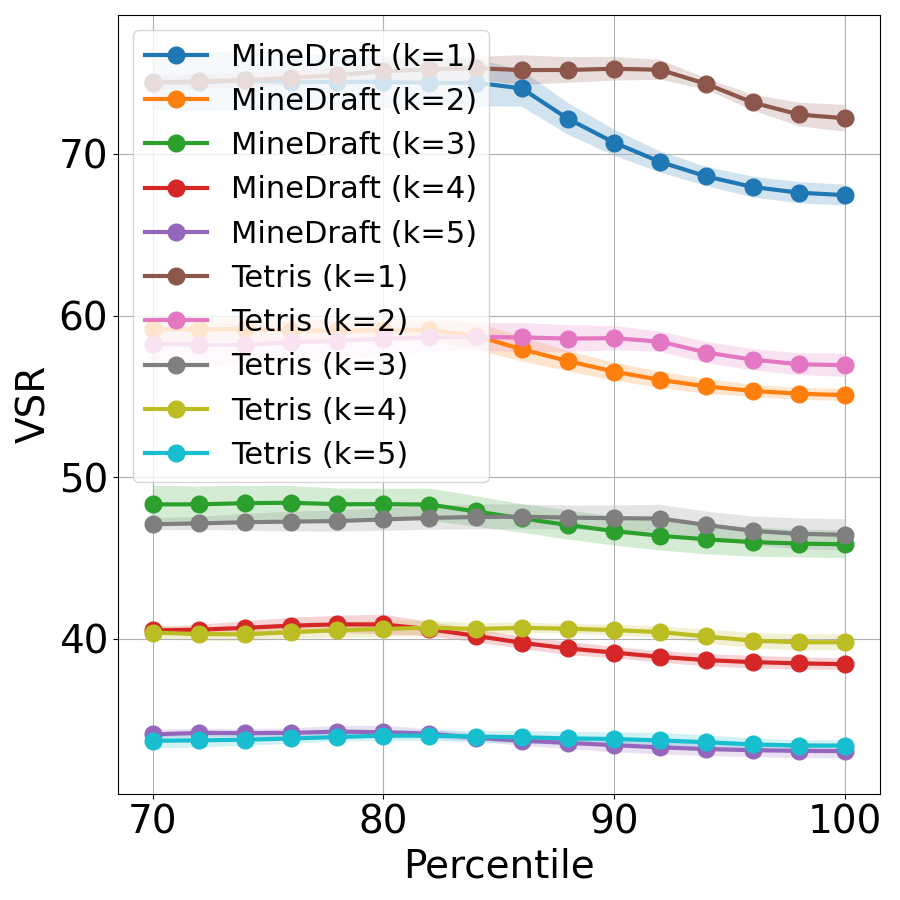
\includegraphics[width=0.23\linewidth]{results/Spec-Bench_Qwen3-32B_Qwen3-0_6B_161_bs16_n1_e2_vsr_vs_percentage.png} &
        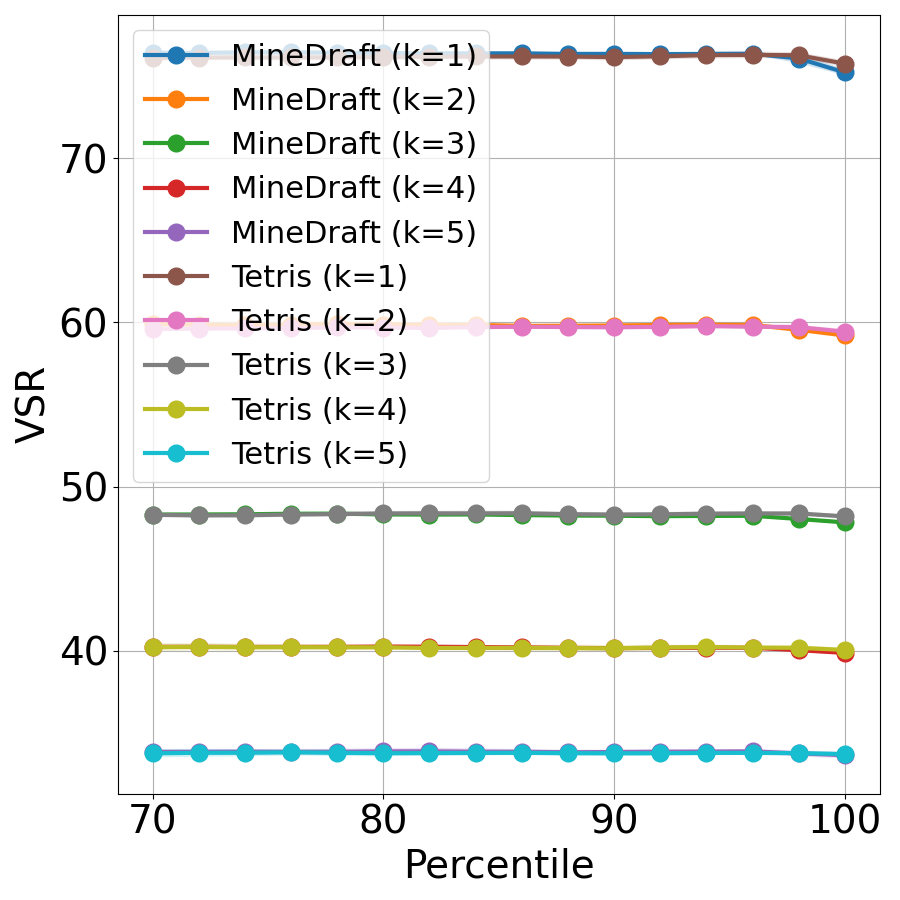
\includegraphics[width=0.23\linewidth]{results/Tough_Qwen3-32B_Qwen3-0_6B_1000_bs16_n1_e2_vsr_vs_percentage.png} \\

        \rotatebox{90}{\parbox{3.5cm}{\centering \hspace{10mm}\textbf{$e = 3$}}} &
        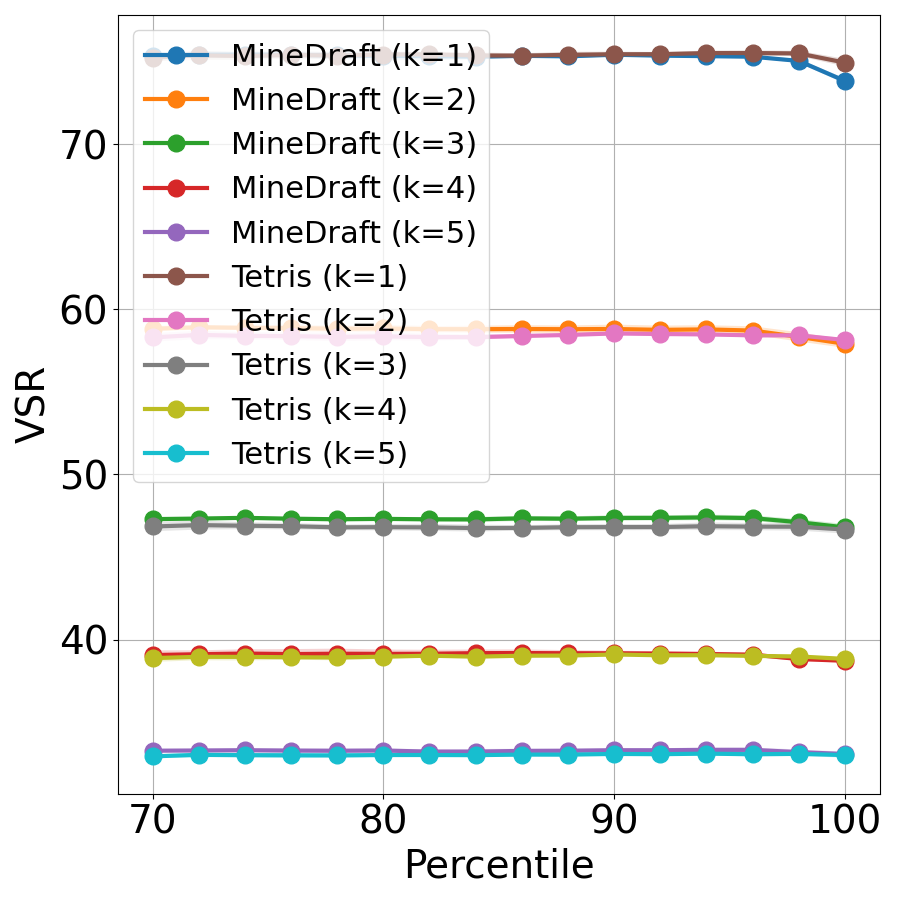
\includegraphics[width=0.23\linewidth]{results/Arena_Qwen3-32B_Qwen3-0_6B_1000_bs16_n1_e3_vsr_vs_percentage.png} &
        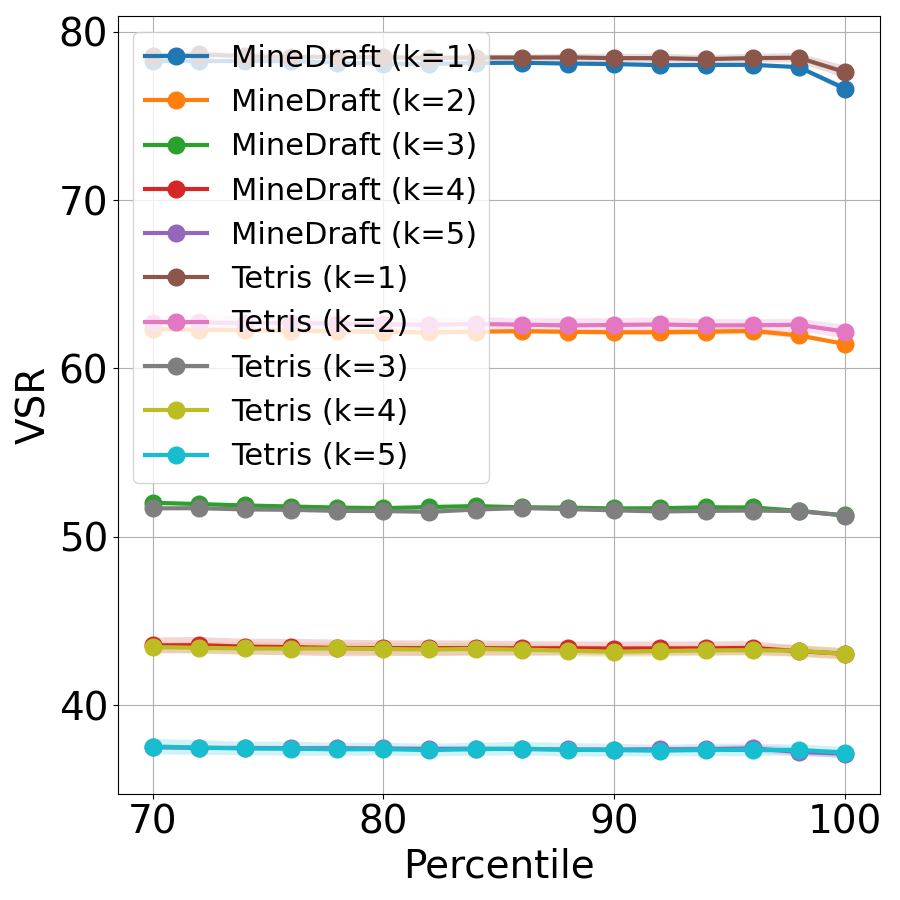
\includegraphics[width=0.23\linewidth]{results/ShareGPT_Qwen3-32B_Qwen3-0_6B_1000_bs16_n1_e3_vsr_vs_percentage.png} &
        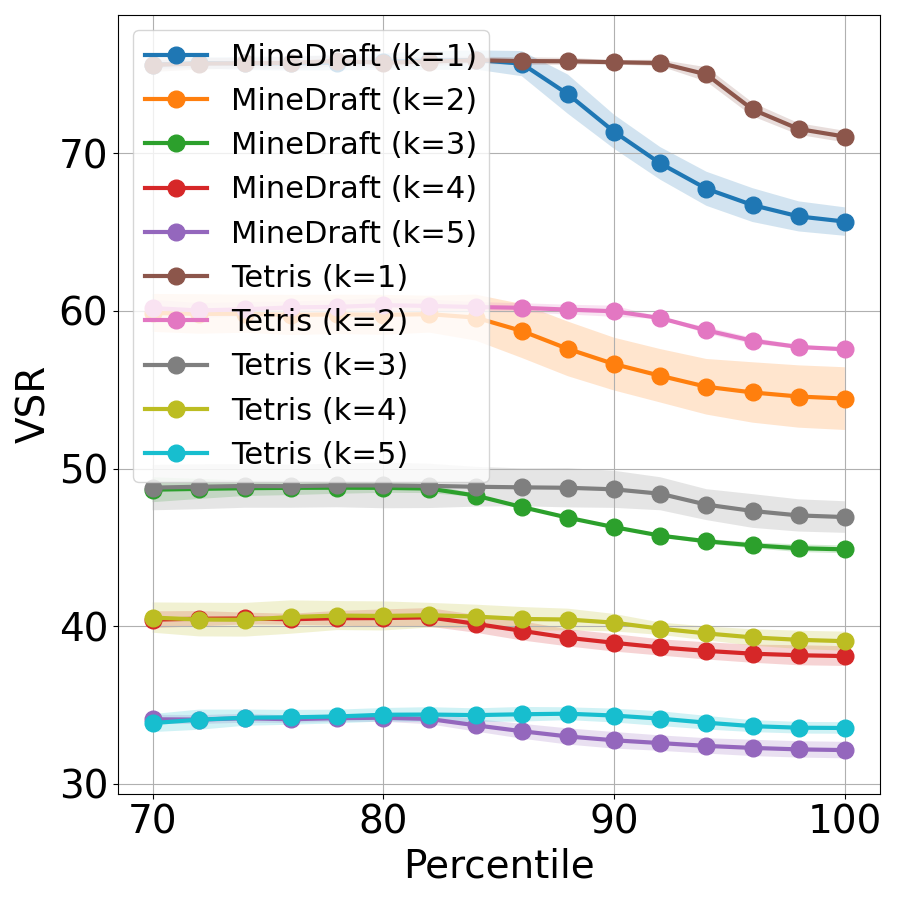
\includegraphics[width=0.23\linewidth]{results/Spec-Bench_Qwen3-32B_Qwen3-0_6B_161_bs16_n1_e3_vsr_vs_percentage.png} &
        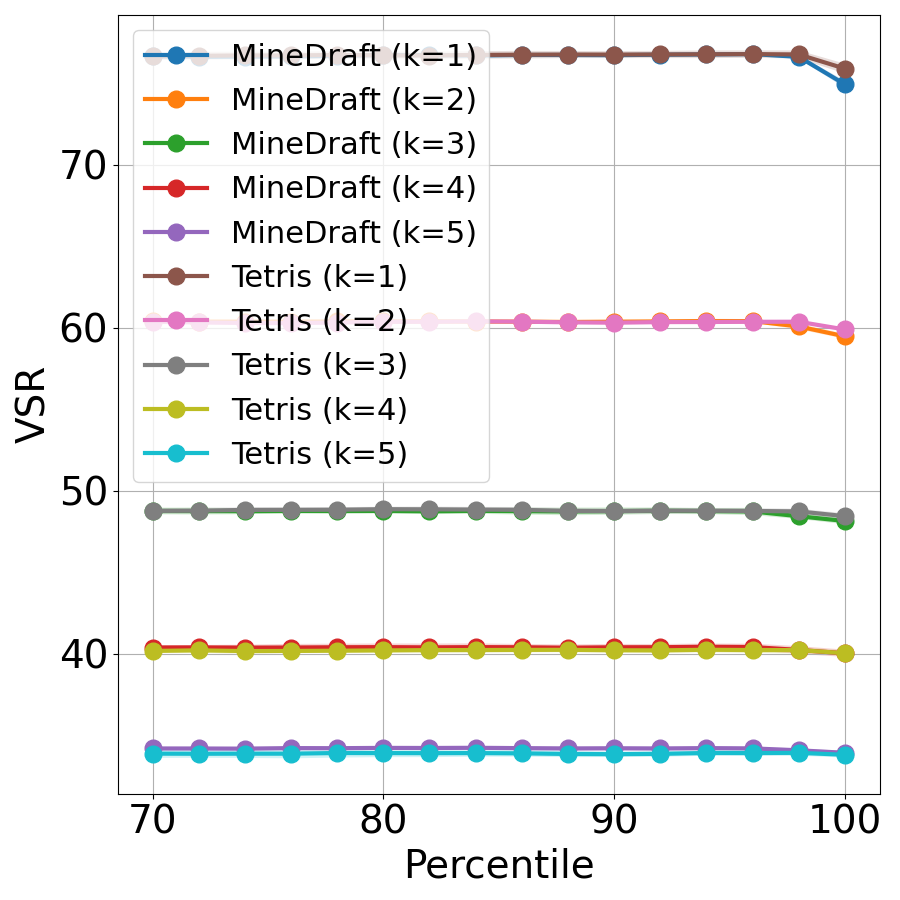
\includegraphics[width=0.23\linewidth]{results/Tough_Qwen3-32B_Qwen3-0_6B_1000_bs16_n1_e3_vsr_vs_percentage.png} \\

        \rotatebox{90}{\parbox{3.5cm}{\centering \hspace{10mm}\textbf{$e = 4$}}} &
        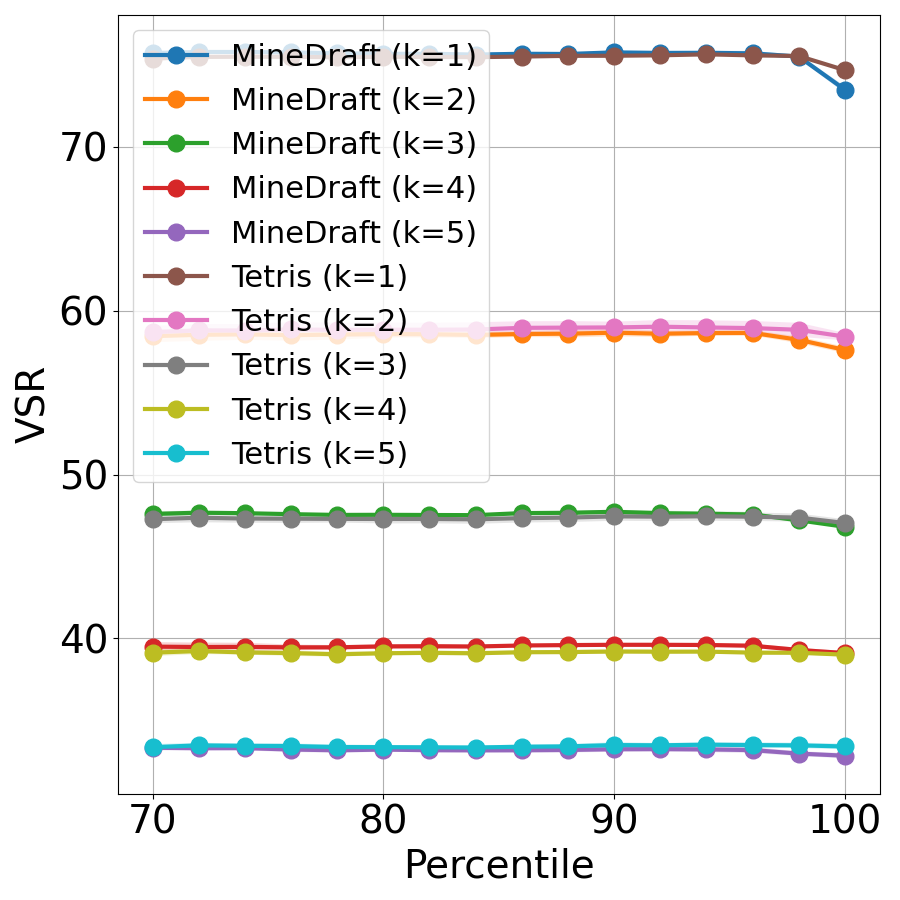
\includegraphics[width=0.23\linewidth]{results/Arena_Qwen3-32B_Qwen3-0_6B_1000_bs16_n1_e4_vsr_vs_percentage.png} &
        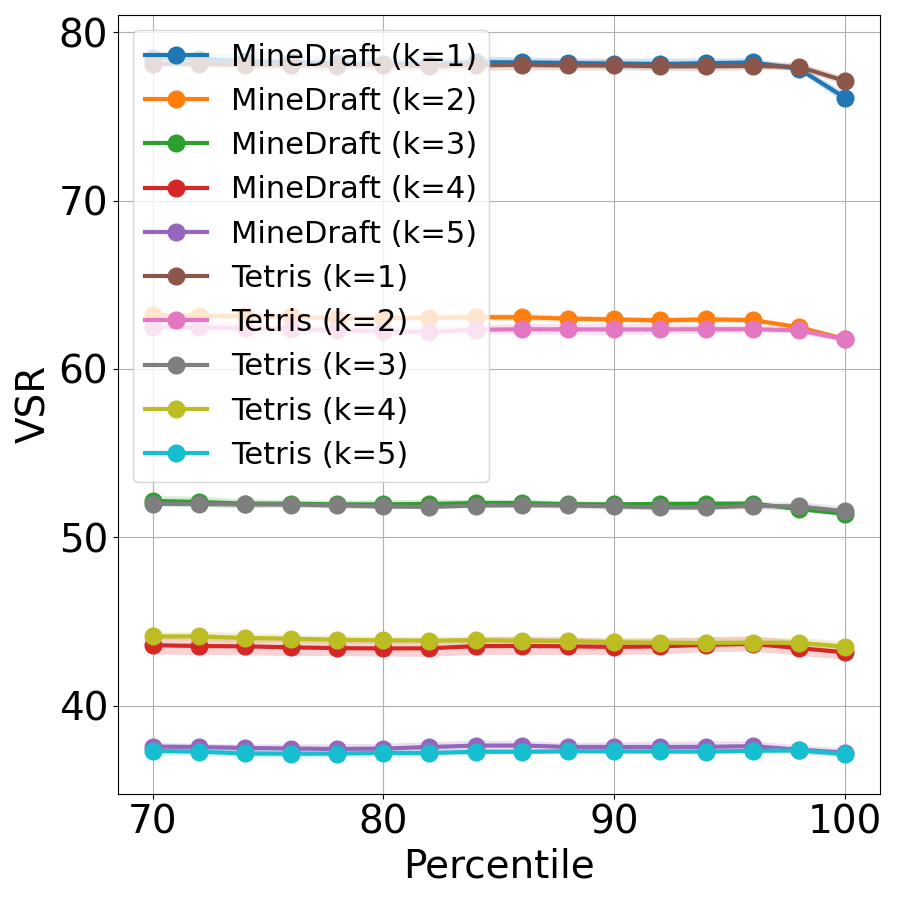
\includegraphics[width=0.23\linewidth]{results/ShareGPT_Qwen3-32B_Qwen3-0_6B_1000_bs16_n1_e4_vsr_vs_percentage.png} &
        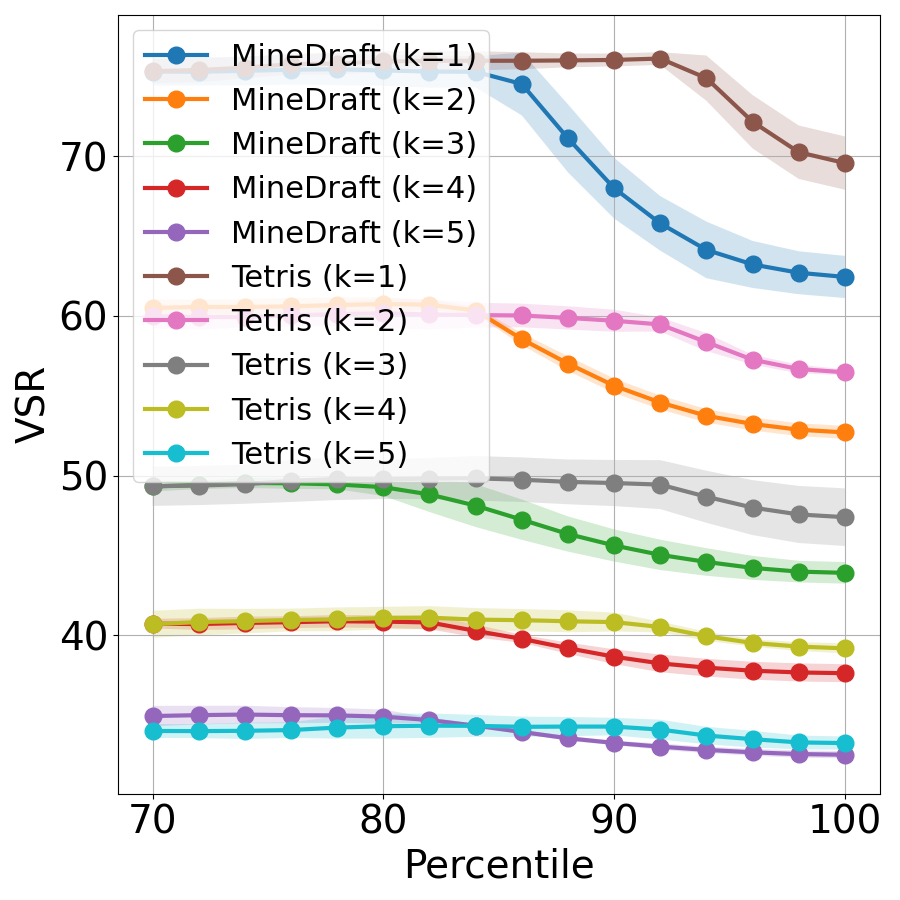
\includegraphics[width=0.23\linewidth]{results/Spec-Bench_Qwen3-32B_Qwen3-0_6B_161_bs16_n1_e4_vsr_vs_percentage.png} &
        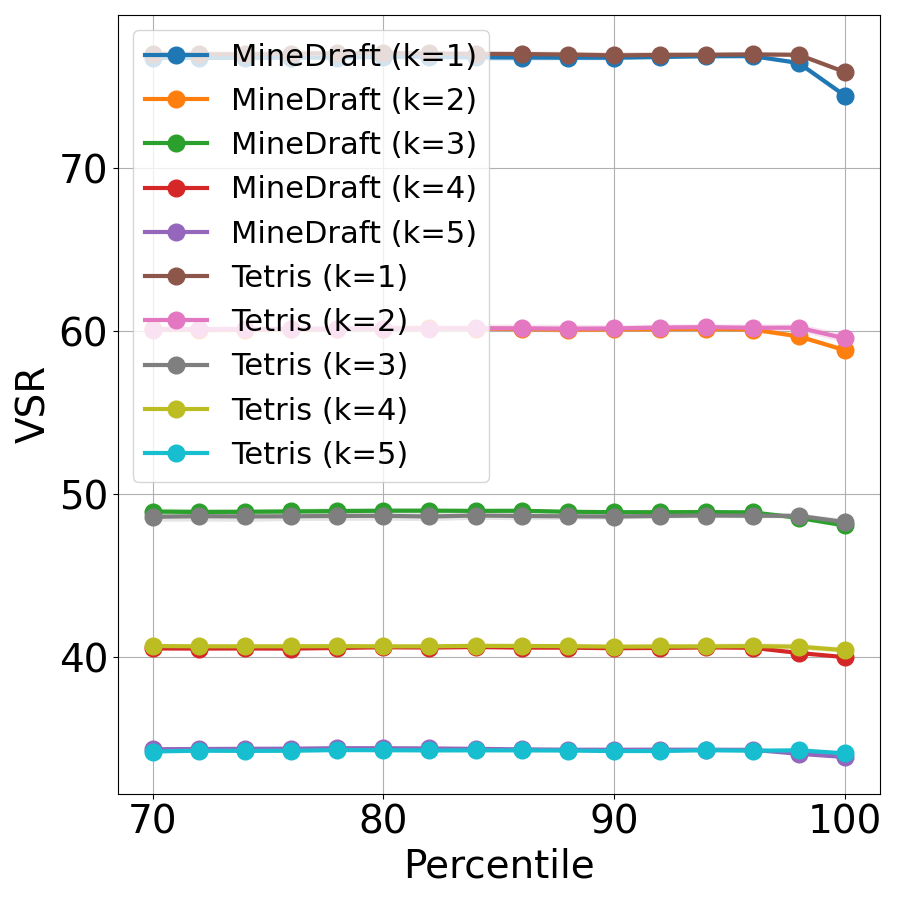
\includegraphics[width=0.23\linewidth]{results/Tough_Qwen3-32B_Qwen3-0_6B_1000_bs16_n1_e4_vsr_vs_percentage.png} \\

        \rotatebox{90}{\parbox{3.5cm}{\centering \hspace{10mm}\textbf{$e = 5$}}} &
        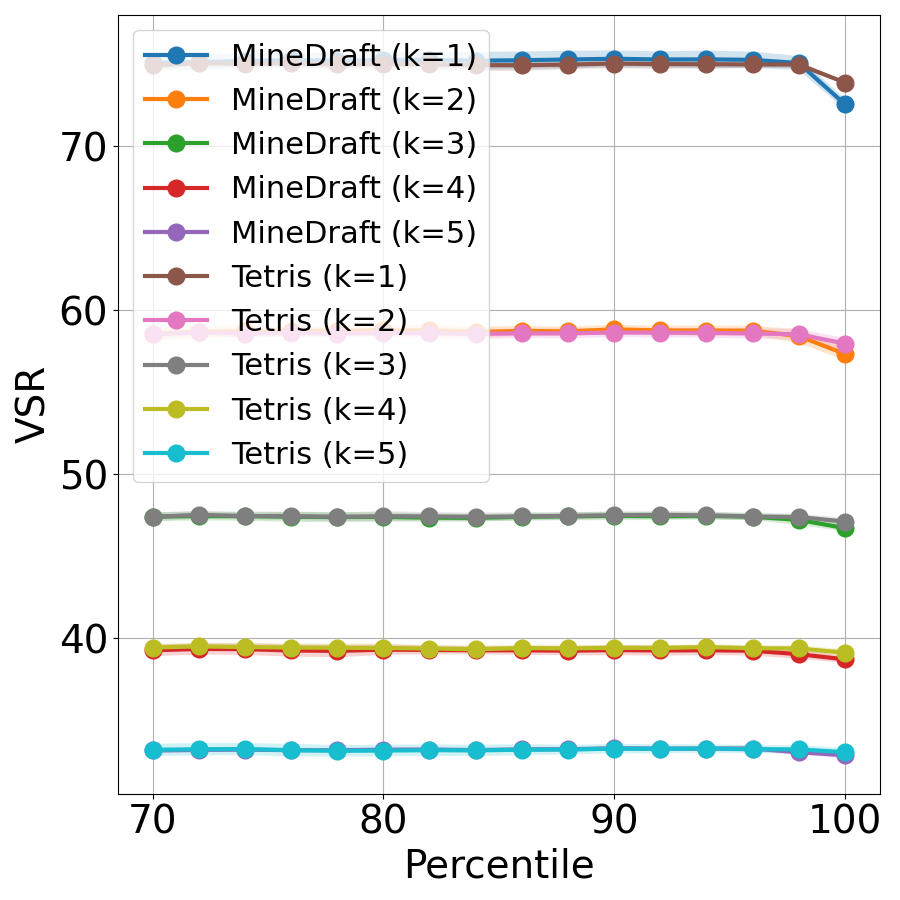
\includegraphics[width=0.23\linewidth]{results/Arena_Qwen3-32B_Qwen3-0_6B_1000_bs16_n1_e5_vsr_vs_percentage.png} &
        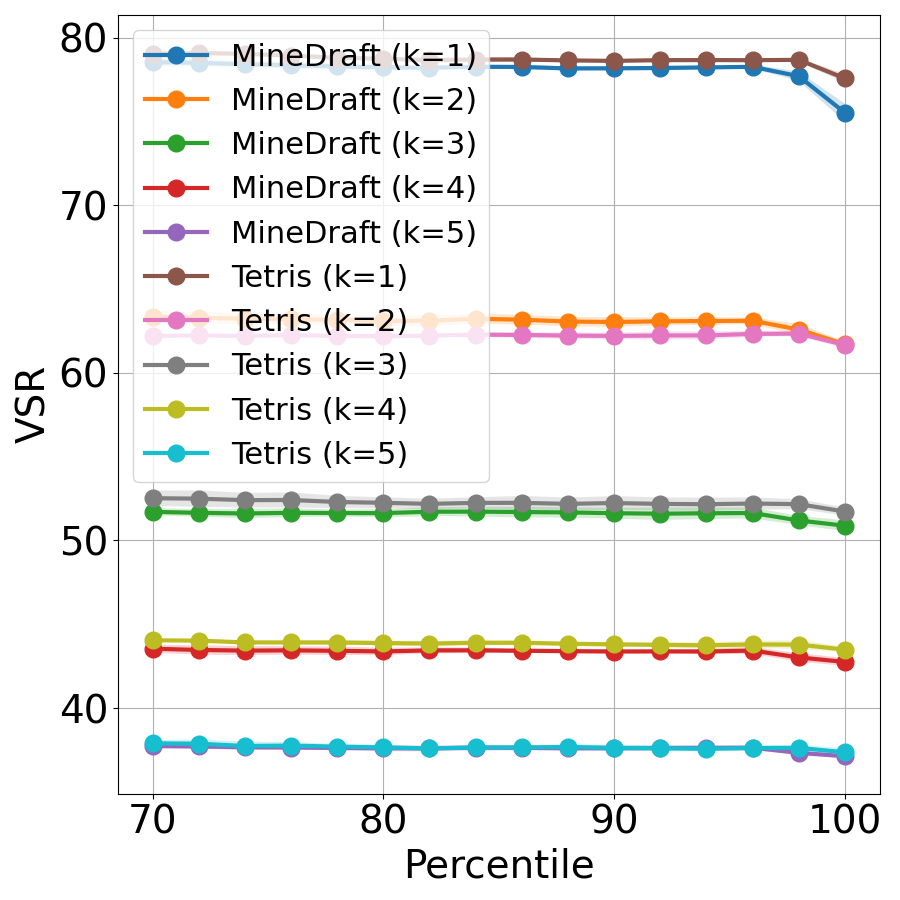
\includegraphics[width=0.23\linewidth]{results/ShareGPT_Qwen3-32B_Qwen3-0_6B_1000_bs16_n1_e5_vsr_vs_percentage.png} &
        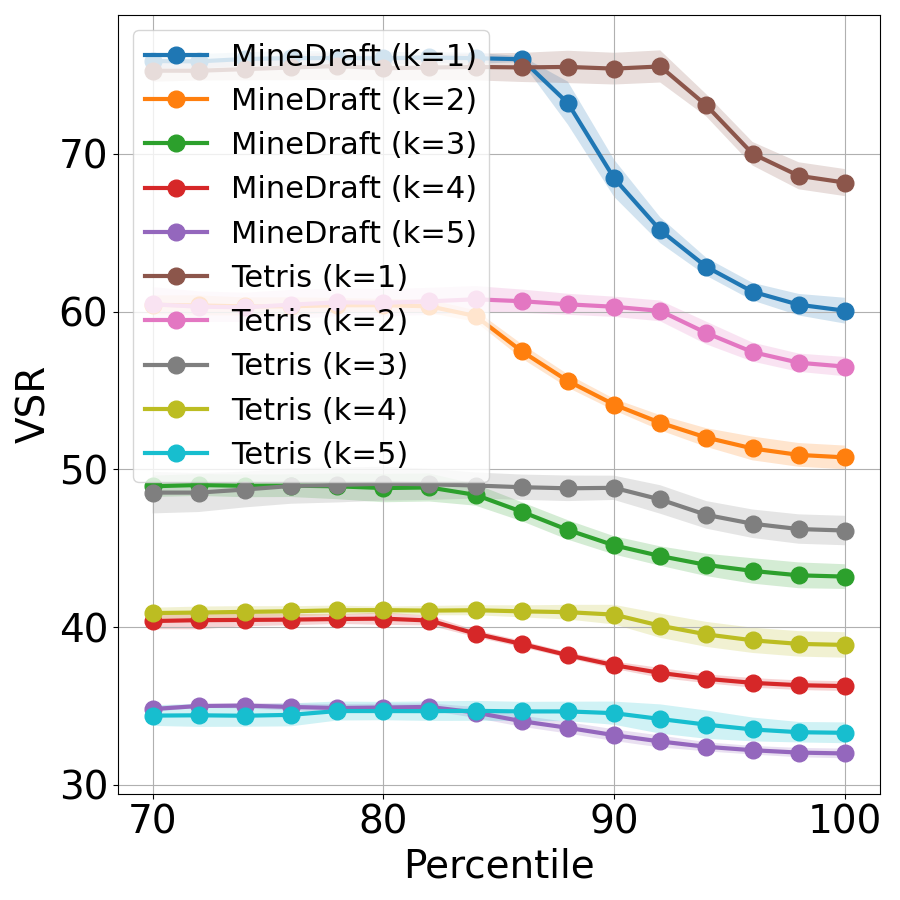
\includegraphics[width=0.23\linewidth]{results/Spec-Bench_Qwen3-32B_Qwen3-0_6B_161_bs16_n1_e5_vsr_vs_percentage.png} &
        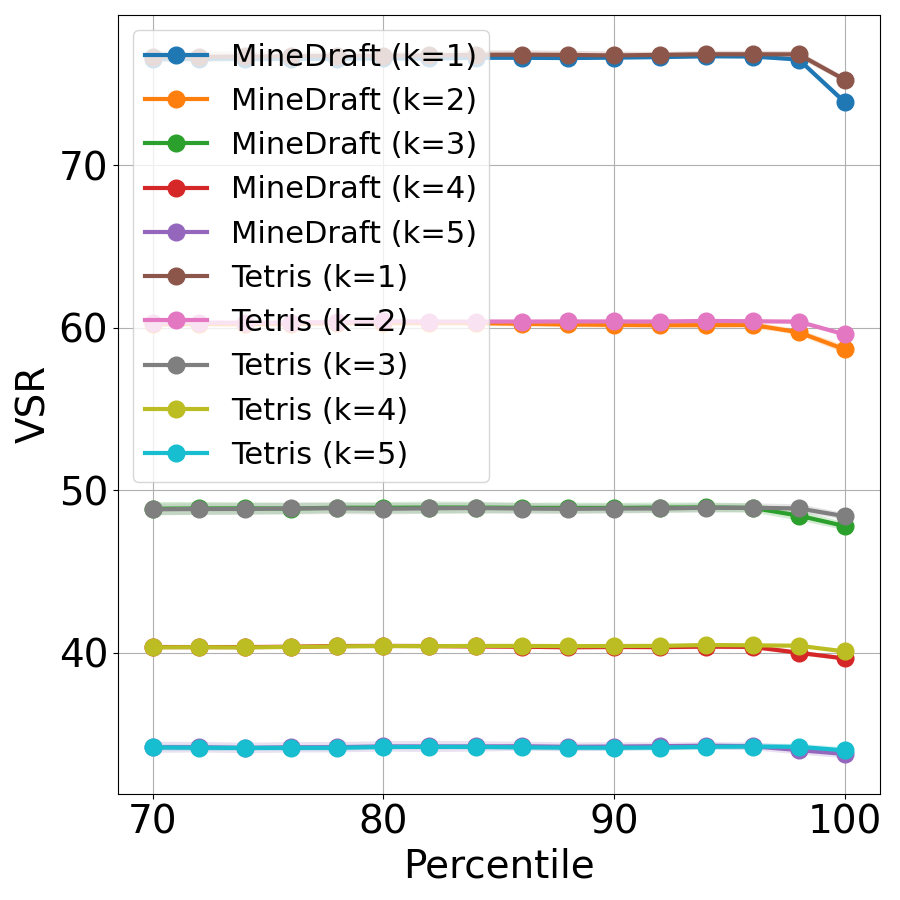
\includegraphics[width=0.23\linewidth]{results/Tough_Qwen3-32B_Qwen3-0_6B_1000_bs16_n1_e5_vsr_vs_percentage.png} \\
    \end{tabular}}
    \caption{VSR comparison for \alg{} with TETRIS and standalone TETRIS across trimming percentiles on model setting 1.    
    }
    \label{fig:vsr-vs-percentile-all}
\end{figure*}


\begin{figure*}[!ht]
    \centering
    \setlength{\tabcolsep}{1pt} 
    \resizebox{0.99\linewidth}{!}{
    \begin{tabular}{ccccc}
        & \hspace{8mm}\textbf{Arena} & \hspace{8mm}\textbf{ShareGPT} & \hspace{8mm}\textbf{Spec-Bench}  & \hspace{8mm}\textbf{Tough}\\

        \rotatebox{90}{\parbox{3.5cm}{\centering \hspace{10mm}\textbf{Qwen3~32B-0.6B}}} &
        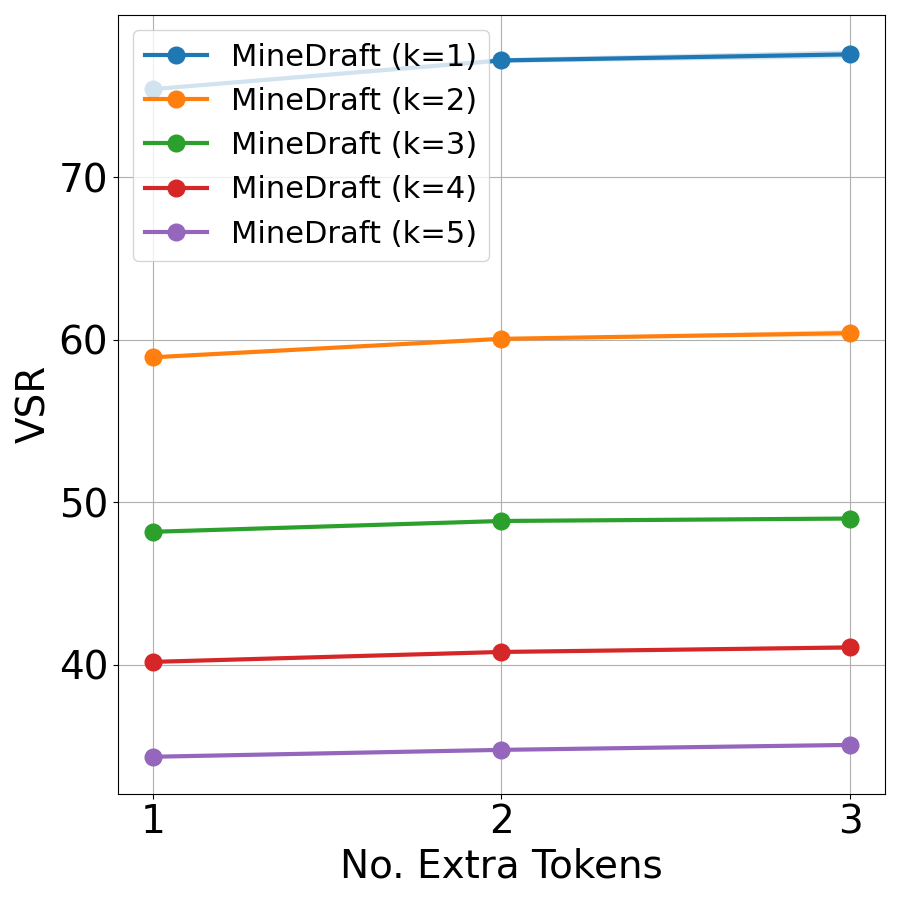
\includegraphics[width=0.23\linewidth]{results/Arena_Qwen3-32B_Qwen3-0_6B_1000_bs16_n2_100pct_vsr_vs_e.png} &
        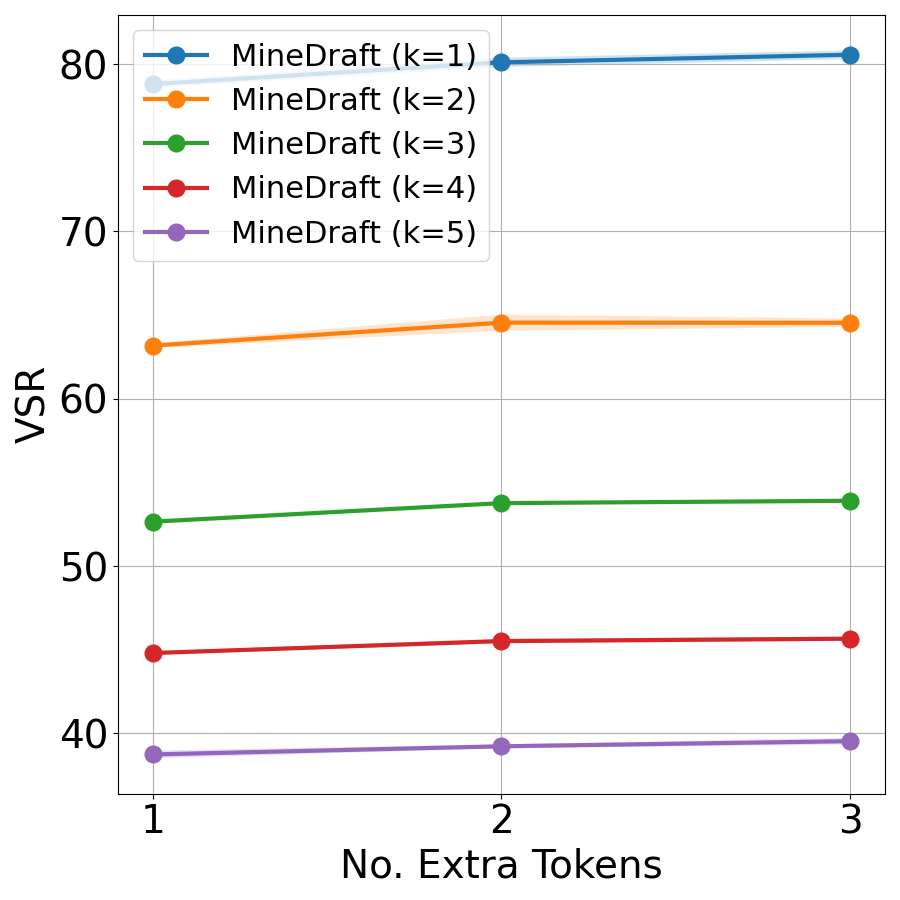
\includegraphics[width=0.23\linewidth]{results/ShareGPT_Qwen3-32B_Qwen3-0_6B_1000_bs16_n2_100pct_vsr_vs_e.png} &
        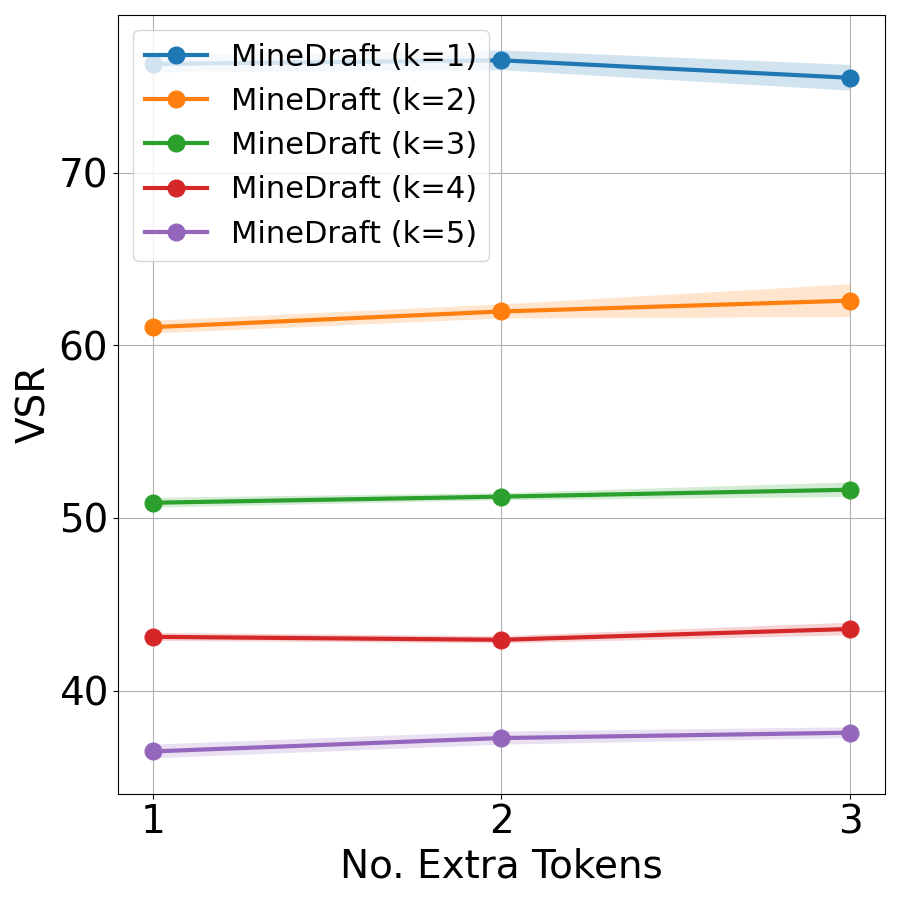
\includegraphics[width=0.23\linewidth]{results/Spec-Bench_Qwen3-32B_Qwen3-0_6B_161_bs16_n2_100pct_vsr_vs_e.png} &
        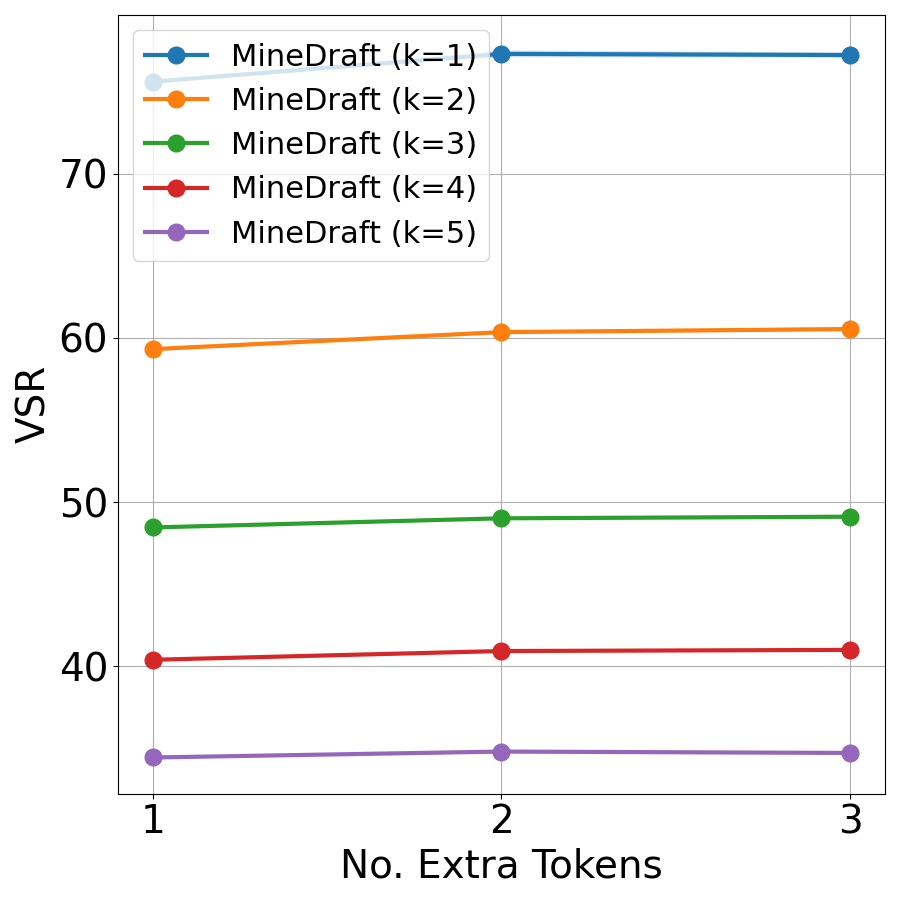
\includegraphics[width=0.23\linewidth]{results/Tough_Qwen3-32B_Qwen3-0_6B_1000_bs16_n2_100pct_vsr_vs_e.png} \\
        
        \rotatebox{90}{\parbox{3.5cm}{\centering \hspace{10mm}\textbf{Llama-3~70B-8B}}} & 
        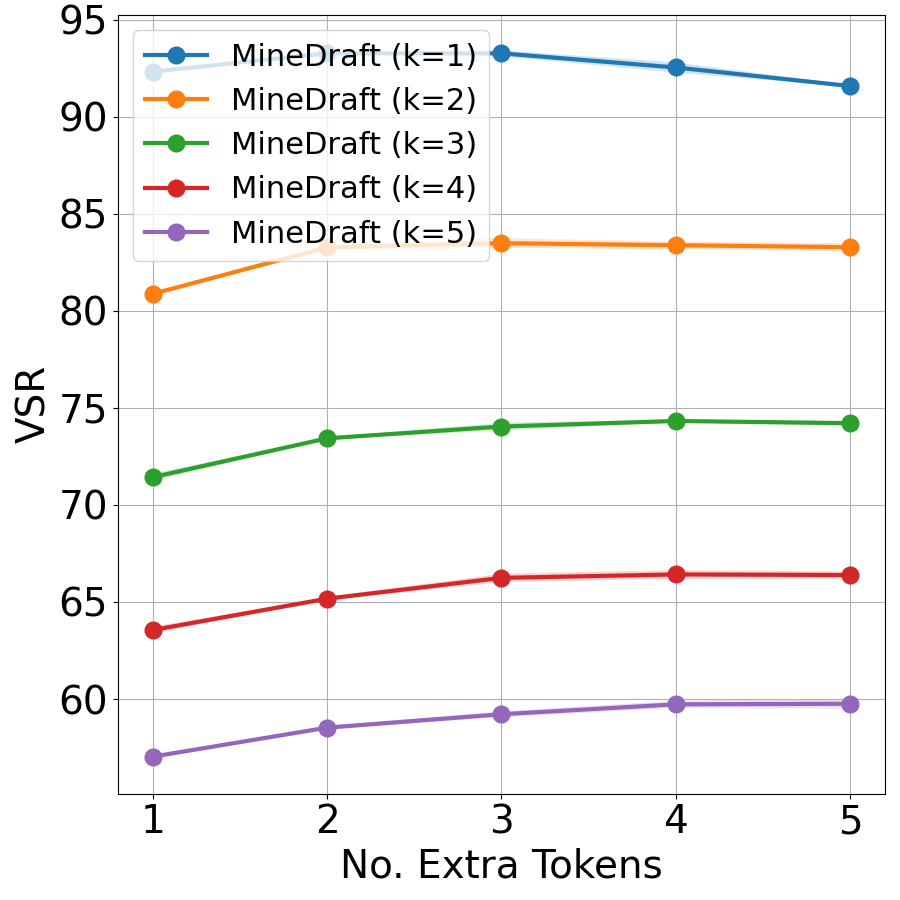
\includegraphics[width=0.23\linewidth]{results/Arena_Meta-Llama-3_3-70B-Instruct-AWQ-INT4_Llama-3_1-8B-Instruct_1000_bs64_n2_100pct_vsr_vs_e.png} &
        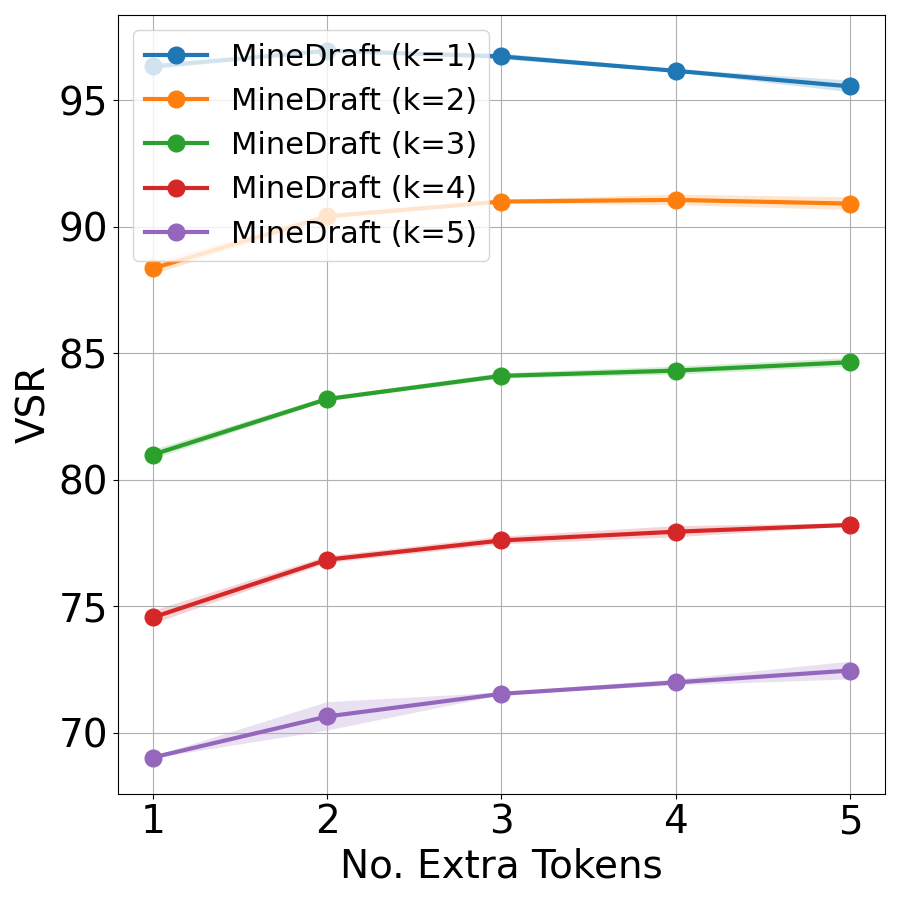
\includegraphics[width=0.23\linewidth]{results/ShareGPT_Meta-Llama-3_3-70B-Instruct-AWQ-INT4_Llama-3_1-8B-Instruct_1000_bs64_n2_100pct_vsr_vs_e.png} &
        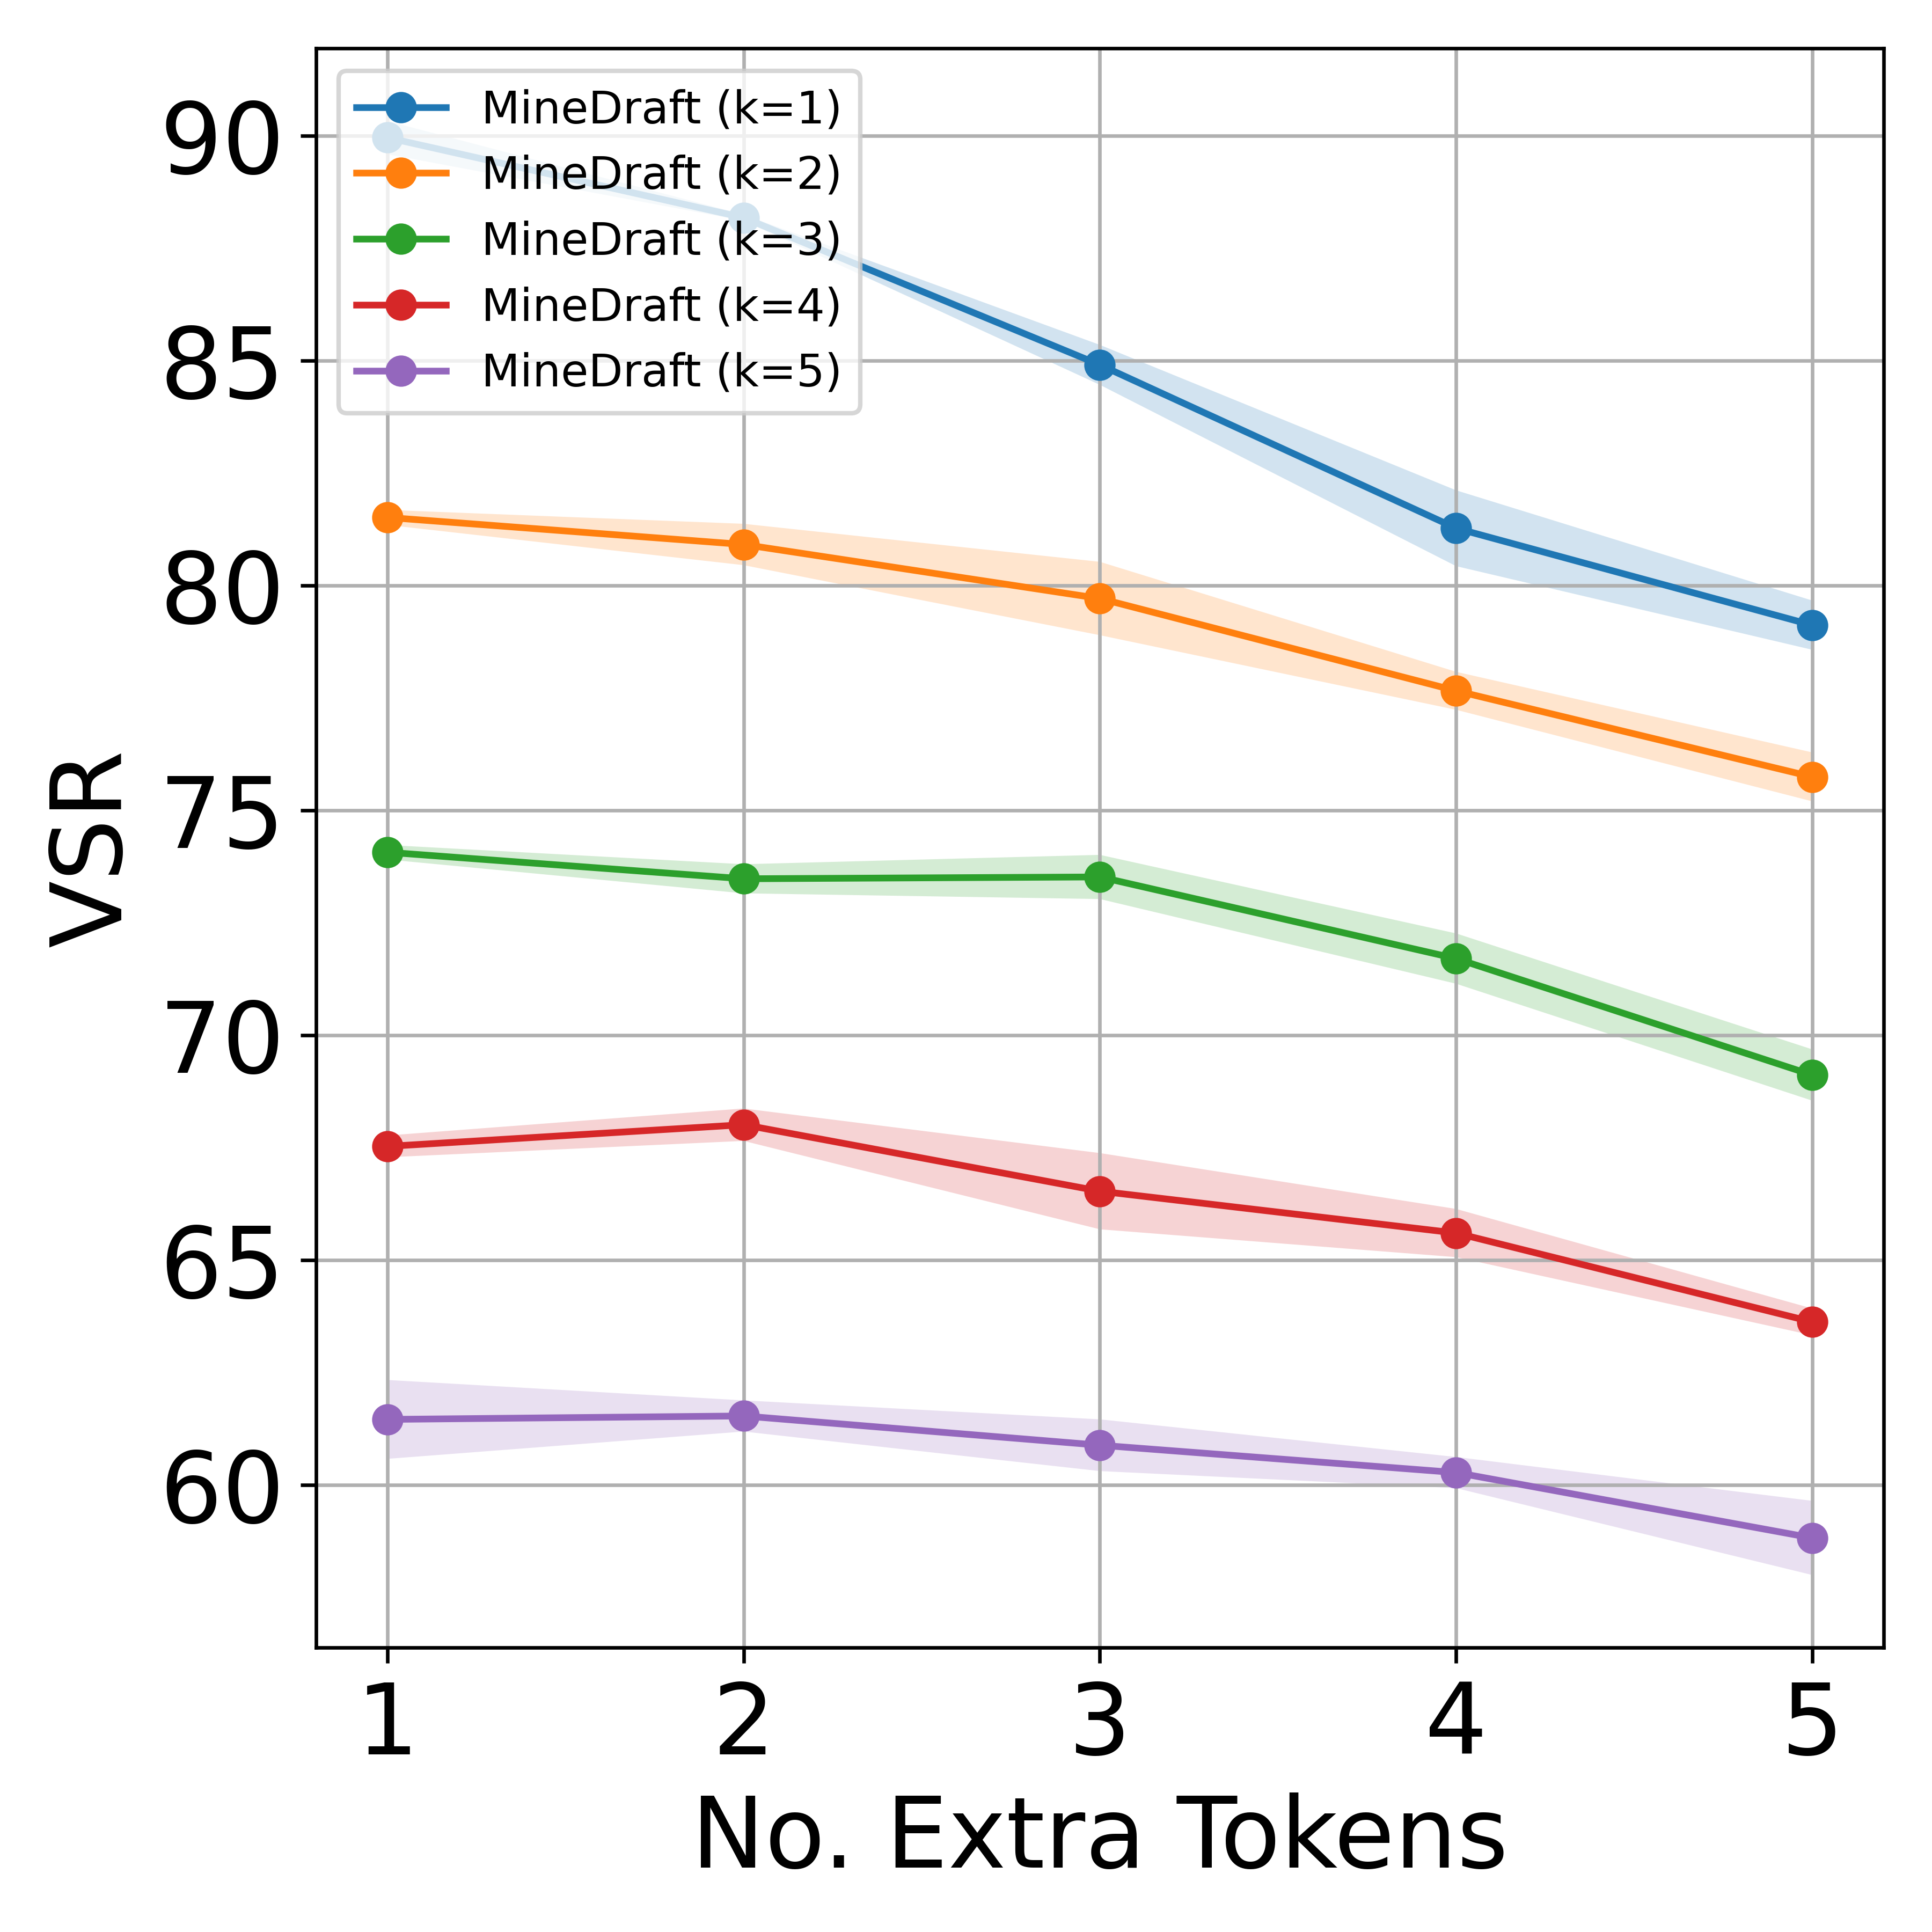
\includegraphics[width=0.23\linewidth]{results/Spec-Bench_Meta-Llama-3_3-70B-Instruct-AWQ-INT4_Llama-3_1-8B-Instruct_160_bs64_n2_100pct_vsr_vs_e.png} &
        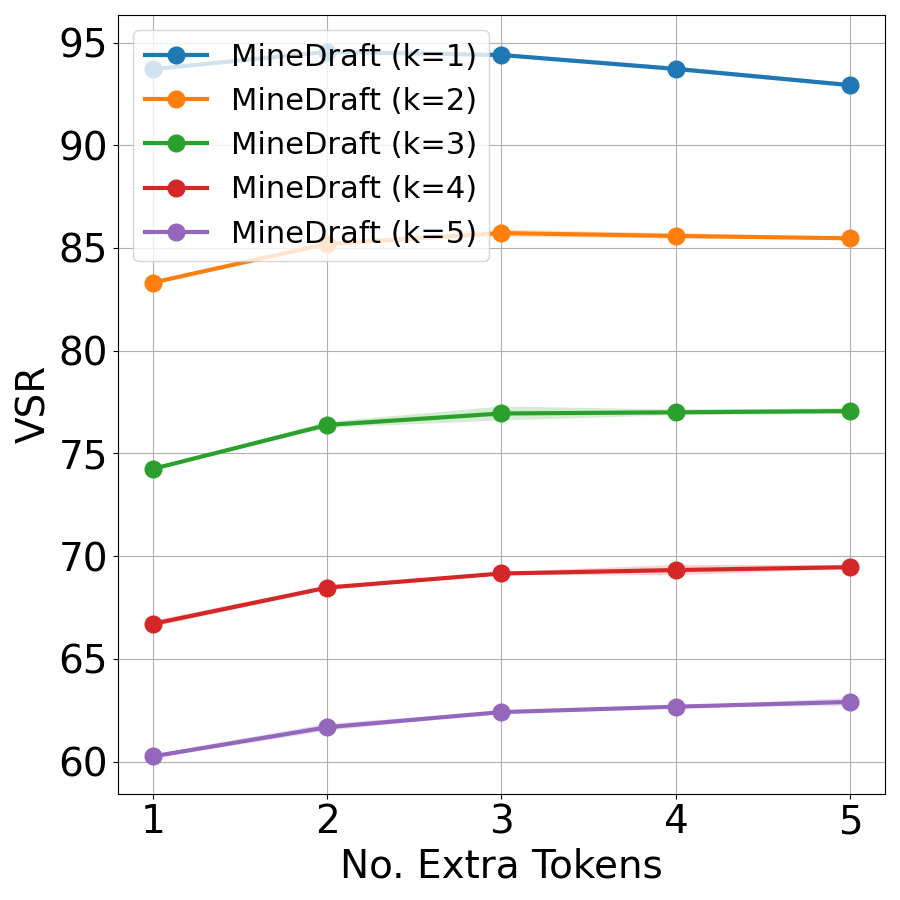
\includegraphics[width=0.23\linewidth]{results/Tough_Meta-Llama-3_3-70B-Instruct-AWQ-INT4_Llama-3_1-8B-Instruct_1000_bs64_n2_100pct_vsr_vs_e.png} \\

    \end{tabular}}
    \caption{VSR comparison for \alg{} with TETRIS across model settings 1 and 5 on $n = 2$ and $\text{temperature} = 0.8$.    
    }
    \label{fig:vsr-vs-e-n2}
\end{figure*}


\begin{figure*}[!ht]
    \centering
    \setlength{\tabcolsep}{1pt} 
    \resizebox{0.99\linewidth}{!}{
    \begin{tabular}{ccccc}
        & \hspace{8mm}\textbf{Arena} & \hspace{8mm}\textbf{ShareGPT} & \hspace{8mm}\textbf{Spec-Bench}  & \hspace{8mm}\textbf{Tough}\\

        \rotatebox{90}{\parbox{3.5cm}{\centering \hspace{10mm}\textbf{$e = 1$}}} &
        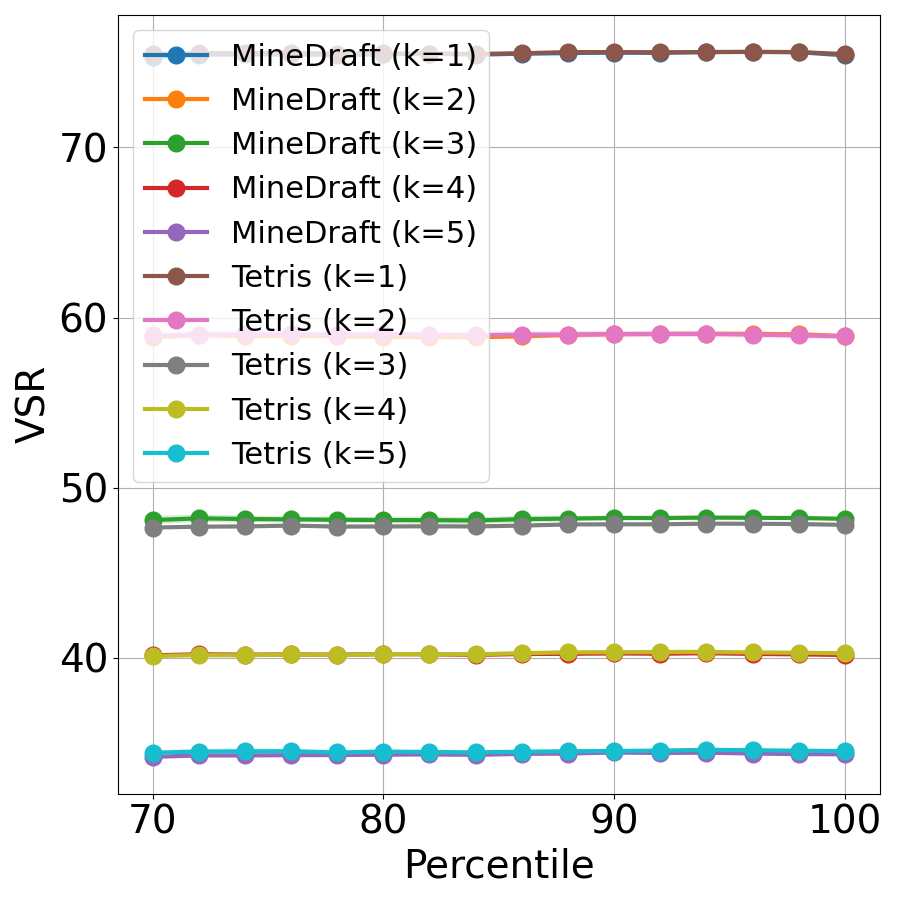
\includegraphics[width=0.23\linewidth]{results/Arena_Qwen3-32B_Qwen3-0_6B_1000_bs16_n2_e1_vsr_vs_percentage.png} &
        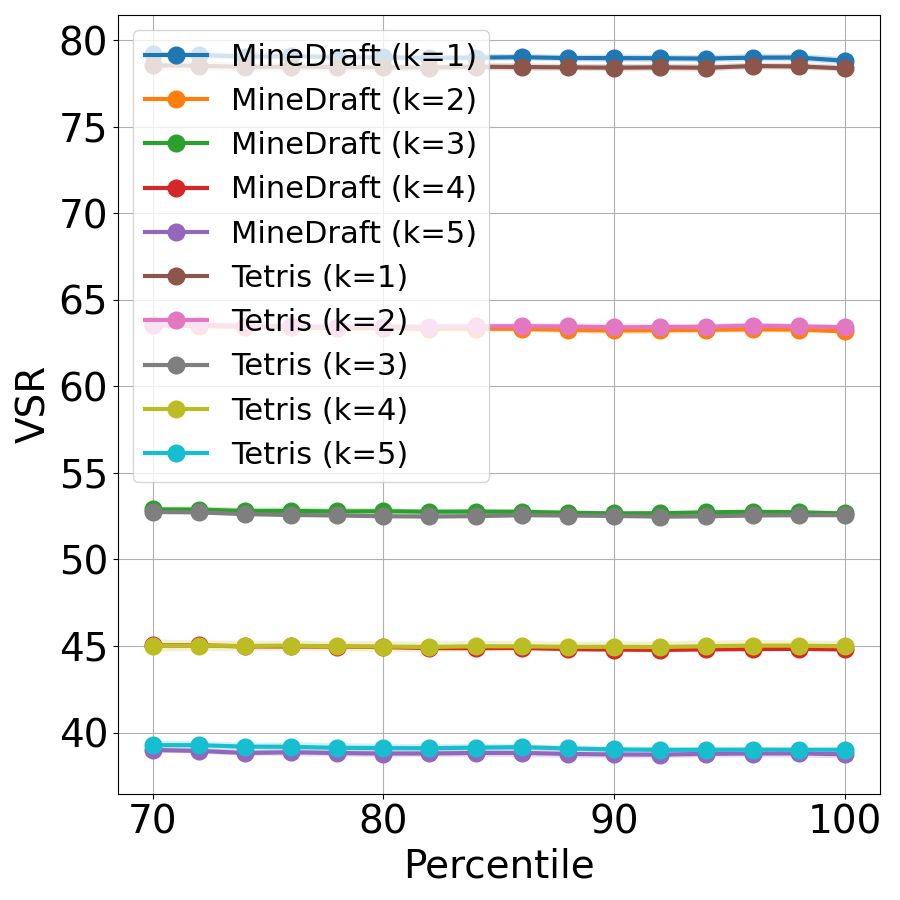
\includegraphics[width=0.23\linewidth]{results/ShareGPT_Qwen3-32B_Qwen3-0_6B_1000_bs16_n2_e1_vsr_vs_percentage.png} &
        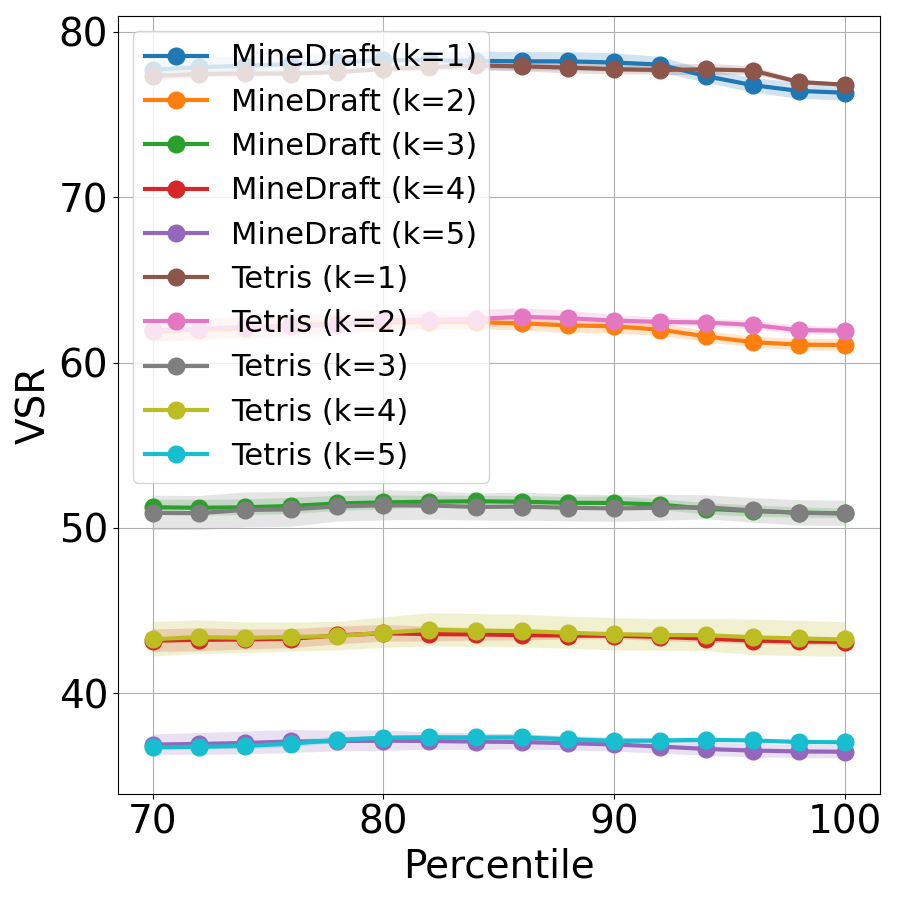
\includegraphics[width=0.23\linewidth]{results/Spec-Bench_Qwen3-32B_Qwen3-0_6B_161_bs16_n2_e1_vsr_vs_percentage.png} &
        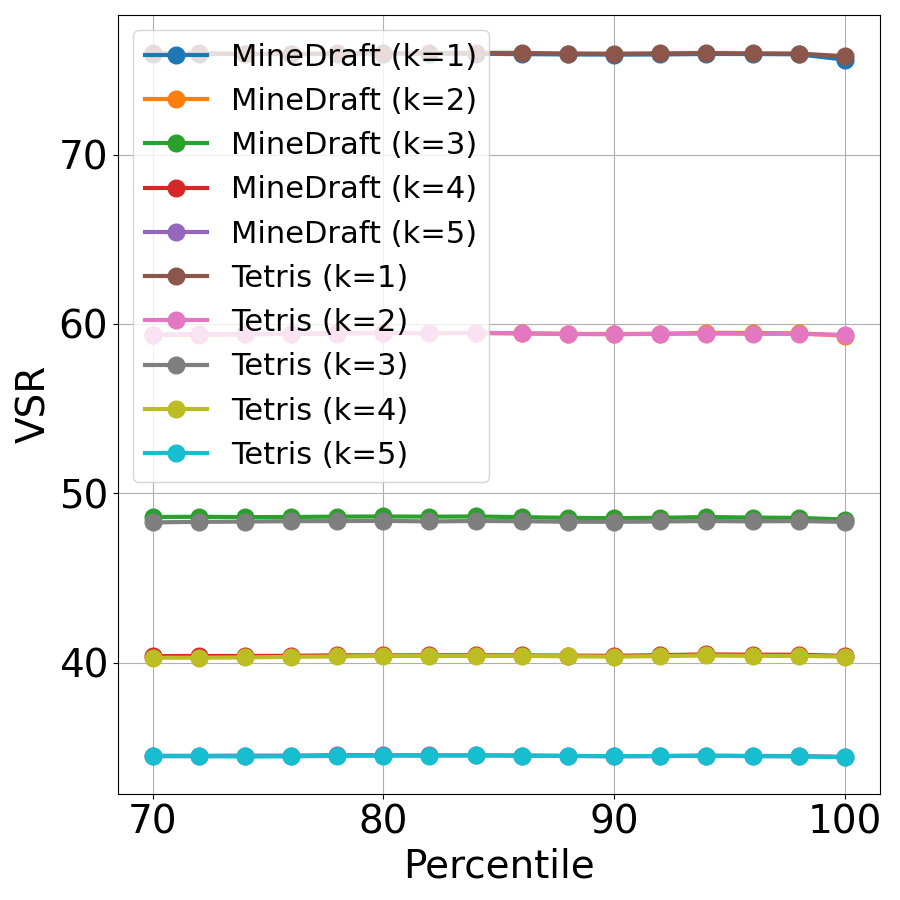
\includegraphics[width=0.23\linewidth]{results/Tough_Qwen3-32B_Qwen3-0_6B_1000_bs16_n2_e1_vsr_vs_percentage.png} \\

        \rotatebox{90}{\parbox{3.5cm}{\centering \hspace{10mm}\textbf{$e = 2$}}} &
        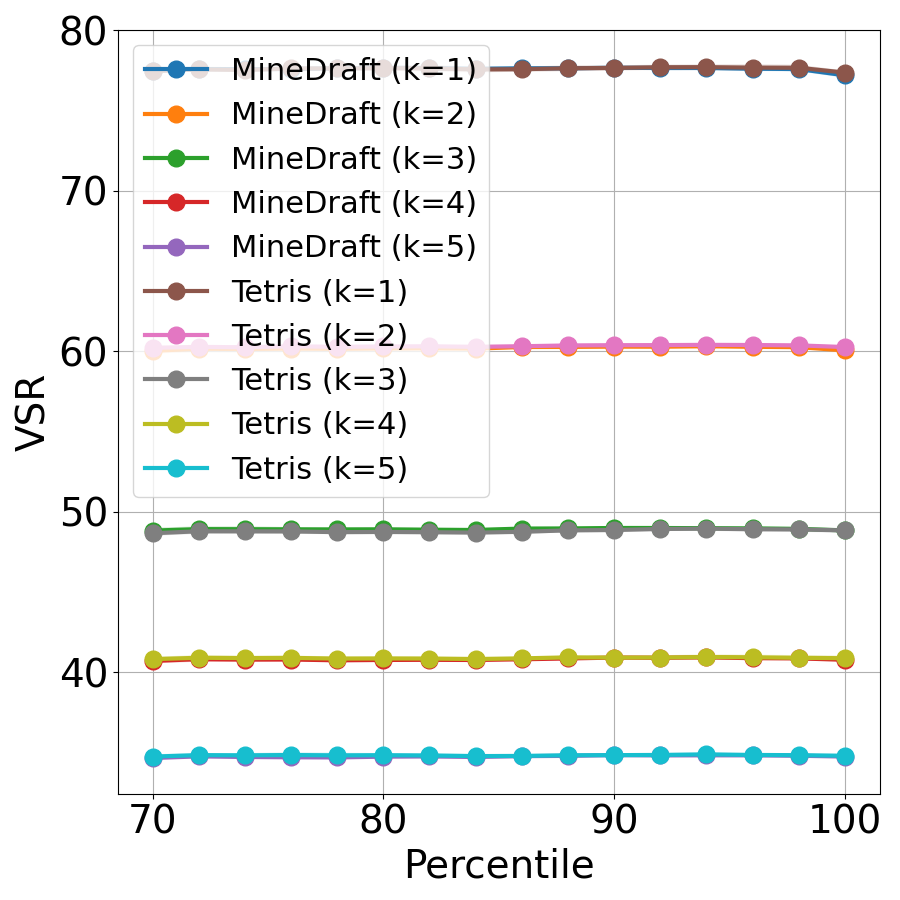
\includegraphics[width=0.23\linewidth]{results/Arena_Qwen3-32B_Qwen3-0_6B_1000_bs16_n2_e2_vsr_vs_percentage.png} &
        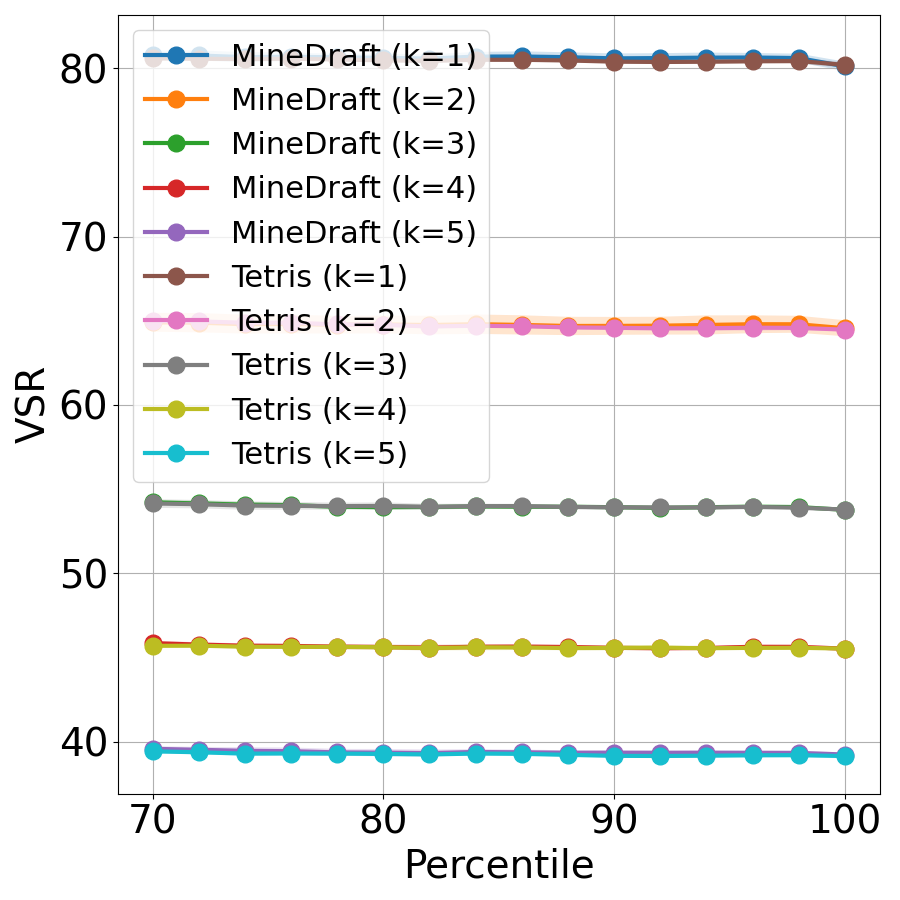
\includegraphics[width=0.23\linewidth]{results/ShareGPT_Qwen3-32B_Qwen3-0_6B_1000_bs16_n2_e2_vsr_vs_percentage.png} &
        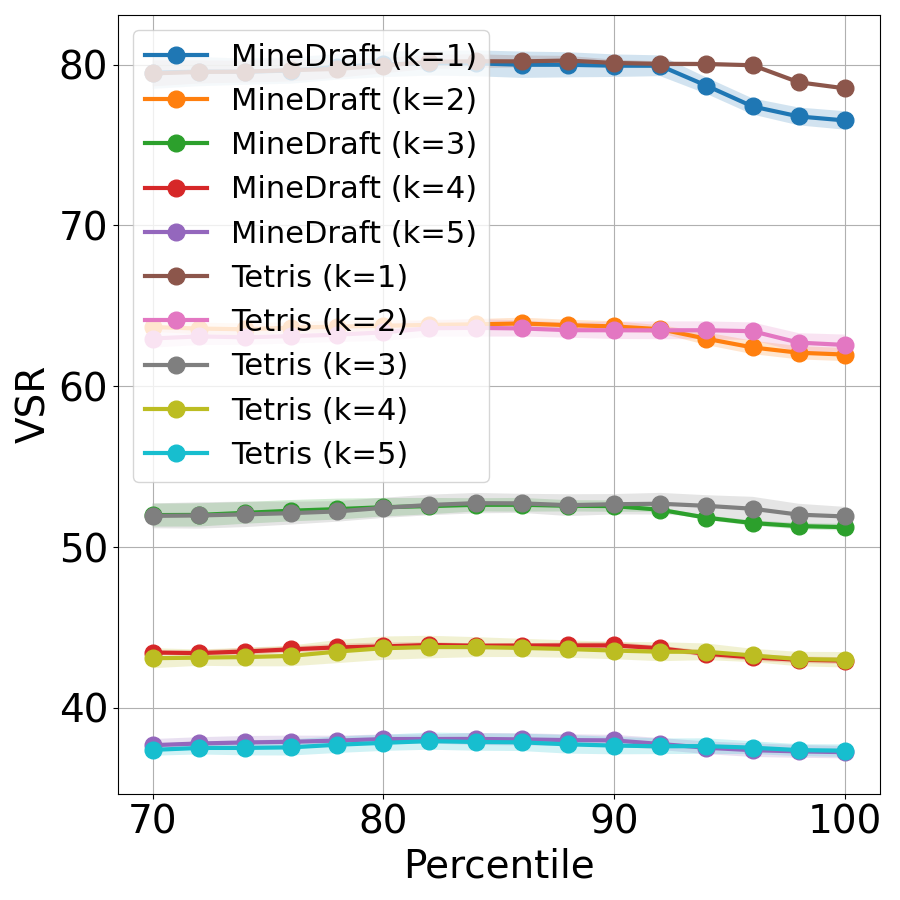
\includegraphics[width=0.23\linewidth]{results/Spec-Bench_Qwen3-32B_Qwen3-0_6B_161_bs16_n2_e2_vsr_vs_percentage.png} &
        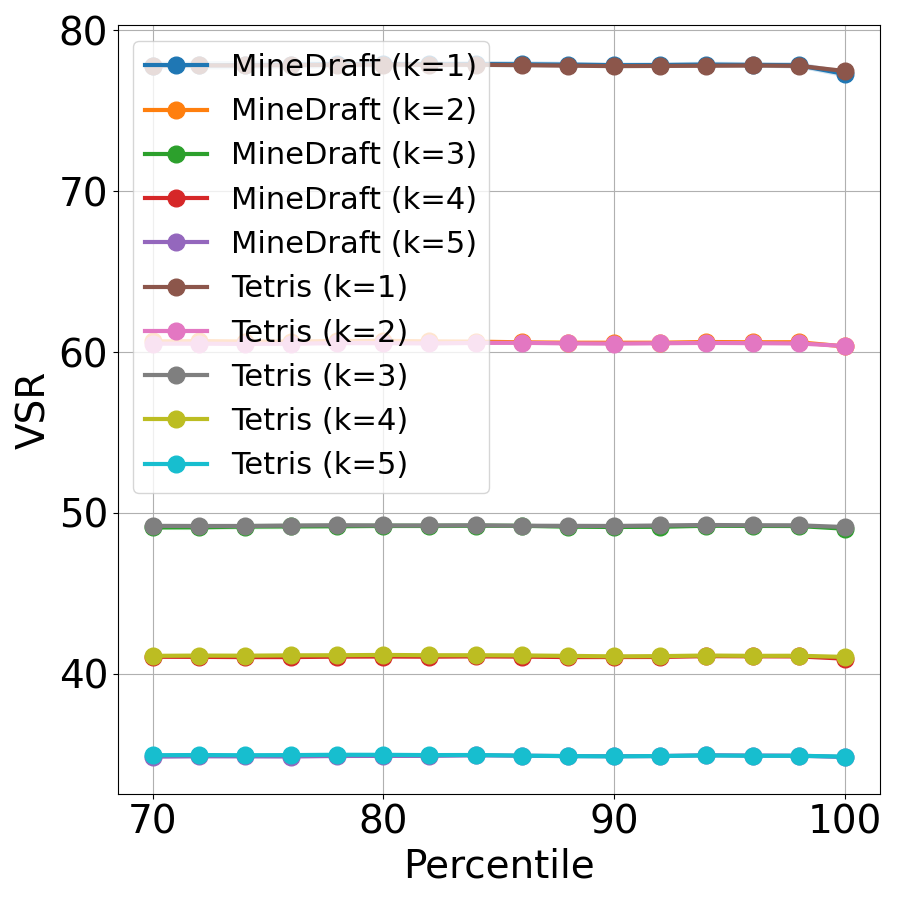
\includegraphics[width=0.23\linewidth]{results/Tough_Qwen3-32B_Qwen3-0_6B_1000_bs16_n2_e2_vsr_vs_percentage.png} \\
    \end{tabular}}
    \caption{VSR comparison for \alg{} with TETRIS and standalone TETRIS across trimming percentiles on model setting 1, $n = 2$ and $\text{temperature} = 0.8$.    
    }
    \label{fig:vsr-vs-percentile-n2}
\end{figure*}


\begin{figure*}[!ht]
    \centering
    \setlength{\tabcolsep}{1pt} 
    \resizebox{0.99\linewidth}{!}{
    \begin{tabular}{ccccc}
        & \hspace{8mm}\textbf{Arena} & \hspace{8mm}\textbf{ShareGPT} & \hspace{8mm}\textbf{Spec-Bench}  & \hspace{8mm}\textbf{Tough}\\
        
        \rotatebox{90}{\parbox{3.5cm}{\centering \hspace{8mm}\textbf{Throughput}}} & 
        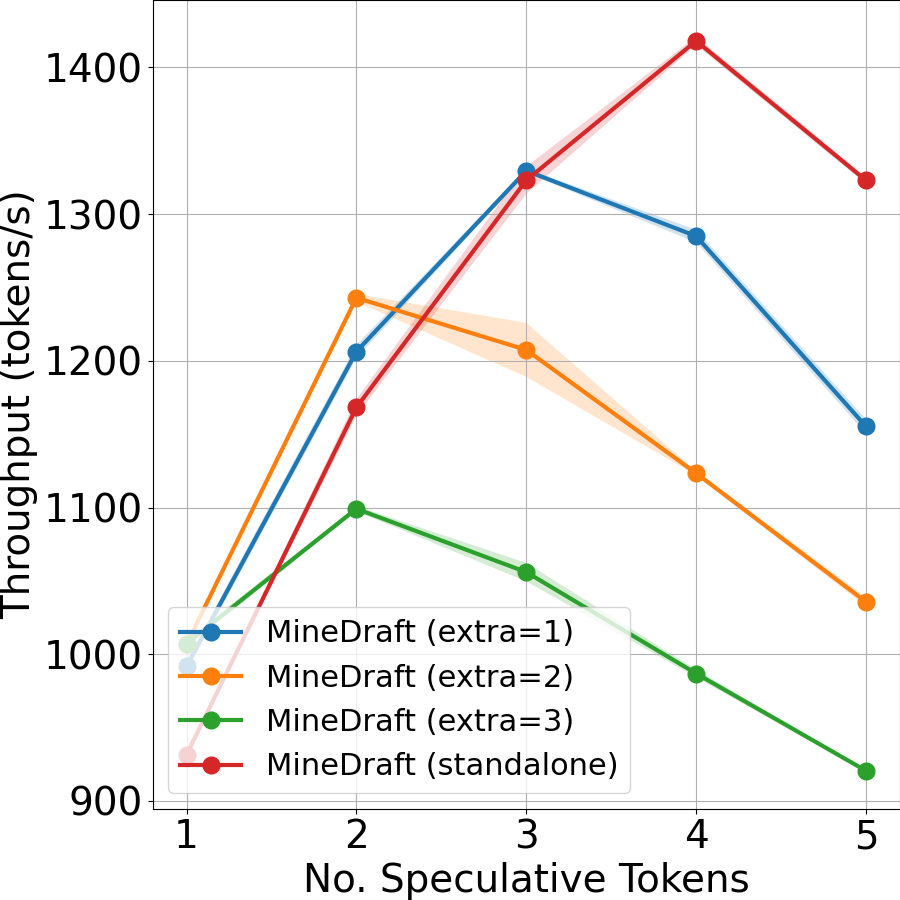
\includegraphics[width=0.23\linewidth]{results/Arena_Qwen3-235B-A22B-Instruct-2507-FP8_Qwen3-14B_1000_bs64_n2_100pct_gen_throughput.png} &
        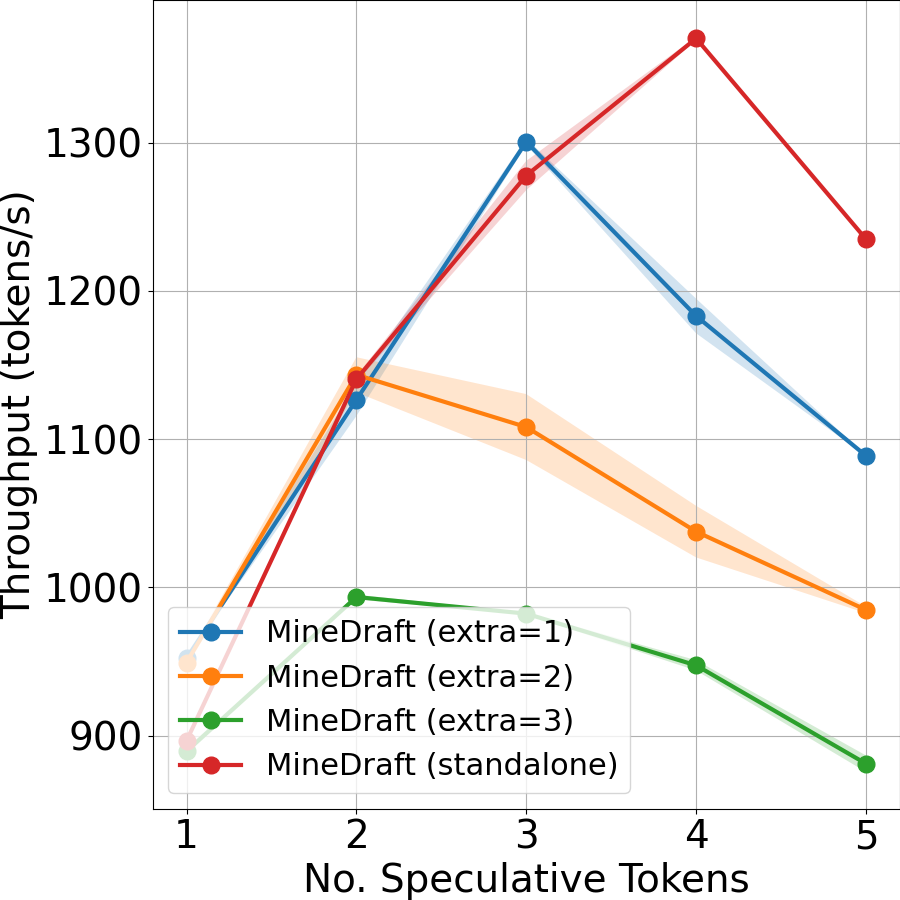
\includegraphics[width=0.23\linewidth]{results/ShareGPT_Qwen3-235B-A22B-Instruct-2507-FP8_Qwen3-14B_1000_bs64_n2_100pct_gen_throughput.png} &
        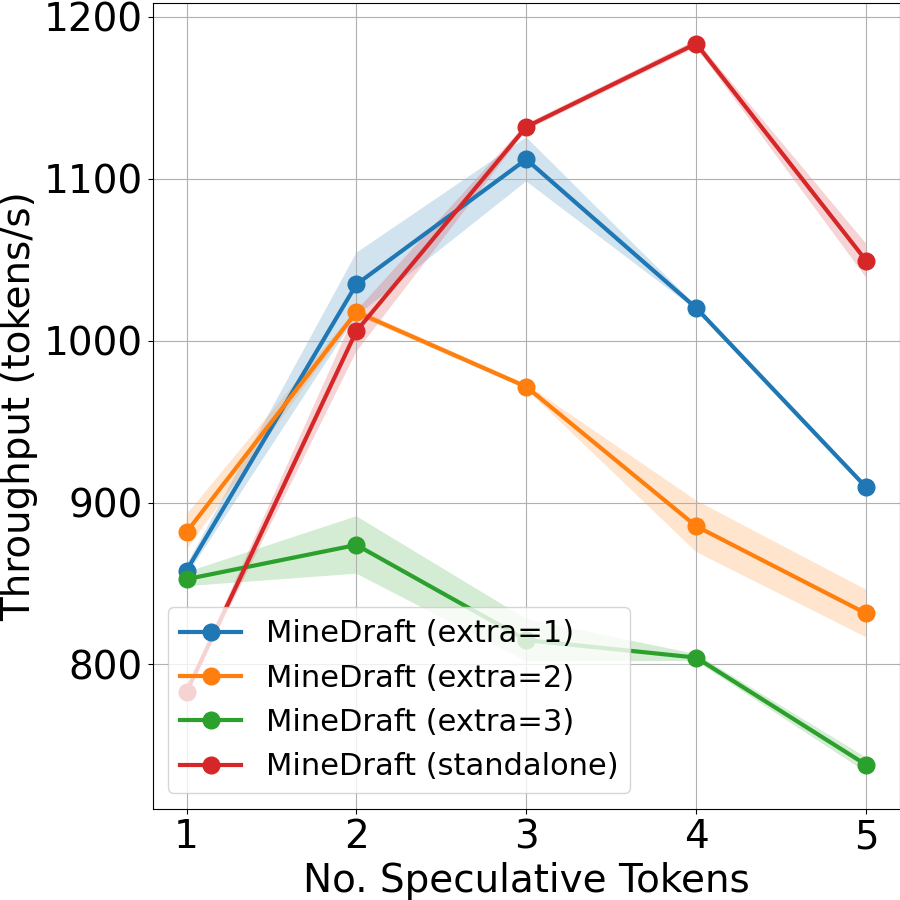
\includegraphics[width=0.23\linewidth]{results/Spec-Bench_Qwen3-235B-A22B-Instruct-2507-FP8_Qwen3-14B_161_bs64_n2_100pct_gen_throughput.png} &
        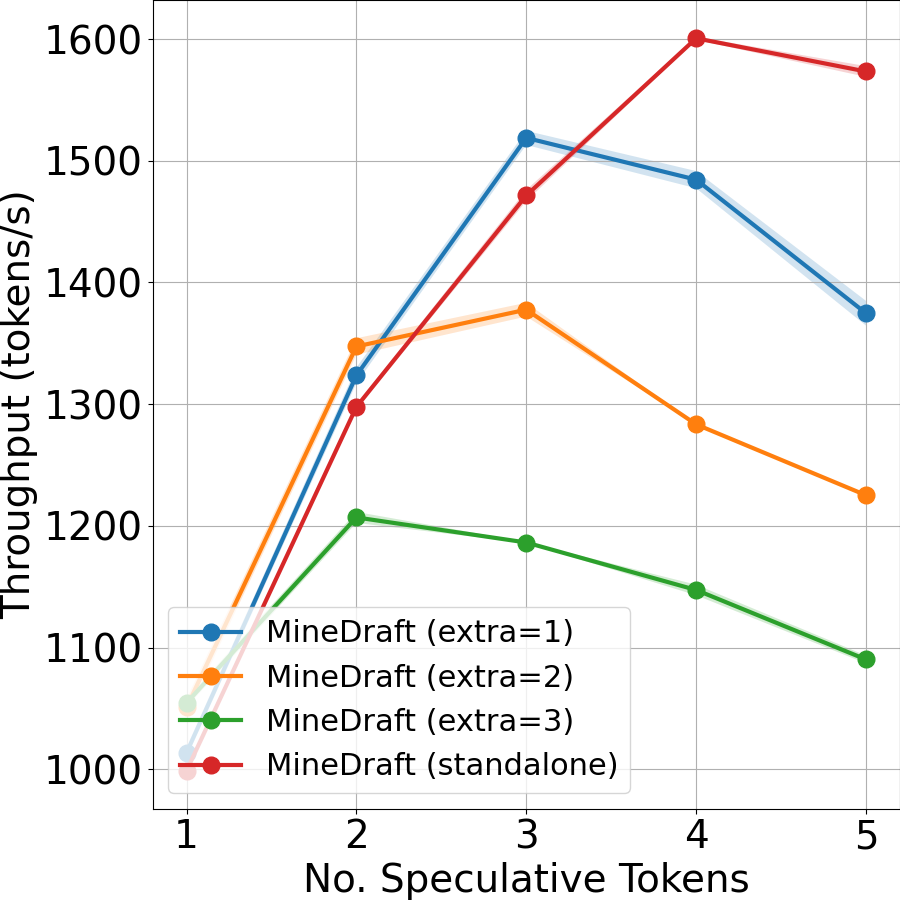
\includegraphics[width=0.23\linewidth]{results/Tough_Qwen3-235B-A22B-Instruct-2507-FP8_Qwen3-14B_1000_bs64_n2_100pct_gen_throughput.png} \\

        \rotatebox{90}{\parbox{3.5cm}{\centering \hspace{8mm}\textbf{E2EL}}} & 
        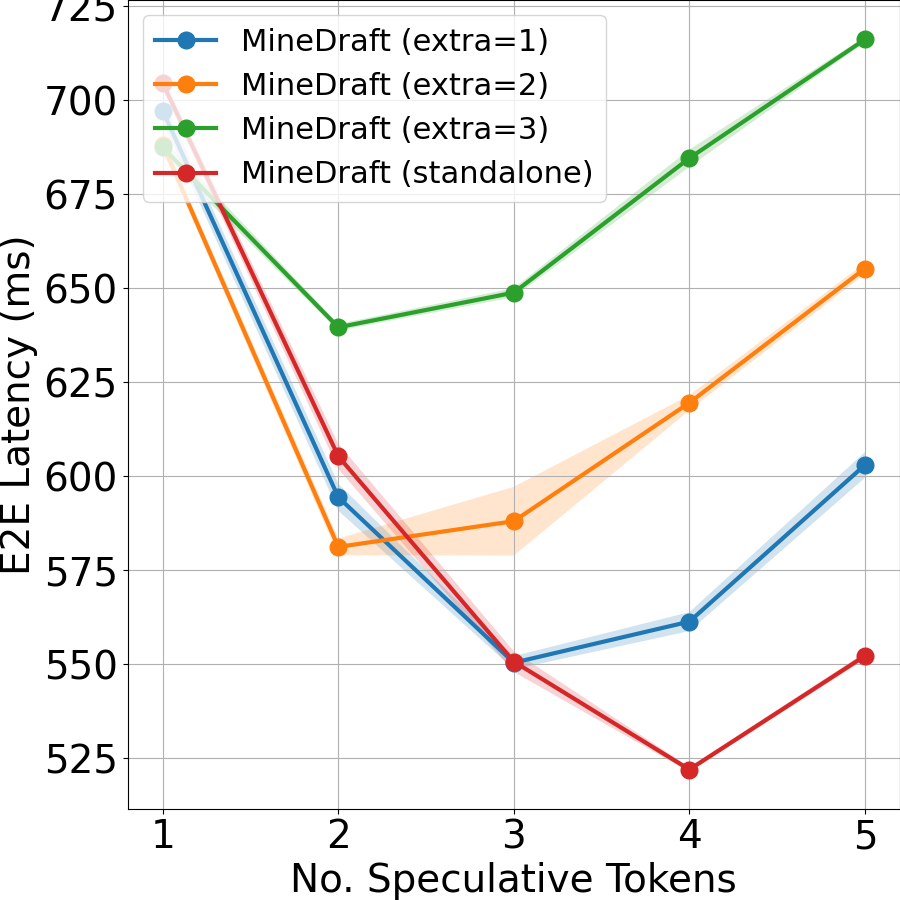
\includegraphics[width=0.23\linewidth]{results/Arena_Qwen3-235B-A22B-Instruct-2507-FP8_Qwen3-14B_1000_bs64_n2_100pct_latency.png} &
        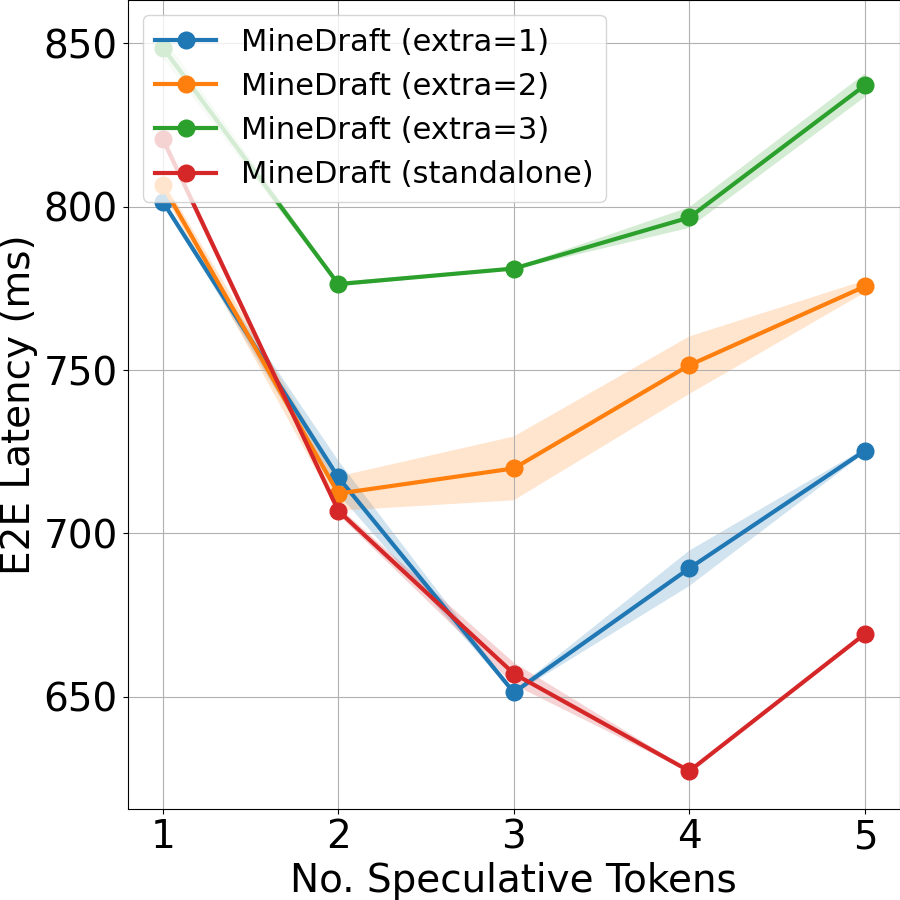
\includegraphics[width=0.23\linewidth]{results/ShareGPT_Qwen3-235B-A22B-Instruct-2507-FP8_Qwen3-14B_1000_bs64_n2_100pct_latency.png} &
        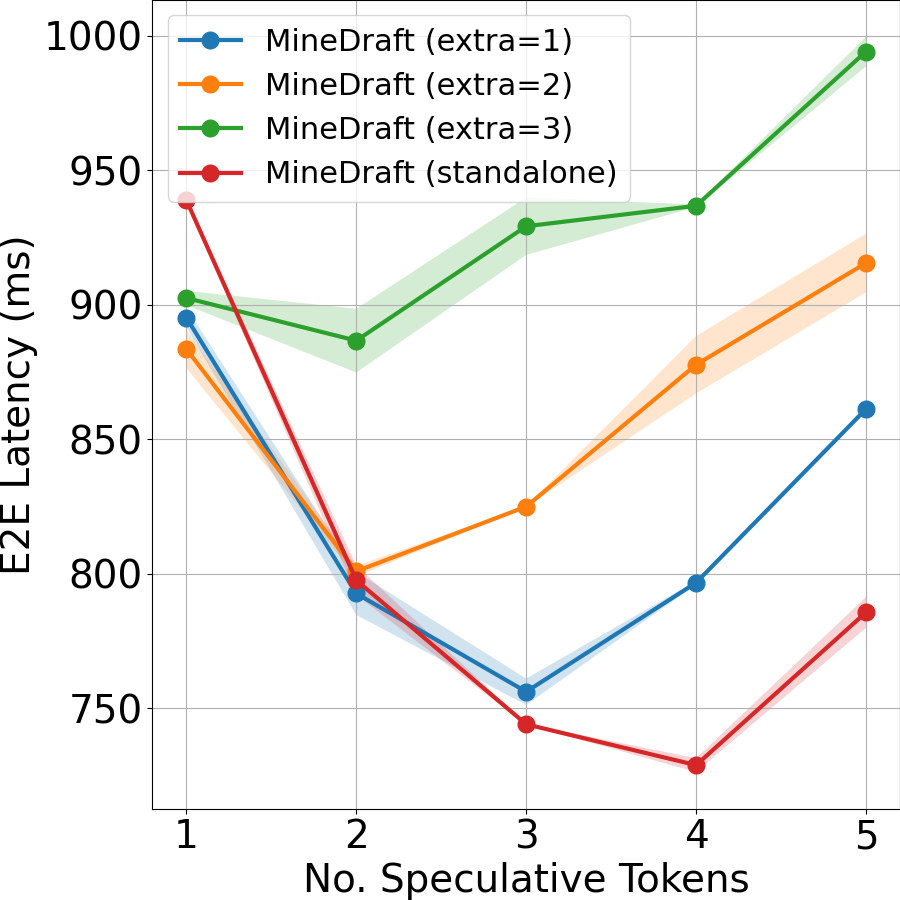
\includegraphics[width=0.23\linewidth]{results/Spec-Bench_Qwen3-235B-A22B-Instruct-2507-FP8_Qwen3-14B_161_bs64_n2_100pct_latency.png} &
        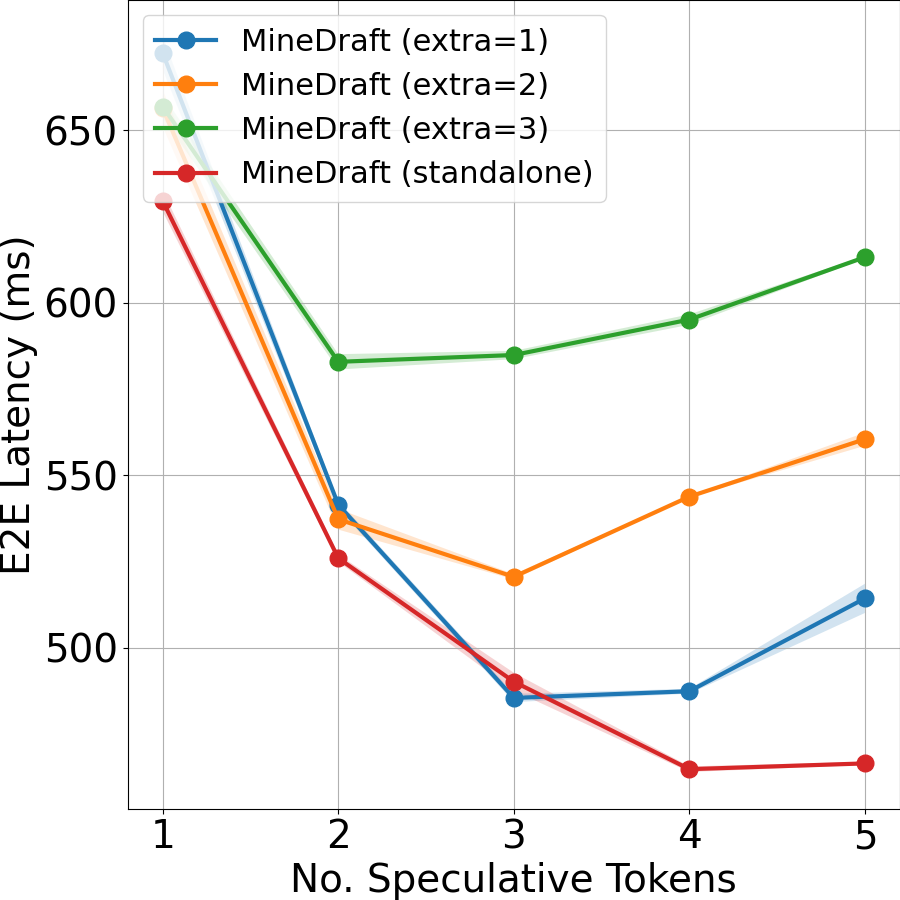
\includegraphics[width=0.23\linewidth]{results/Tough_Qwen3-235B-A22B-Instruct-2507-FP8_Qwen3-14B_1000_bs64_n2_100pct_latency.png} \\
    \end{tabular}}
    \caption{\alg{} Throughput and End-to-End Latency (ms) results on Qwen3-235B-A22B-Instruct-2507-FP8 paired with Qwen3-13B, $n=2$ and $\text{temperature}=0.8$. The reported numbers reflect the mean and standard deviation over 2 independent trials.    }
    \label{fig:exp-qwen-235b}
\end{figure*}


\subsection{Performance Improvement Metrics.}
\label{app:performance_improvement}
% \para{Performance improvement metrics.} 
To quantify the performance improvements of \alg{}, we compute two percentage metrics relative to baseline methods. Let $p$ denote a performance metric, and let $B_p(k)$ denote the best value of $p$ achieved by baseline methods at $k$, where $k$ is the number of draft tokens per step. Similarly, let $M_p(k)$ denote the best value of $p$ achieved by \alg{} variants (including the standalone variant and its integration with TETRIS) at $k$.

\para{Average improvement over the best baseline.} 
First, for each performance metric $p$, the optimal baseline draft token count $k_p^*$ is selected as follows:
\begin{itemize}
    \item If $p$ is \textbf{maximized} (higher is better): $k_p^*=\arg\max\limits_k B_p(k).$

    \item If $p$ is \textbf{minimized} (lower is better):
    $
    k_p^*=\arg\min\limits_k B_p(k).
    $
\end{itemize}
Let $B_p^* = B_p(k_p^*)$ be the corresponding baseline performance metric value. Next, among all \alg{} variants, select the best \alg{} performance metric value at $k_p^*$ as $M_p^* = M_p(k_p^*)$. The average improvement of $p$ of \alg{} over the best baseline method $\uparrow_p$ (in percent) is calculated as follows:
\begin{itemize}
    \item If $p$ is \textbf{maximized}:
    $
    \uparrow_p=\frac{M_p^*-B_p^*}{B_p^*}\times 100.
    $
    \item If $p$ is \textbf{minimized}:
    $
    \uparrow_p=\frac{B_p^*-M_p^*}{B_p^*}\times 100.
    $
\end{itemize}

\para{Maximum average improvement.}
Define $S_p(k)$ as the value of $p$ of standard SD or EAGLE*~\citep{li2024eagle,li2024eagle2,li2025eagle3}, where applicable, at $k$. For a given target metric $p$, the average percentage improvement of \alg{} over standard SD at $k$ ($\Delta_p(k)$) is calculated as:
\begin{itemize}
    \item If $p$ is \textbf{maximized}:
    $
    \Delta_p(k)=\frac{M_p(k)-S_p(k)}{S_p(k)}\times 100.
    $
    \item If $p$ is \textbf{minimized}:
    $
    \Delta_p(k)=\frac{S_p(k)-M_p(k)}{S_p(k)}\times 100.
    $
\end{itemize}
The maximum average percentage improvement of $p$ of \alg{} over standard SD or EAGLE ($\Delta_p$) is the maximum of $\Delta_p(k)$ over all $k$ values:
$
\Delta_p=\max\limits_k \Delta_p(k).
$



\subsection{End-to-End Latency Results}
\label{app:exp-e2el}

\para{Comparison with baselines.} 
\cref{fig:e2elatencty-baseline} shows that \alg{} reduces end-to-end latency by up to 31.13\% relative to the best-performing baseline. The maximum reduction compared to standard SD reaches 39.51\%, consistent with the theoretical analysis in \cref{sec:theoretical_analysis}, which predicts a minimum improvement of 37\%.

\para{Results with larger draft model.}
As shown in \cref{fig:e2elatencty-qwen8b}, under model setting 4 with Qwen3-8B as the draft model, \alg{} achieves its lowest end-to-end latency when generating 1--2 draft tokens per step. Drafting more than two tokens per step leads to degraded performance. In this setting, integrating TETRIS does not yield additional reductions in end-to-end latency, as the computational cost of drafting already dominates that of verification. Standard SD fails to execute on this setting due to VRAM constraints. The effect of draft model size on performance is further examined in \cref{app:exp-draft-model}.


\para{Integration with different drafting strategies.}
\cref{fig:e2elatencty-strategy} shows that \alg{} achieves a 15.67\% reduction in end-to-end latency relative to the best standard SD result on Setting~5, with a maximum improvement of 20.63\%. On the selected EAGLE model settings, \alg{} outperforms the best standalone EAGLE result by up to 6.47\% and attains a maximum latency reduction of 16.30\%.


\subsection{Ablation on Draft Model Size}
\label{app:exp-draft-model}
We fix the target model to Qwen3-32B and evaluate \alg{} using three draft models: Qwen3-0.6B, Qwen3-1.7B, and Qwen3-4B. As shown in \cref{fig:qwen3-32b-draft-models}, performance degrades noticeably when the number of draft tokens per step exceeds $3$ for the Qwen3-4B and Qwen3-0.6B draft models, whereas the medium-sized Qwen3-1.7B model is less affected.

These results highlight the need to balance draft quality and speed in \alg{}. An overly small draft model (e.g., Qwen3-0.6B) may fail to generate sufficiently accurate drafts, leading to a low verification success rate and degraded performance. Conversely, an overly large draft model (e.g., Qwen3-4B), while capable of producing high-quality drafts, may generate them too slowly to benefit from PSD, which requires drafting to be faster than verification. As shown in \cref{fig:qwen3-32b-draft-models}, Qwen3-1.7B strikes this balance by producing accurate drafts at sufficient speed to exploit parallelized drafting in \alg{}. This observation is further supported by Nsight~\citep{NVIDIA_Nsight_Systems_2024} profiling with Spec-Bench in \cref{app:nsight}.


\subsection{Empirical Results with Varied Sequences per Request and Batch Sizes.}
\label{app:exp-n-m}
Using Setting~1, we evaluate \alg{} across varying numbers of sequences per request ($n$) and batch sizes ($m$). As shown in \cref{fig:throughput-n,fig:e2elatencty-n,fig:throughput-bs,fig:e2elatencty-bs}, \alg{} consistently improves both average throughput and end-to-end latency over standard SD across all tested configurations of $n$ and $m$. Specifically, varying $n$, \alg{} achieves up to 72.64\% improvement in throughput and 38.41\% reduction in latency; varying $m$, the corresponding improvements reach 75.81\% and 40.79\%. 

As shown in \cref{fig:throughput-bs,fig:e2elatencty-bs}, when the number of draft tokens per step reaches five, the performance of \alg{} becomes comparable to that of standard SD with a doubled batch size ($2m$). This result highlights the effectiveness of \alg{} as a batch PSD framework: with appropriate adaptive drafting strategies and model configurations, \alg{} can further optimize performance even when a large number of draft tokens are generated per step.


\subsection{Analysis of Verification Success Rate}
\label{app:exp-vsr}

The verification success rate (VSR) is defined as follows:
\eqs{
    \textstyle \textit{VSR} = \frac{\textit{Accepted tokens}}{\textit{Tokens sent for verification}} \ ,    
}
which is the proportion of tokens successfully verified out of the total number of tokens submitted for verification. VSR measures the quality of the selected draft tokens. We analyze the VSR of \alg{} integrated with TETRIS under Settings~1 and~5. As shown in \cref{fig:vsr-vs-e-all,fig:vsr-vs-e-n2}, VSR generally increases with the number of extra tokens, except on the Spec-Bench dataset, where VSR decreases more frequently than on the other datasets.

We attribute this anomaly to the combined effects of Spec-Bench’s smaller sample size and TETRIS’s behavior on non-full batches. Because Spec-Bench contains fewer conversations than the other datasets, its requests are exhausted more quickly, causing both batches to fall below their nominal capacity $m$ earlier in the lifespan of \alg{}. When TETRIS operates on non-full batches, the reduced pool of candidate draft tokens increases the likelihood of selecting lower-quality drafts, which, in turn, raises the target model's rejection rate. As a result, VSR decreases during non-full-batch operation; since a larger fraction of SD steps occur under this regime, the aggregate VSR is negatively affected, effectively diluting the high VSR observed during the initial, fully saturated steps.

To validate this explanation for the VSR degradation observed on Spec-Bench, we compute VSR over truncated portions of the execution, considering only the initial 70\%--100\% or 80\%--100\% of SD steps. As shown in \cref{fig:vsr-vs-percentile-all,fig:vsr-vs-percentile-n2}, on Spec-Bench, the VSR of \alg{} integrated with TETRIS remains comparable to or higher than that of standalone TETRIS until approximately 82--86\% of SD steps for $n=1$, and until approximately 92\% for $n=2$.
In contrast, on the Arena, ShareGPT, and Tough datasets, the VSR of \alg{} with TETRIS matches that of standalone TETRIS over the first 98\% of SD steps for $n=1$, and throughout the entire evaluation for $n=2$.


\subsection{Additional Experiment Results on Larger Models}
\label{app:exp-large-model}
We conduct additional experiments on a large Mixture-of-Experts (MoE) target model~\citep{shazeer2017,dai2024deepseekmoe,qwen3technicalreport}, Qwen3-235B-A22B-Instruct-2507-FP8~\citep{qwen3technicalreport}, to evaluate the compatibility of \alg{} with modern MoE architectures. We use Qwen3-14B~\citep{qwen3technicalreport} as the draft model with $m=64$, $n=2$, and the temperature set to $0.8$, served on five H100 GPUs. Under this configuration, standard SD is infeasible due to VRAM constraints.
As shown in \cref{fig:exp-qwen-235b}, \alg{} achieves its best performance when four draft tokens are generated per step, reaching an average throughput of approximately 1200--1600 tokens per second.


\begin{figure}[!ht]
    \centering
    \small
    \begin{minipage}[t]{0.48\textwidth}
        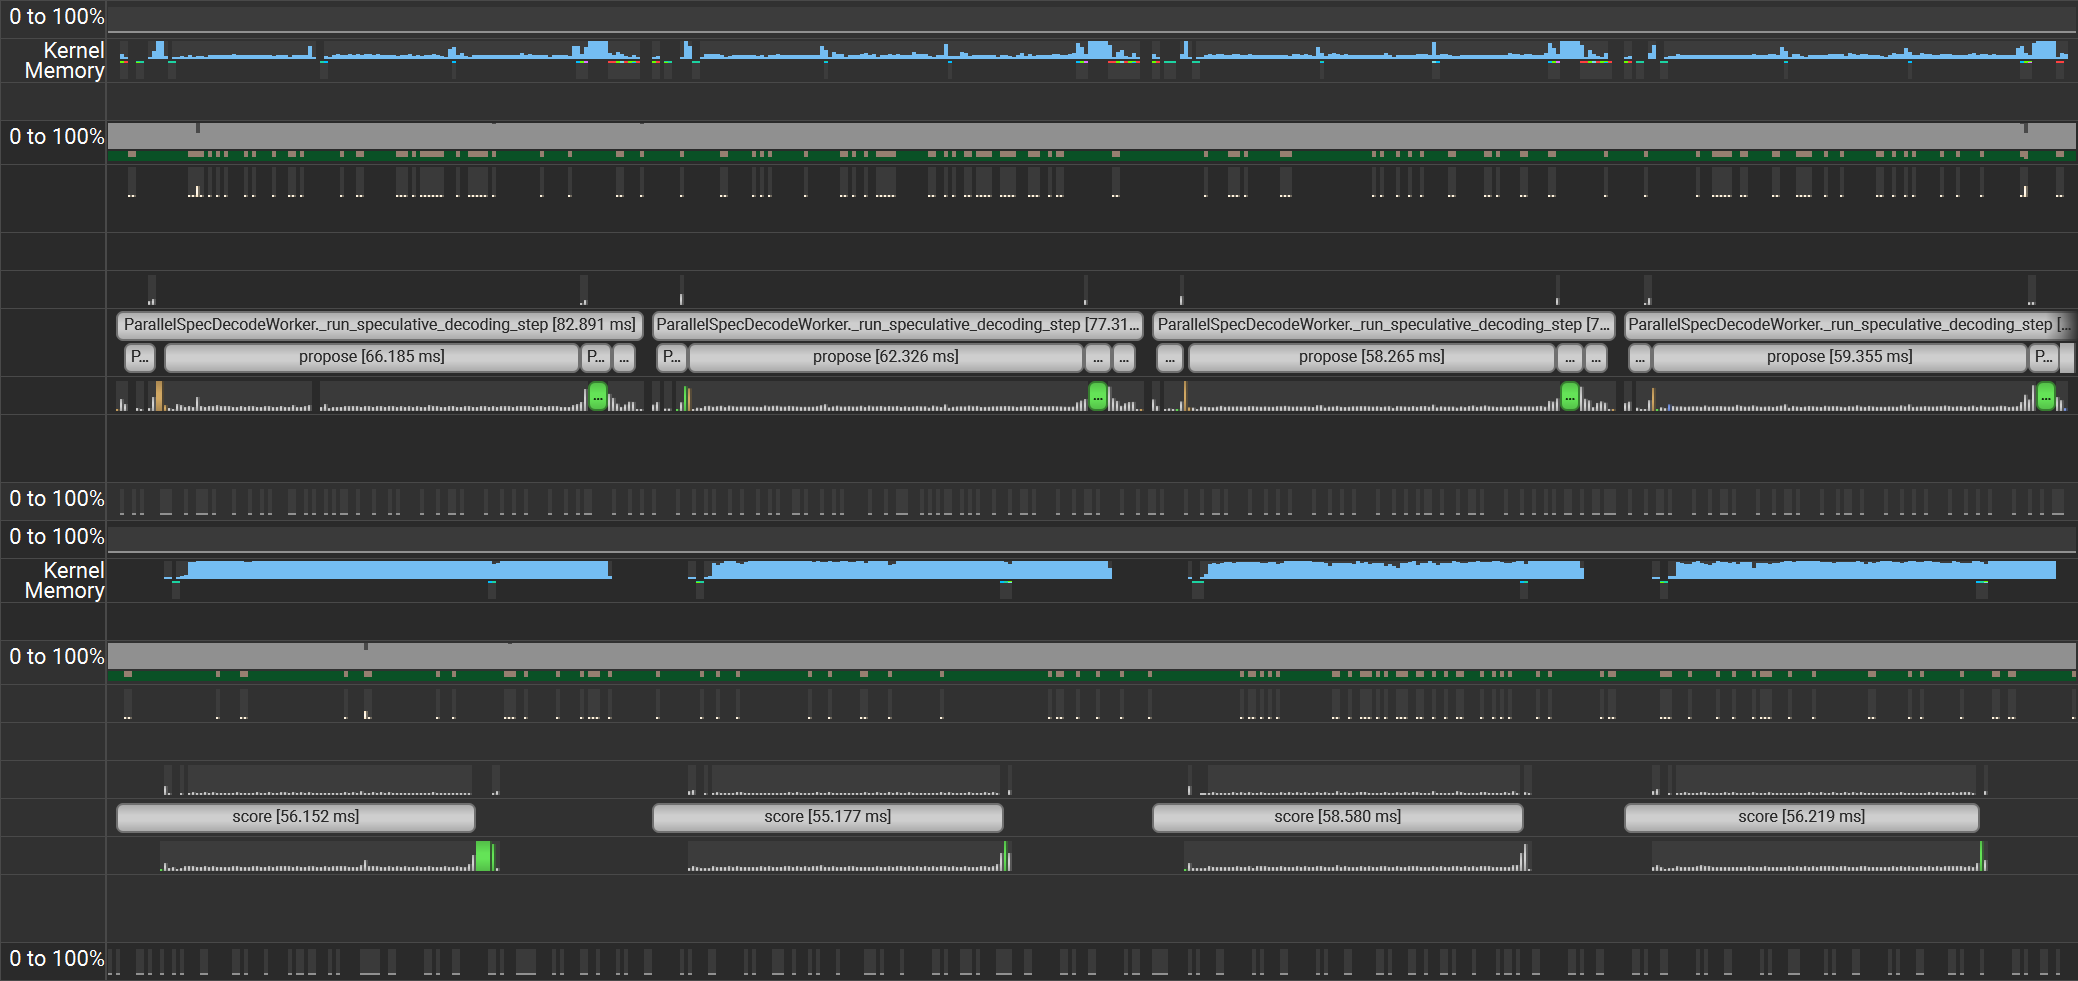
\includegraphics[width=\linewidth, height=0.25\textheight, keepaspectratio]{figures/Qwen3-32B_0.6B_k3.png}
        \par\vspace{5pt}
        \textbf{(a)} Sample segment of Nsight profiling results with model setting 1, Spec-Bench dataset, and $k=3$. Median drafting and verification times are 49.60 ms and 48.62 ms, respectively, suggesting \alg{} almost perfectly overlaps drafting with verification under this configuration.
    \end{minipage}
    \hfill
    \begin{minipage}[t]{0.48\textwidth}
        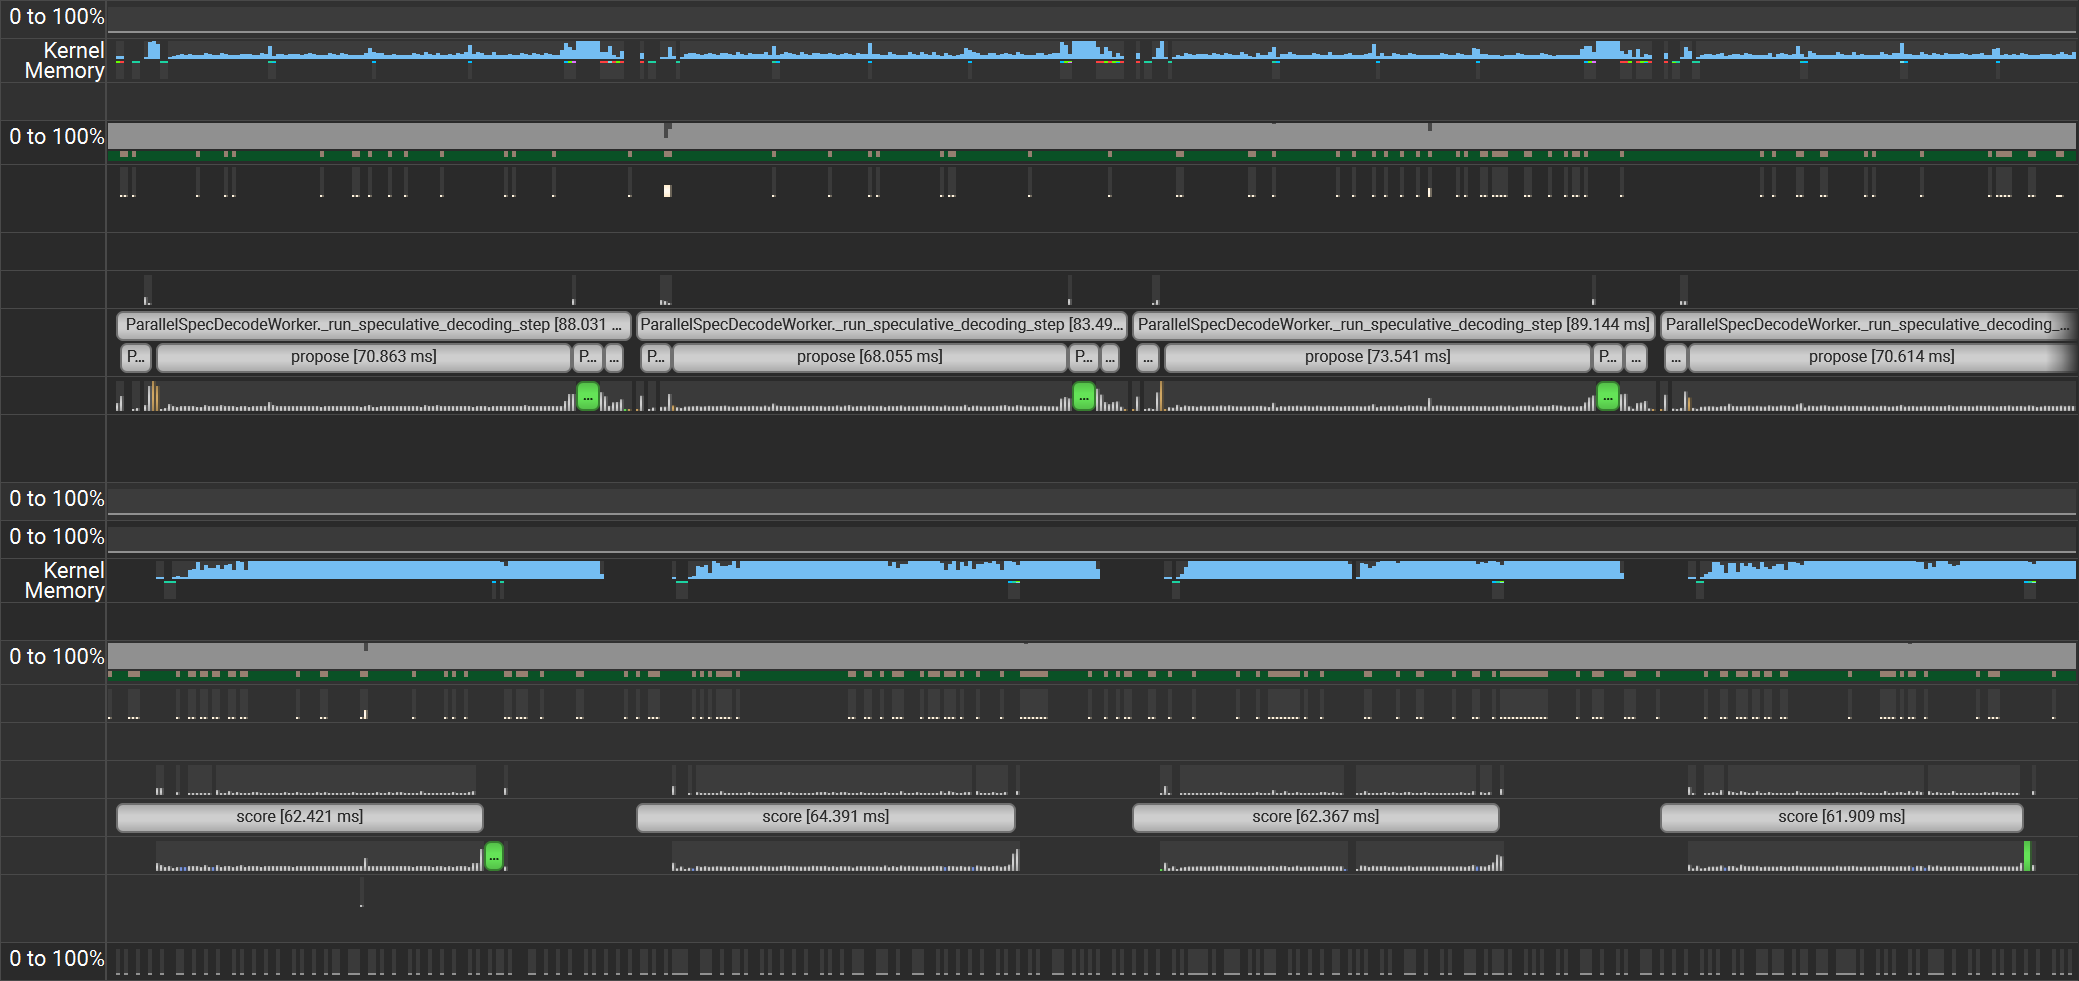
\includegraphics[width=\linewidth, height=0.25\textheight, keepaspectratio]{figures/Qwen3-32B_0.6B_k4.png}
        \par\vspace{5pt}
        \textbf{(b)} Sample segment of Nsight profiling results with model setting 1, Spec-Bench dataset, and $k=4$. Median drafting and verification times are 64.06 ms and 51.06 ms, respectively, suggesting drafting time exceeds verification time by 25.48\%, and the performance of \alg{} may degrade under this configuration.
    \end{minipage}

    \vspace{0.5cm} 
    \begin{minipage}[t]{0.48\textwidth}
        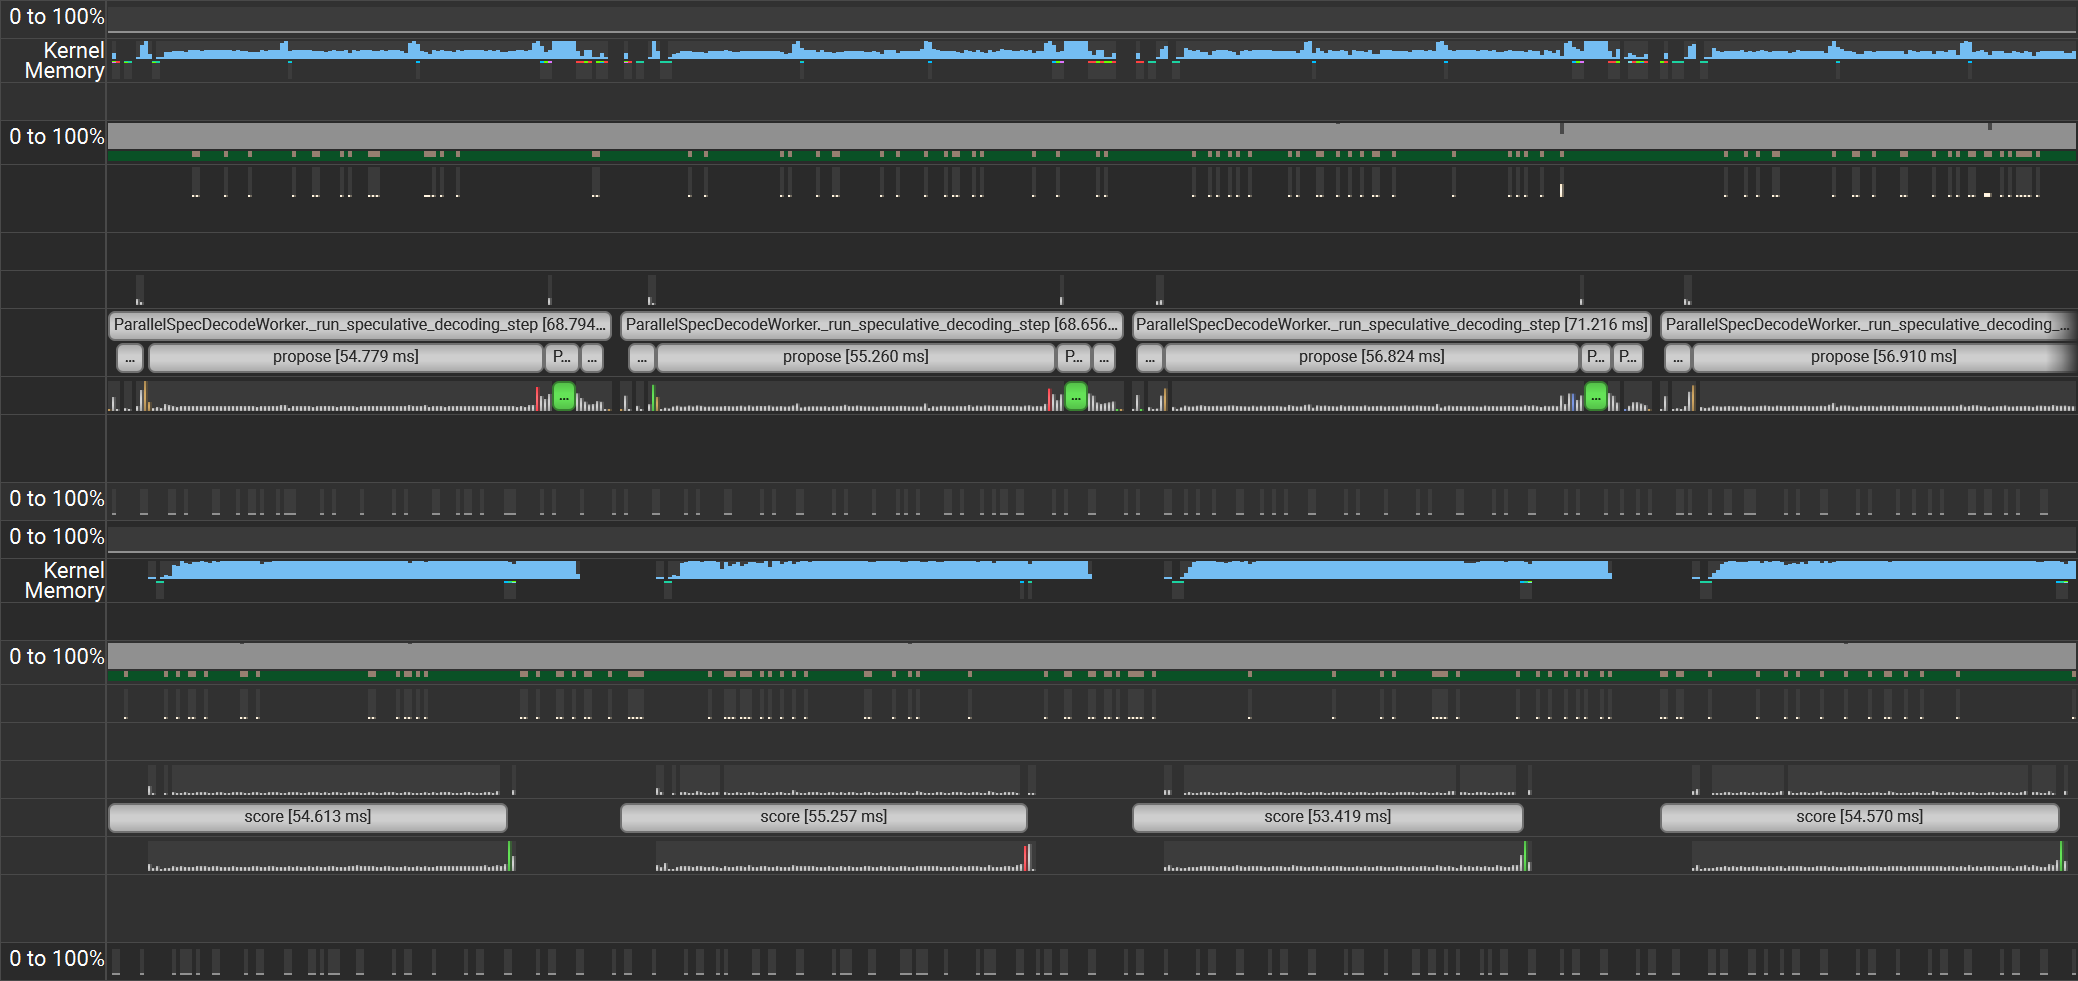
\includegraphics[width=\linewidth, height=0.25\textheight, keepaspectratio]{figures/Qwen3-32B_1.7B_k3.png}
        \par\vspace{5pt}
        \textbf{(c)} Sample segment of Nsight profiling results with model setting 2, Spec-Bench dataset, and $k=3$. Median drafting and verification times are 49.53 ms and 49.30 ms, respectively, suggesting \alg{} almost perfectly overlaps drafting with verification under this configuration.
    \end{minipage}
    \hfill
    \begin{minipage}[t]{0.48\textwidth}
        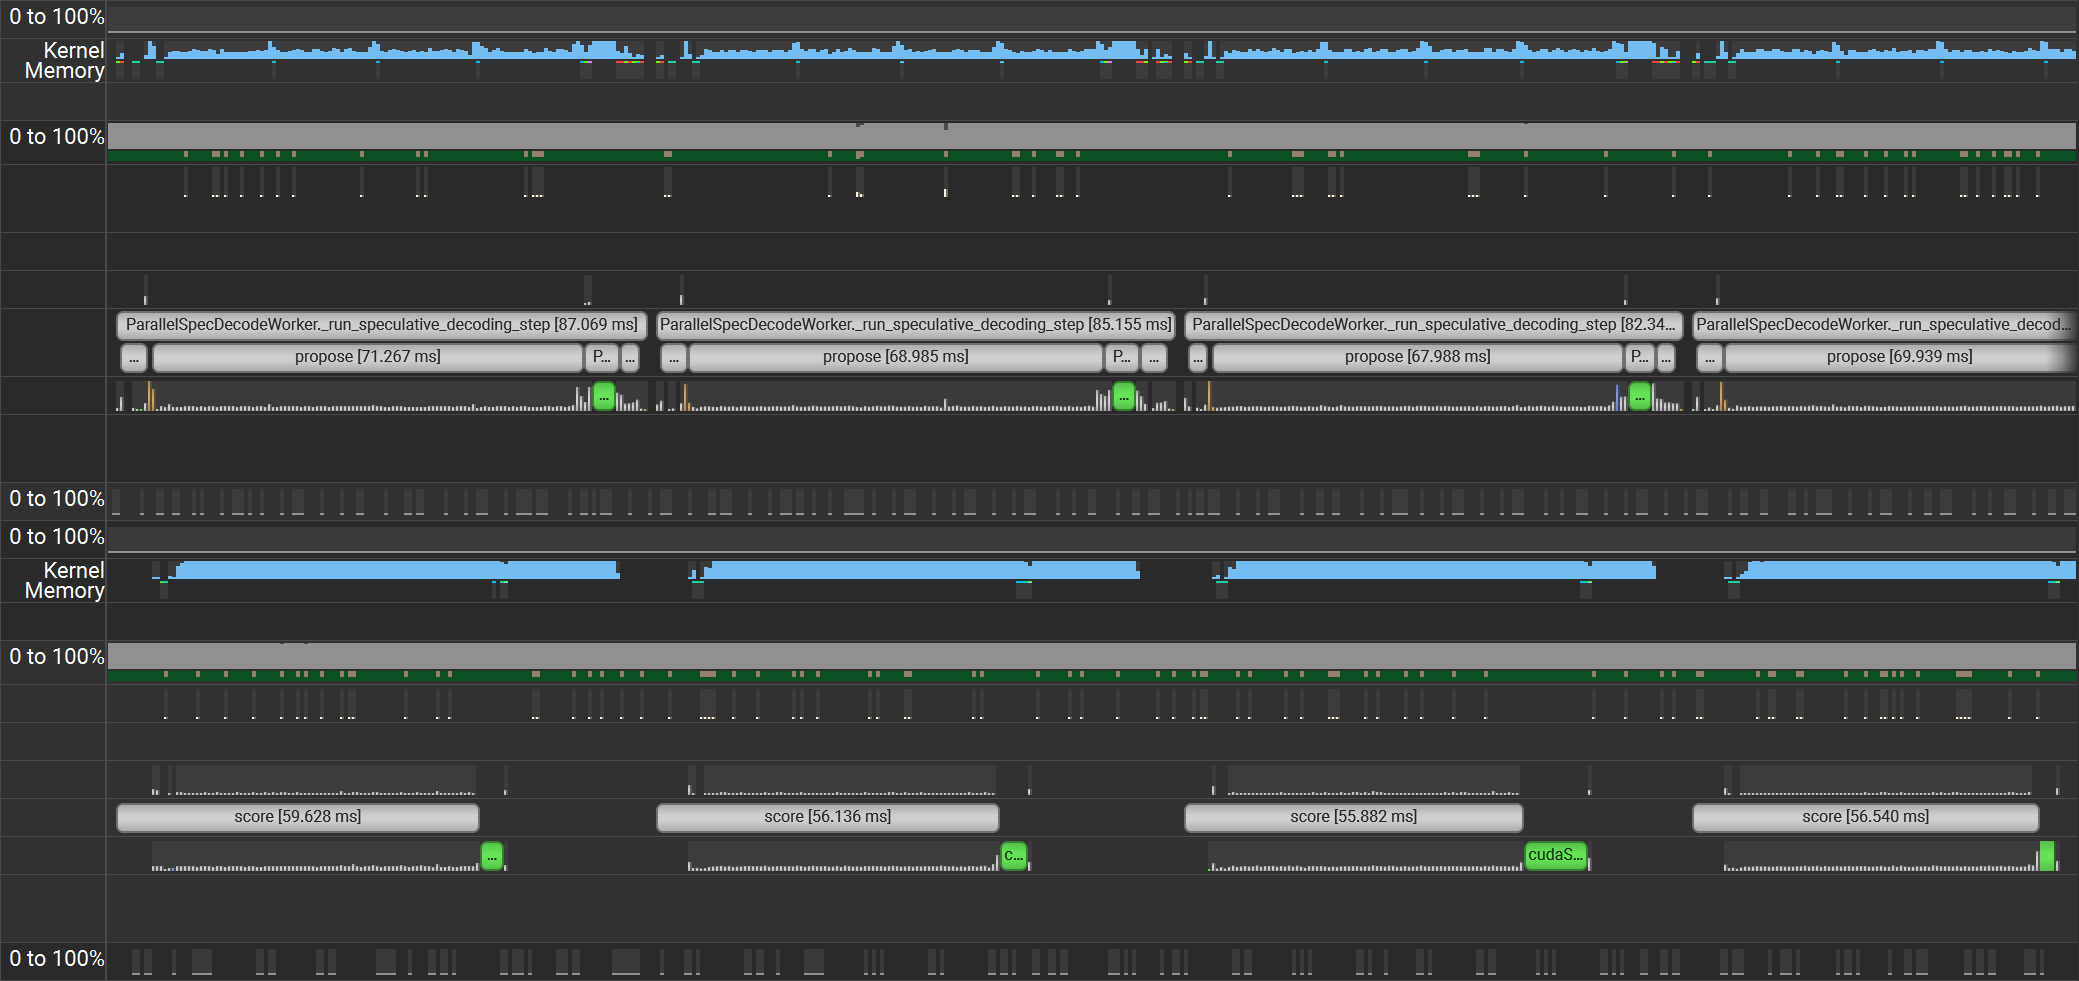
\includegraphics[width=\linewidth, height=0.25\textheight, keepaspectratio]{figures/Qwen3-32B_1.7B_k4.png}
        \par\vspace{5pt}
        \textbf{(d)} Sample segment of Nsight profiling results with model setting 2, Spec-Bench dataset, and $k=4$. Median drafting and verification times are 65.75 ms and 50.70 ms, respectively, suggesting drafting time exceeds verification time by 29.68\%, and the performance of \alg{} may degrade under this configuration.
    \end{minipage}

    \vspace{0.5cm} 
    \begin{minipage}[t]{0.48\textwidth}
        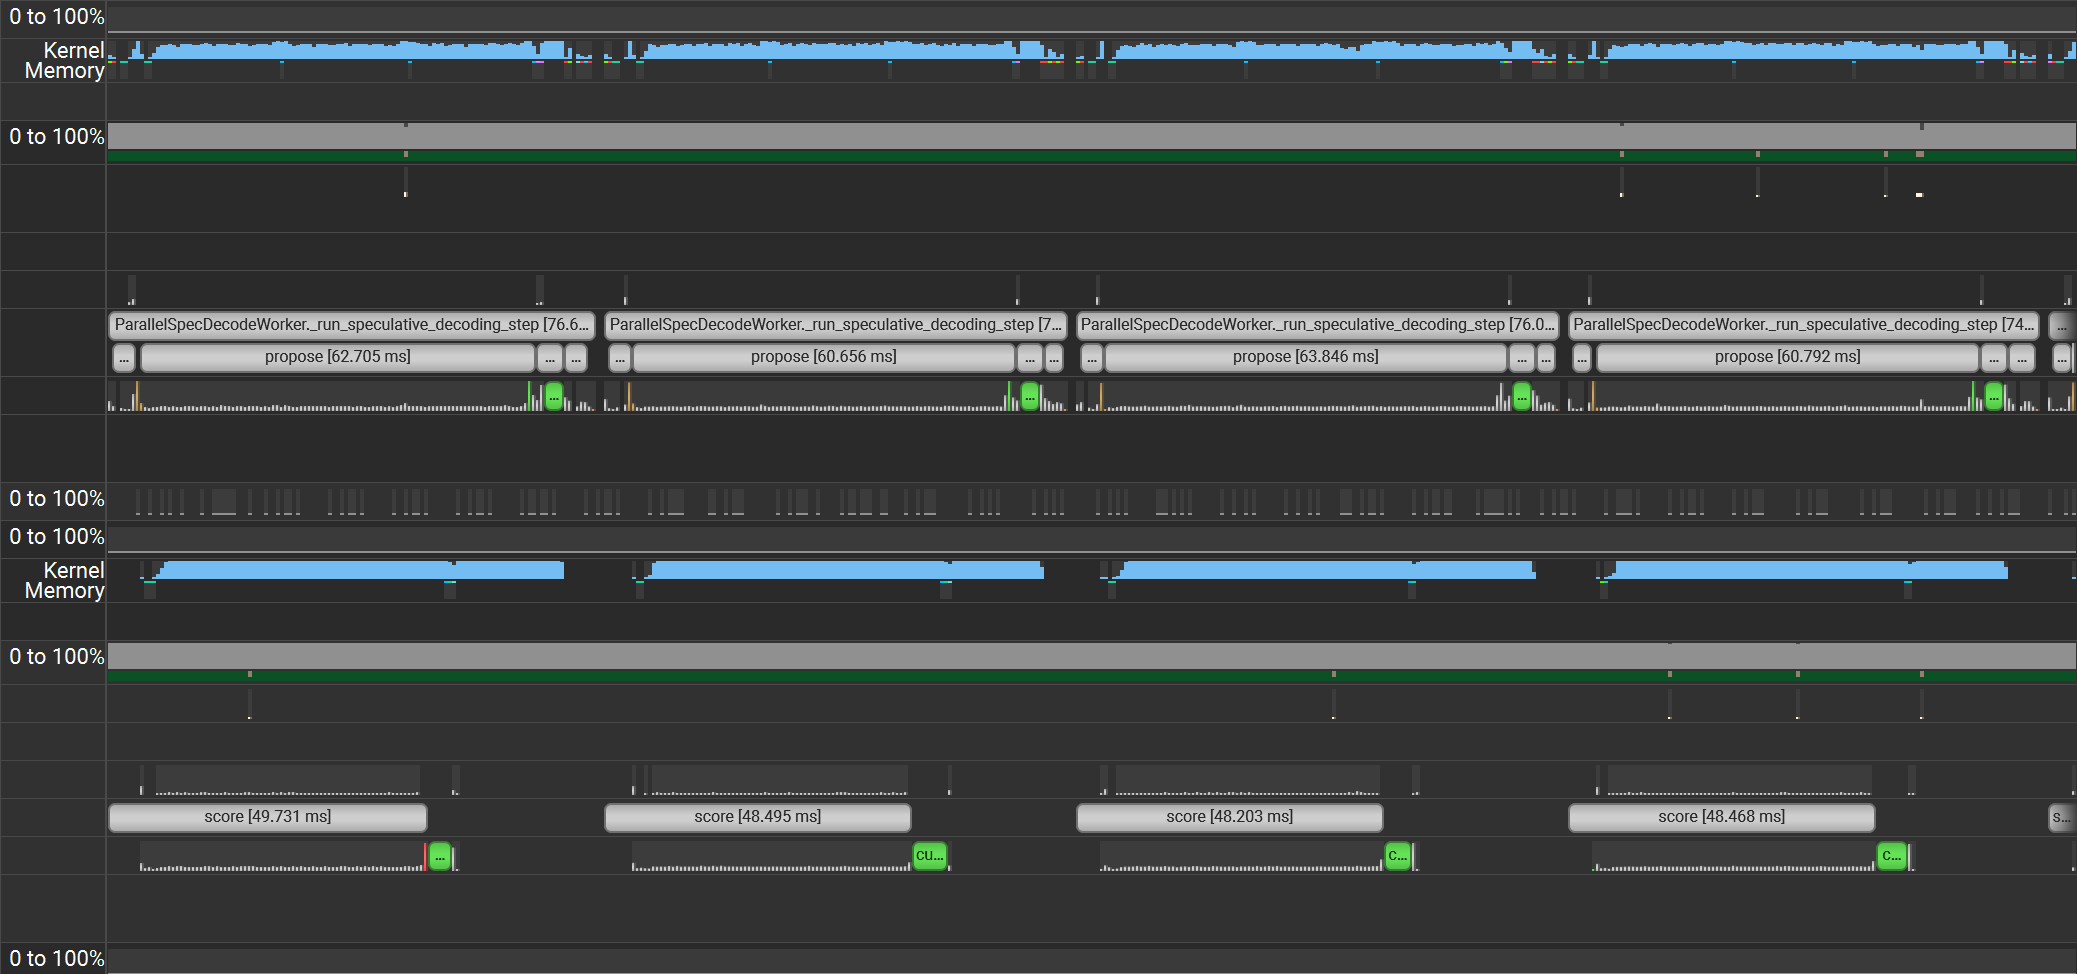
\includegraphics[width=\linewidth, height=0.25\textheight, keepaspectratio]{figures/Qwen3-32B_4B_k3.png}
        \par\vspace{5pt}
        \textbf{(e)} Sample segment of Nsight profiling results with model setting 3, Spec-Bench dataset, and $k=3$. Median drafting and verification times are 61.83 ms and 47.62 ms, respectively, suggesting drafting time exceeds verification time by 29.86\%, and the performance of \alg{} may degrade under this configuration.
    \end{minipage}
    \hfill
    \begin{minipage}[t]{0.48\textwidth}
        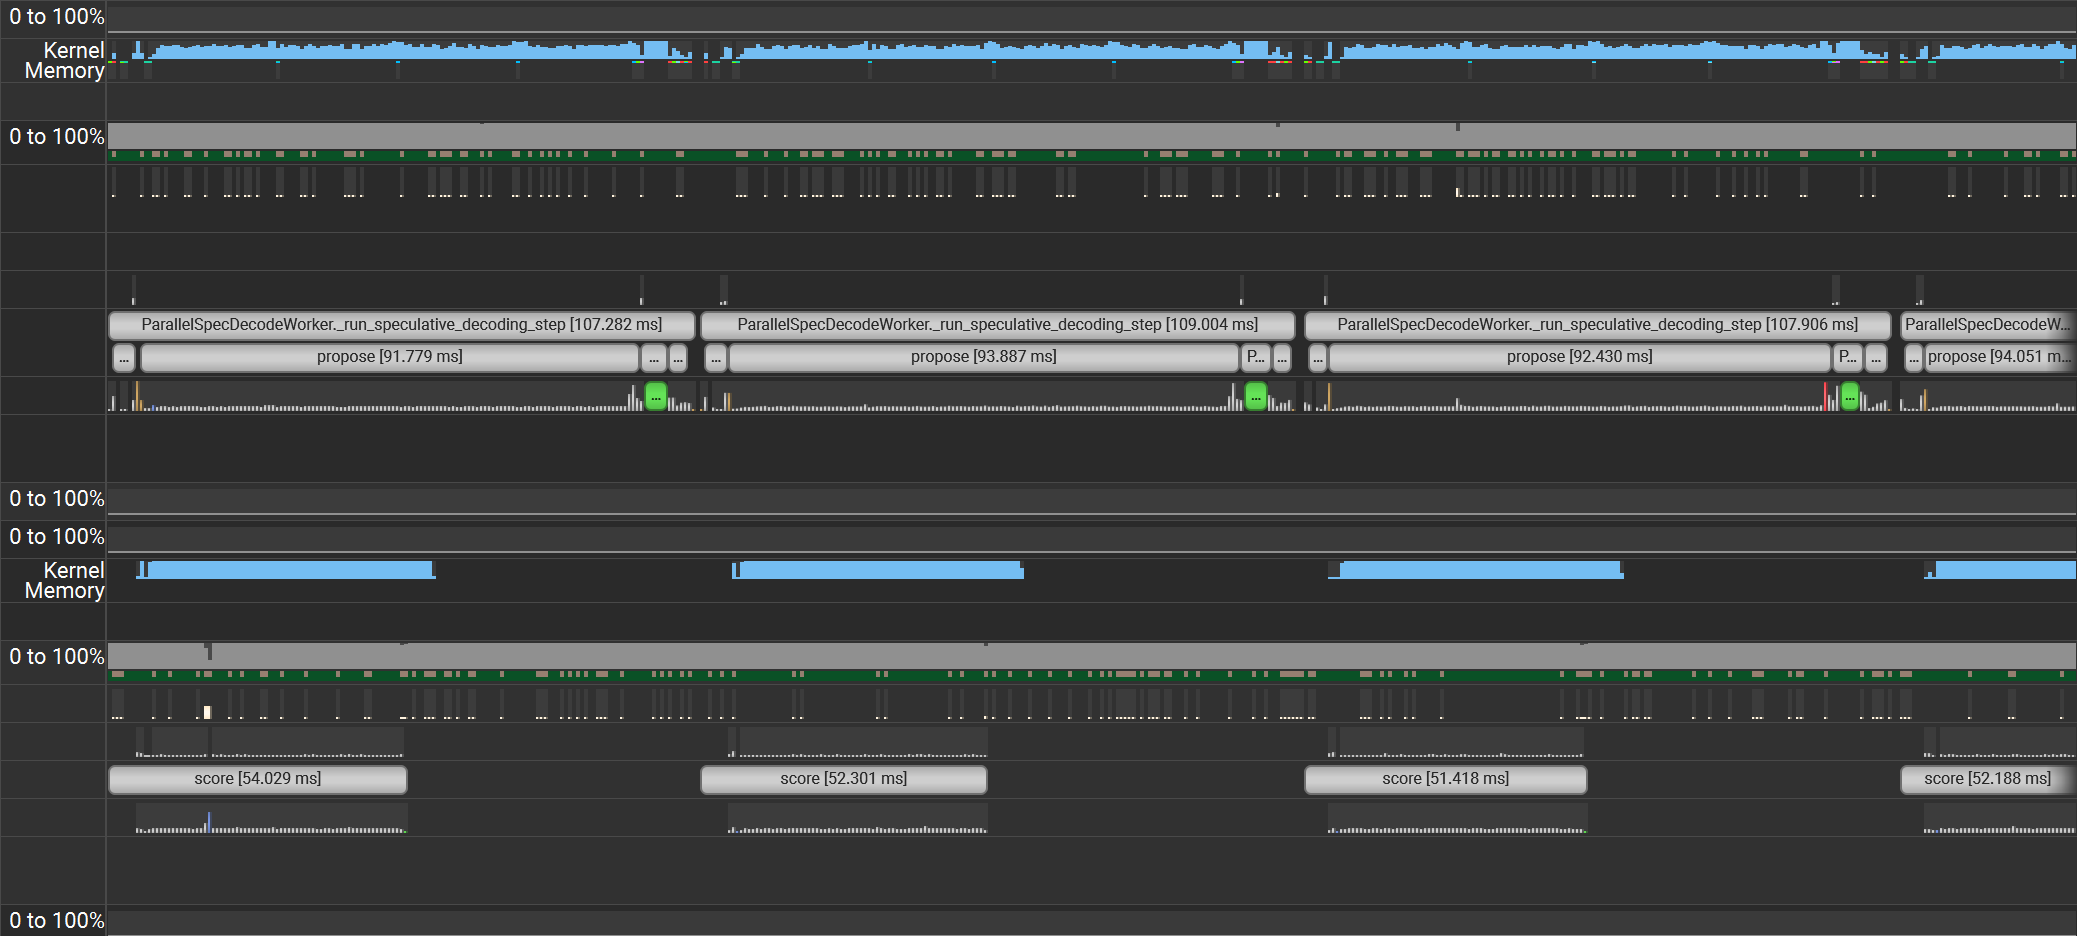
\includegraphics[width=\linewidth, height=0.25\textheight, keepaspectratio]{figures/Qwen3-32B_4B_k4.png}
        \par\vspace{5pt}
        \textbf{(f)} Sample segment of Nsight profiling results with model setting 3, Spec-Bench dataset, and $k=4$. Median drafting and verification times are 81.00 ms and 48.93 ms, respectively, suggesting drafting time exceeds verification time by 65.52\%, and the performance of \alg{} is highly likely to degrade under this configuration.
    \end{minipage}
    \caption{Comparison of Nsight profiling across 6 different configurations.}
    \label{fig:nsight_all}
    \vspace{-4mm}
\end{figure}





\subsection{Nsight Profiling Results}
\label{app:nsight}
Nsight profiling on Settings~1--3 using the Spec-Bench dataset shows that Qwen3-1.7B and Qwen3-0.6B exhibit similar drafting times, whereas Qwen3-4B has the longest drafting time among the three draft models. As illustrated in \cref{fig:nsight_all}, Qwen3-4B spends significantly more time on drafting than the verification time, limiting its ability to benefit from PSD. In contrast, Qwen3-1.7B, while slightly slower than Qwen3-0.6B, has greater model capacity and is thus more effective at generating draft tokens that pass verification. This observation supports the conclusion in \cref{app:exp-draft-model} that Qwen3-1.7B achieves the optimal balance between drafting speed and draft quality.